\RequirePackage{latexml}
\iflatexml
\documentclass[12pt,a4paper,twoside]{book}
\else
\documentclass[paper=a4,
					fontsize=12pt,
				headsepline,
				cleardoublepage=plain,
				numbers=noenddot,
				bibliography=totoc,
				enabledeprecatedfontcommands]{scrbook}
\fi

% from l2tabu.tex
\usepackage[OT2,OT1]{fontenc}                    % needs package cyrillic and lh
\usepackage[russian,ngerman,english]{babel}		% English language settings
\usepackage[utf8]{inputenc}     						% use utf-8, so we have no problems with "umlauts"

%\usepackage[T1]{fontenc}								% T1-fonts

%\usepackage{mathptmx}									% Times/Mathe \rmdefault
%\usepackage[scaled=.90]{helvet}						% scaled Helvetica \sfdefault
\usepackage{helvet} 										% Helvetica \sfdefault
\usepackage{courier}       							% Courier \ttdefault

%\setkomafont{sectioning}{\rmfamily\bfseries}
%\setkomafont{pagehead}{\scshape}

% Additional packages 
\usepackage{natbib}	            % better bibliography and more
                                 % flexible \cite-command
\usepackage[intlimits]{amsmath}	% more mathematical symbols
\usepackage{amsthm,amsfonts}		% more mathematical environments and fonts
\usepackage{graphicx}				% for including of images
\usepackage{color}     				% necessary to include .pstex_t files from xfig!!!
\usepackage[font=small, format=plain, labelfont=bf]{caption}		% more flexible captions
\usepackage[tight]{subfigure}		% support for subfigures (should be replaced
											% by the newer "subfig" package
\usepackage{units}					% support for physical units
%\usepackage{isotope}				% support for writing isotopes
%\usepackage{esint}   				% must be loaded after amsmath

% not includes in standard latex environment
\usepackage{aas_macros}				% support for abbreviations from AAS-Journal 
%\usepackage{ziffer}					% only possible with MikTex

% the hyperref package for hyperlinks should be included as last package
\usepackage[pdftex,
				breaklinks=true,  	% some links do not work, if this option is set
				colorlinks=true,  	% before printout, set to false!!!
				linkcolor=blue,
				citecolor=blue,
				urlcolor=blue,
				pagebackref=true]{hyperref}

% use normal fontstyle for urls; if not set, a tt-font is used
\urlstyle{same}

%\usepackage{ae,aecompl}

\pagestyle{headings}

% distance of line from head:
\headsep4mm

% recompute type area
\typearea[10mm]{current}		

% no indentation at the beginning of a new paragraph
%\setlength{\parindent}{0pt}

% change caption with package caption2
%\renewcommand{\figurename}{Abb.}
\addto\captionsngerman % see http://www.faqs.org/faqs/de-tex-faq/part8/
{
    \renewcommand{\figurename}{Fig.}%
    \renewcommand{\tablename}{Tab.}%
}
%\renewcommand{\captionlabelfont}{\bf}
%\renewcommand{\captionlabeldelim}{.}

% new commands for math mode

% vector and absolute value
\newcommand{\abs}[1]{\left\lvert#1\right\rvert}
\renewcommand{\vec}[1]{\boldsymbol{#1}}

% vector operators
\DeclareMathOperator{\grad}{grad}
\DeclareMathOperator{\Div}{div}    %\div is used by amsmath
\DeclareMathOperator{\rot}{rot}

% brackets
\newcommand{\lra}[1]{{ \left( #1 \right) }}
\newcommand{\lrb}[1]{{ \left[ #1 \right] }}
\newcommand{\lrc}[1]{{ \left\{ #1 \right\} }}

% filtered quantities
%\newcommand{\fil}[1]{{<} #1 {>}}
\newcommand{\fil}[1]{\langle #1 \rangle}
\newcommand{\ffil}[1]{{\ll} #1 {\gg}}
\newcommand{\cfil}[1]{{\prec}#1{\succ}}
\newcommand{\chat}[1]{\accentset{\curlywedge}{#1}}
\newcommand{\ol}[1]{\overline{#1}}

% fractions
\newcommand{\td}[1]{\frac{d}{d #1}}
\newcommand{\ttd}[2]{\frac{d #2}{d #1}}
\newcommand{\pd}[1]{\frac{\partial}{\partial #1}}
\newcommand{\ppd}[2]{\frac{\partial #2}{\partial #1}}
\newcommand{\pdd}[1]{\frac{\partial^2}{\partial #1^2}}
\newcommand{\fa}{\frac{1}{a}}
\newcommand{\fh}{\frac{\dot{a}}{a}}
\newcommand{\ft}{\frac{1}{\sqrt{2\pi}}}
\newcommand{\fft}{\frac{1}{2\pi}}
\newcommand{\ffft}{\frac{1}{(2\pi)^{3/2}}}

% integrals
\newcommand{\iinf}{\int_{-\infty}^{\infty}}
\newcommand{\iiinf}{\iint_{-\infty}^{\infty}}
\newcommand{\iiiinf}{\iiint^{\infty}_{-\infty}}


%\titlehead{Institut für Theoretische Physik und Astrophysik \\
%Julius-Maximilians-Universität Würzburg}
\title{\Huge{Adaptively Refined Large-Eddy Simulations of Galaxy Clusters}}
\author{
\\
\\
\\
Dissertation zur Erlangung des \\ 
naturwissenschaftlichen Doktorgrades \\ 
der Bayerischen Julius-Maximilians-Universität Würzburg\\ 
\\
\\
vorgelegt von \\ 
\textbf{Andreas Maier} \\ 
aus Coburg\\
\\
\\
\\
\\
\\
\\
\\
}
\date{}
\publishers{Würzburg 2008}
\uppertitleback{
\vspace{5cm}
Eingereicht am\\
bei der Fakultät für Physik und Astronomie
\\
\\
\\
1. Gutachter: Prof. Dr. Jens Niemeyer\\
2. Gutachter:\\
der Dissertation\\
\\
\\
\\
1. Prüfer: Prof. Dr. Jens Niemeyer\\
2. Prüfer:\\
3. Prüfer:\\
im Promotionskolloquium\\
\\
\\
\\
Tag des Promotionskolloquiums:\\
\\
\\
Doktorurkunde ausgehändigt am \ \underline{\hspace{3cm}}
}
 
%\dedication{\dictum[Homer Simpson]{Don’t worry head. The computer will do
% all the thinking from now on.}}
% \dedication{\dictum{Journalist: Any disappointments?\\
% Feynman: Certainly. I’ve spent years trying to solve some difficult problems
% without success. The theory of turbulence is one. In fact, it is still
% unsolved.}}
\dedication{\foreignlanguage{russian}{Posvyashchayu Olp1ge}}


\begin{document}
\maketitle
\tableofcontents

\chapter{Introduction}
\section{Historical overview}
Clusters of galaxies are the largest and most recent gravitationally-relaxed
structures in the universe. They typically contain hundreds to thousands of
galaxies with a total mass of about $10^{14} - 10^{15}$ solar masses
($\unit{M_{\odot}}$), spread over a region whose size is roughly 10 million
light-years ($\unit{Mly}$). Galaxy clusters themselves form even greater
structures called superclusters, which are gravitationally-attracted, but not
relaxed, collections of ten to one hundred clusters and groups of galaxies. The
Milky
Way itself belongs to the ``Local Group'' , which is an aggregation of
about 40 galaxies, with the Andromeda Galaxy and the Milky Way as the largest
members of
the group. The Local Group belongs to the ``Virgo Supercluster'', with the
Virgo cluster at the center. The Virgo cluster is the nearest cluster of
galaxies to our own galaxy at a distance of 60 Mly; another famous cluster of
galaxies is the Coma cluster, which is called a very regular cluster,
because it is nearly spherically symmetric (see figure \ref{fig:comavis}).
\begin{figure}[tp]
\centering
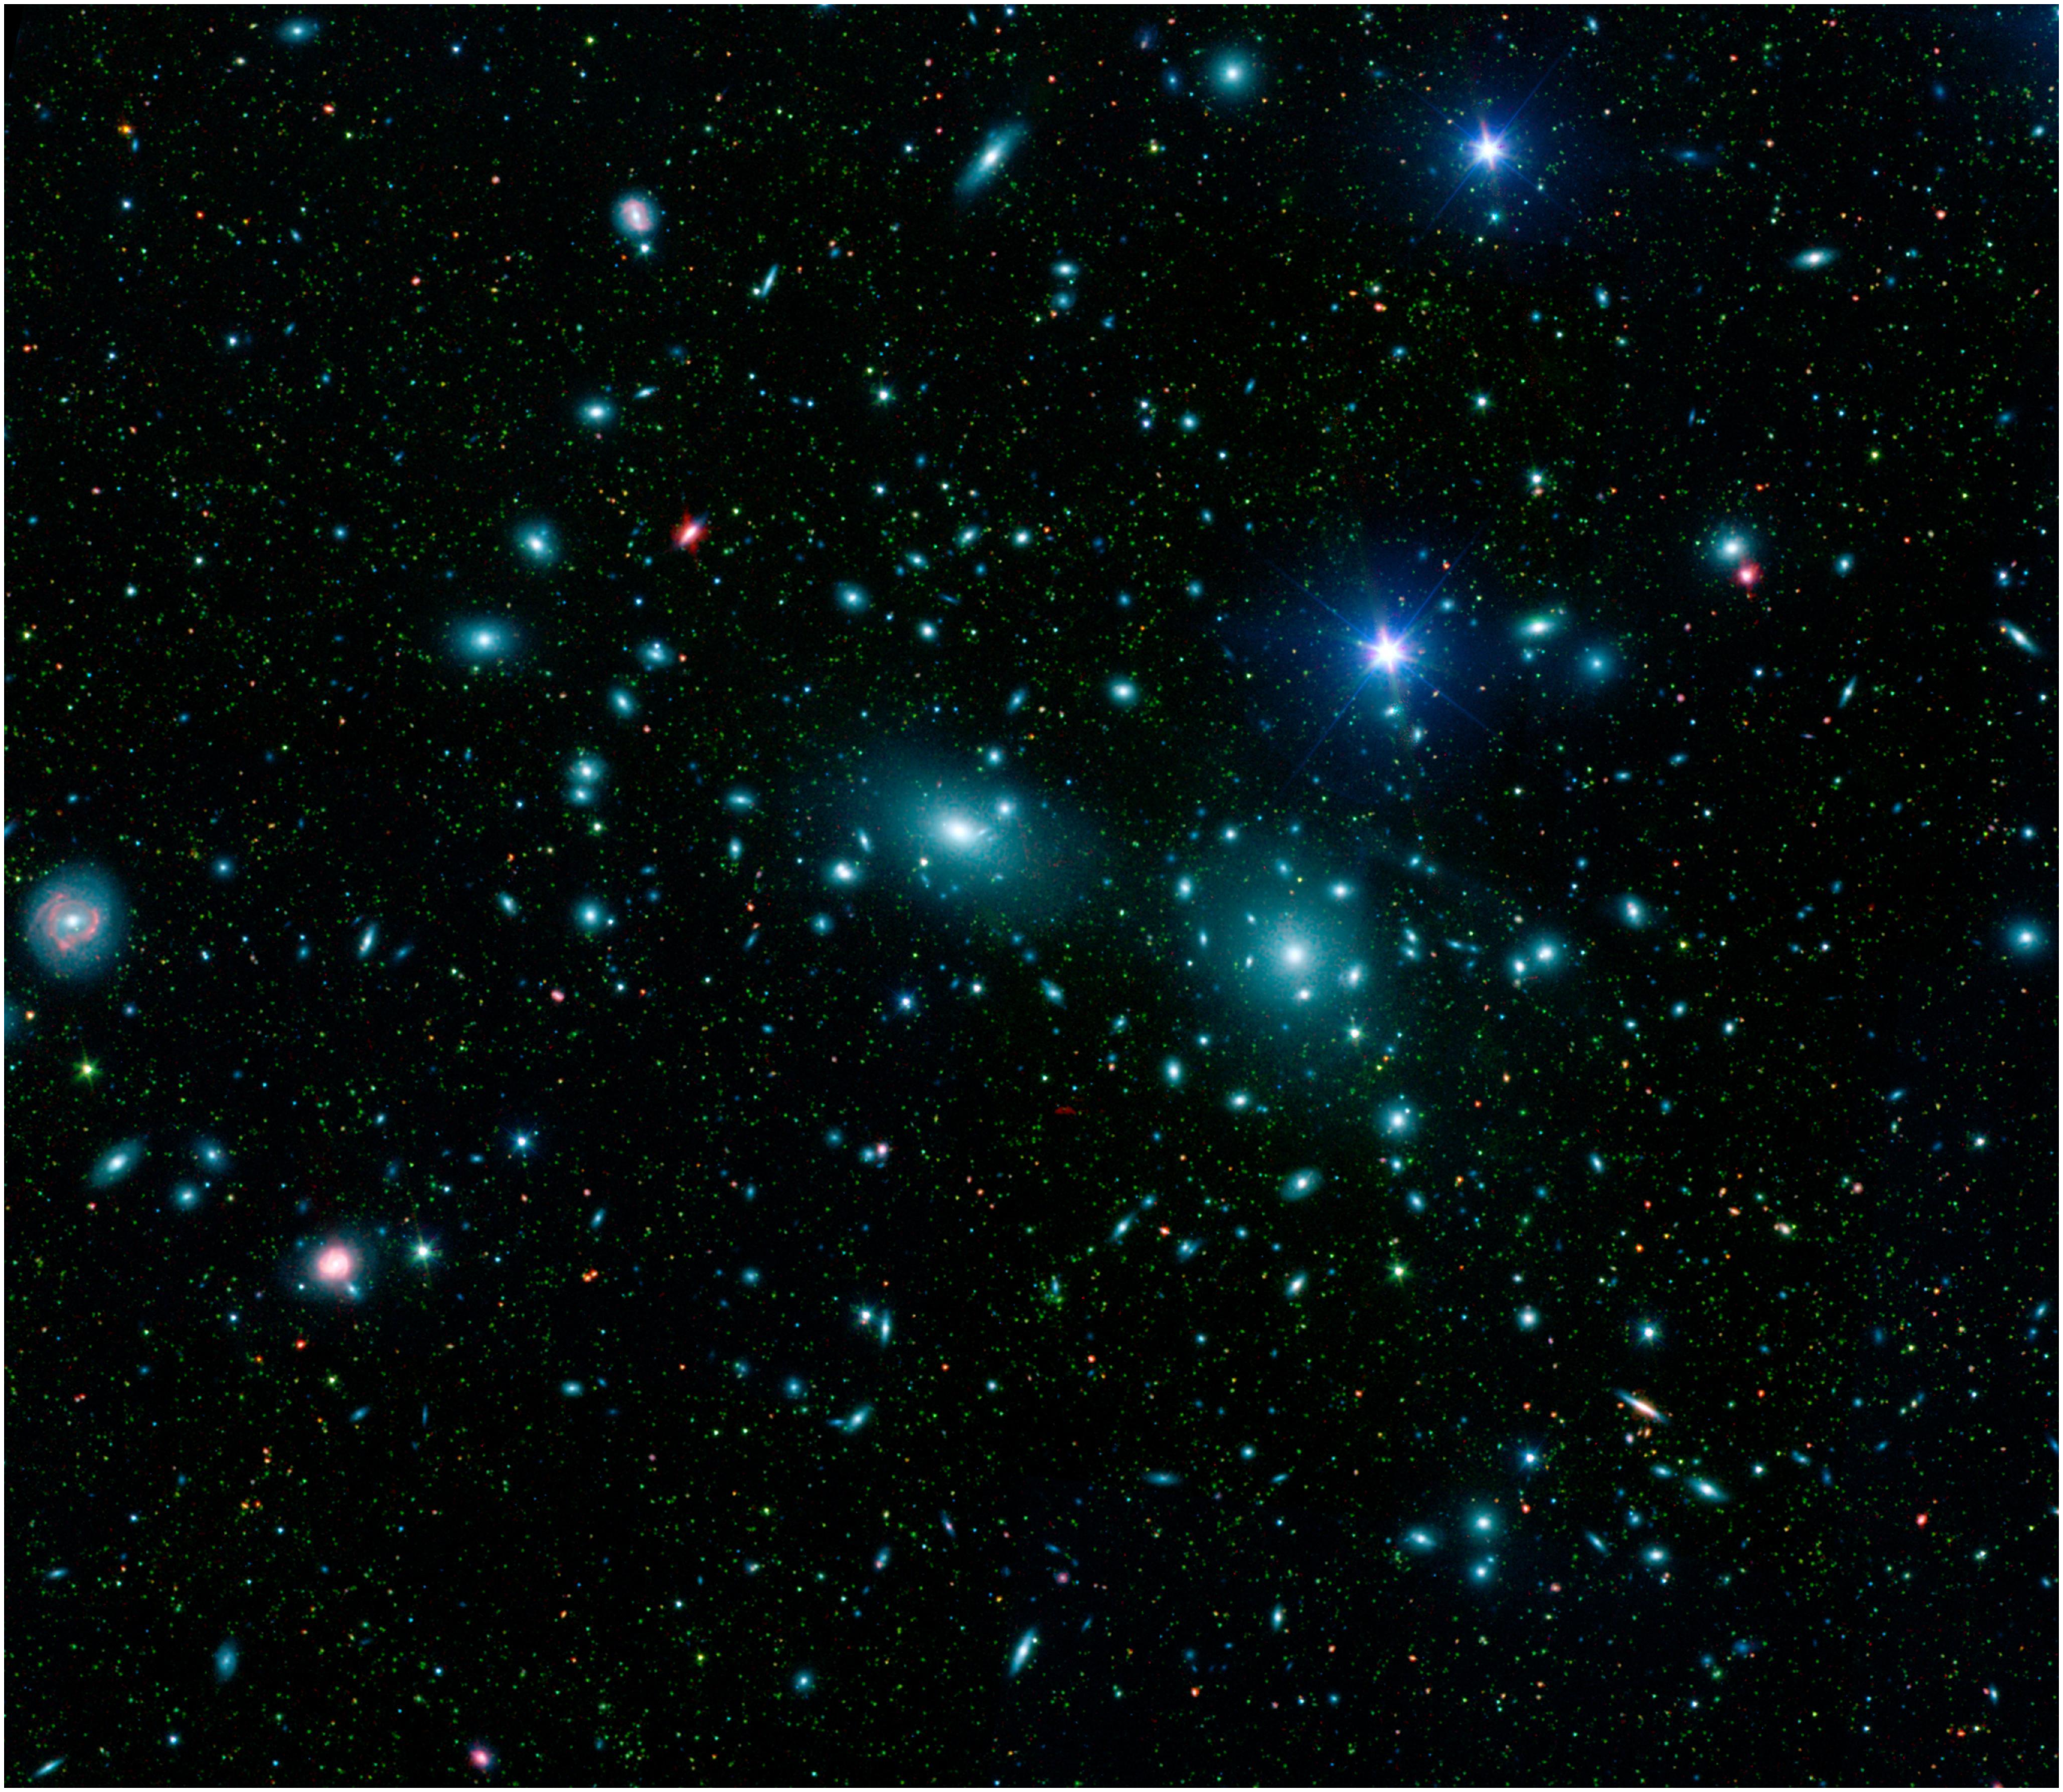
\includegraphics[width=0.7\linewidth]{chapter1/Comacluster_nasajpl.eps}
\caption{A Sloan Digital Sky Survey/Spitzer Space Telescope image of the Coma
Cluster in ultraviolet and visible light. From \citet{Jenkins2007}.}
\label{fig:comavis}
\end{figure}

The tendency of galaxies to form clusters in the sky has long been noticed (for
example \citet{Messier1784} had identified already 16 galaxies, which - as we
now know - belong to the Virgo cluster, and he noted that they form a
group), but
the first to study them in detail was \citet{Wolf1906}. A great step forward in
the systematic study of the properties of clusters was the work of
\citet{Abell1958}, who compiled the first extensive, statistically complete
catalog of so-called rich clusters of galaxies\footnote{The richness of a galaxy
is a measure that is basically proportional to the number of bright galaxies in
a cluster. It was first strictly defined by Abell for his catalog.}. This
catalog and its successors (e.g. \citet{Abell1989}) are the foundation for much
of our modern understanding of clusters.   

The cited catalogs of clusters are based on optical identification techniques.
However in the early 1970s extended x-ray emission from clusters of galaxies
was observed by \citet{Gursky1971, Kellogg1972}, which had been already
correctly attributed to thermal
bremsstrahlung several years earlier by \citet{Felten1966}. This interpretation
requires
the space between galaxies in clusters to be filled with a very hot 
($\approx \unit[10^8]{K}$) low density ($\approx \unit[10^3]{atoms/m^3}$) gas.
Remarkably, the total mass in this intracluster medium (ICM) is comparable to
the total mass of all galaxies in the cluster. Nevertheless this discovery did
not solve the so called missing mass problem in clusters, which was first
formulated by \citet{Zwicky1933,Zwicky1937}. \citet{Zwicky1933} was the first
to measure the velocity dispersion of galaxies in the Coma cluster, finding
$\sigma_{galaxy}=\unit[700]{km\ s^{-1}}$, and he correctly concluded from this
fact and his estimate of the Coma's cluster overall radius, that the cluster
mass, which he computed using the virial theorem, must be far greater than the
observed luminous mass - the first evidence for dark matter in the universe. In
his remarkable paper of 1937, Zwicky also proposed gravitational lensing as an
alternative technique for measuring the masses of background galaxies. This
technique finally became practicable after six more decades \citep{Tyson1990},
and is now a standard technique for measuring cluster mass
\citep{Bartelmann2003}.

Measuring the masses of clusters is not only important for the search of dark
matter. Some of the most powerful constraints on current cosmological models
come from observations of how the cluster mass function $n(M)$, which gives the
number density of clusters with a mass greater than $M$ in comoving volume
element, evolves with time \citep{Voit2005}. The reason why the evolution of the
cluster mass function is so highly sensitive to cosmology is simply because the
matter density of the universe controls the rate at which structure grows. 
The cluster mass function can be measured using optical surveys.
However it is easier to use X-ray surveys, because in the X-ray band, instead of
a collection of galaxies, each cluster appears only as a single source (see
figure \ref{fig:comaxray}), 
\begin{figure}[tp]
\centering
\includegraphics[width=0.62\linewidth]{chapter1/0150_xray.eps}
\caption{Chandra X-ray image of the central region of the Coma Cluster. From
\citet{Vikhlinin2002}.}
\label{fig:comaxray}
\end{figure}
which makes it observationally easier to define consistently
cluster properties like the radius. Independently from Supernova IA and cosmic
microwave background (CMB) measurements, these and other cluster-related
surveys can now restrict several important parameters of the cosmological
concordance model (see figure \ref{fig:omegas}). 
\begin{figure}[tp]
\centering
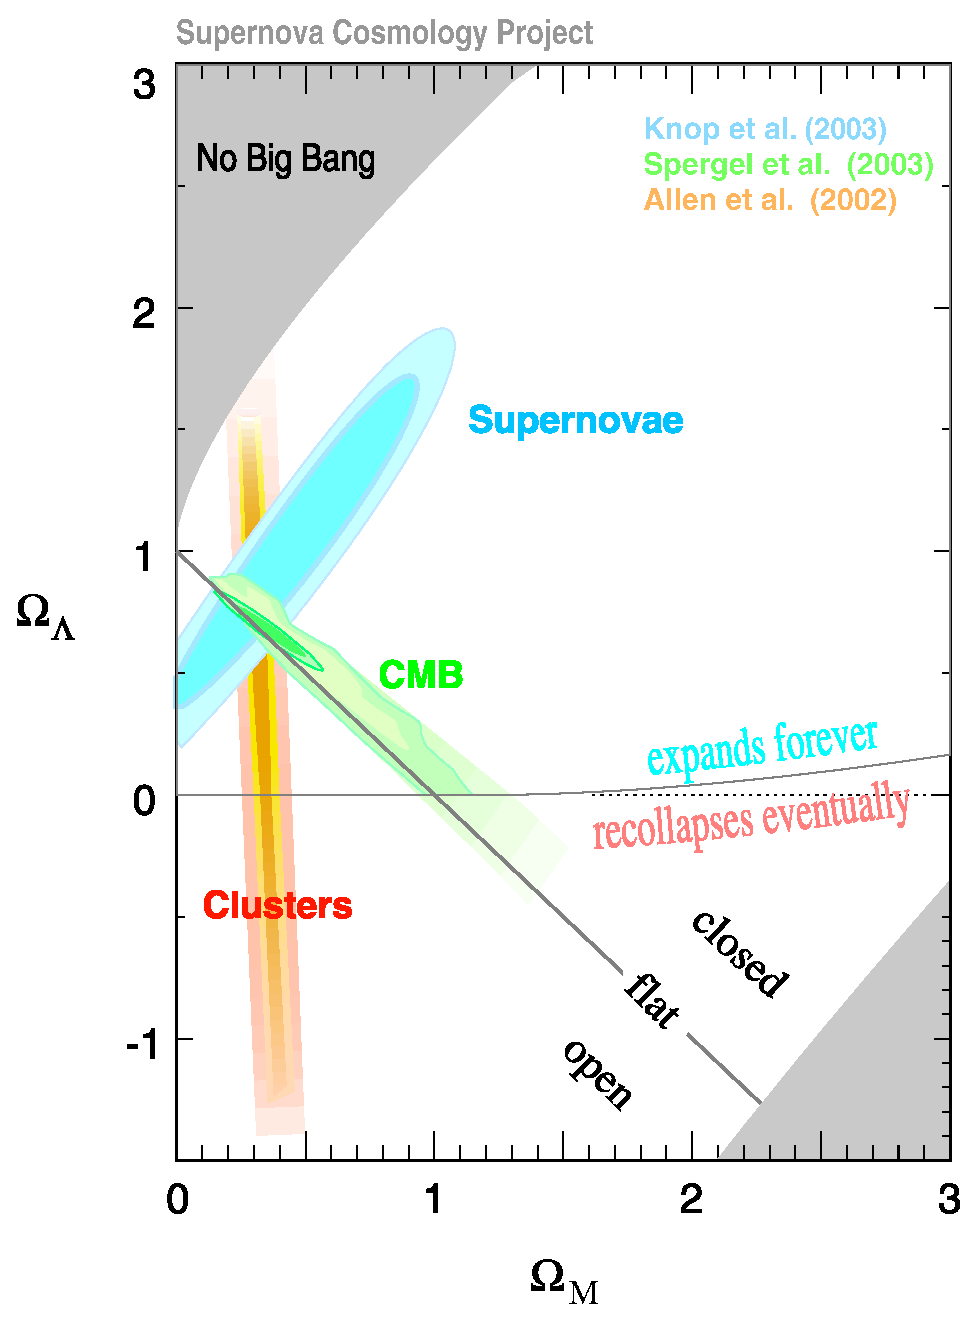
\includegraphics[width=0.45\linewidth]{chapter1/SCP2003SNeCMBClust.eps}
\caption{Plot of 68\% and 90\% confidence regions for $\Omega_M$
and $\Omega_{\Lambda}$ for Supernova IA, CMB and cluster data. From
\citet{Knop2003}.
}
\label{fig:omegas}
\end{figure}

Most of these cluster surveys make use of several
relations like the mass-temper\-ature or luminosity-temperature relation, which
are only based on observational findings. If gravity alone would determine
the thermodynamical properties of the clusters, we would expect clusters to be
self-similar, meaning clusters of different size would be scaled versions of
each other, leading to a specific simple form of these relations
\citep{Kaiser1986}.
However astronomers have known for more than a decade that the intracluster
medium cannot be self-similar, because the luminosity-temperature
relation of clusters does not agree with self-similar scaling \citep{Voit2005}.
So only by breaking the self-similar scaling of clusters can the
observed relations be explained. But it is theoretically
still uncertain, which mechanism(s) is (are) responsible for that similarity
breaking. Many mechanisms have been proposed including preheating, radiative
cooling, feedback from supernovae, feedback from active galactic nuclei
\citep{Voit2005}, shocks, magnetic fields, cosmic rays and turbulence 
\citep{Dolag2008}. It therefore remains a challenge for the theory of cluster
physics to find the responsible mechanisms and explain the relations mentioned
above.

\section{Aim of this work}
One of the proposed mechanisms that break gravitationally self-similar scaling
properties of clusters is turbulence. Turbulence is also believed to
play an important role in explaining the magnetic field strengths of galaxy
clusters and the higher than expected temperature of cluster cores (the 
``cooling flow problem''). However numerical simulations of the
influence of turbulence in an astrophysical context in general and especially
for clusters have been restricted to measuring passively statistical
quantities
like velocity dispersion from simulation data (e.g. \citet{Dolag2005}). 
The active role of small scale velocity fluctuations on the large scale flow
could not be treated at all. There are two main reasons for this:
\begin{enumerate}
\item Basically turbulence is a physical phenomenon that is far from
being understood. The sole currently  existing theory is only
applicable to isotropic, incompressible turbulence. No accepted theoretical
framework for
describing turbulent flows in astrophysical environment including compressible,
selfgravitating, high Mach number flows exists. 
\item Models describing the effective influence of turbulence in fluid dynamic
simulations are restricted to a specific length scale. They are not suitable to
treat the vast range of different length scales (from cosmological scales
$\approx \unit[10^{24}]{m}$
down to the thickness of a shock front ($\approx \unit[10^{11}]{m}$,
\citet{Medvedev2006}) we need to address
when simulating astrophysical environments.
\end{enumerate}
Therefore it is aim of this work to develop, implement, and apply a new
numerical scheme for modeling turbulent, multiphase astrophysical flows such as
galaxy cluster cores and star forming regions. The method combines the
capabilities of adaptive mesh refinement (AMR) and large-eddy simulations (LES)
to capture localized features and to represent unresolved turbulence,
respectively; it will be referred to as Fluid mEchanics with
Adaptively Refined Large-Eddy SimulationS or FEARLESS. 

To start explaining the idea behind this ansatz, we first give a brief overview
of the theory of turbulence in chapter \ref{turbulence}. In chapter \ref{filter}
we introduce a filter formalism, which is necessary for modeling compressible
turbulence according to the ideas of LES. In chapter \ref{FE} we use this
formalism to derive the filtered equations of fluid dynamics, which are the
basis for the introduction of our turbulence or subgrid scale (SGS) model
(adapted from work by \citet{Schmidt2006}) in chapter \ref{LES}.
In this chapter we also analyse in some detail the
influence of the turbulence model on the equation of fluid dynamics. In chapter
\ref{amrles} we explain the specific problem of combining LES and AMR in
some detail and propose a new method to circumvent this problem. In chapter
\ref{numtest} we comment on several modifications and numerical issues that
had to be taken into account when implementing our method into the cosmological
fluid code Enzo. We also present the results of several driven turbulence test
simulations, showing the consistency of our treatment of turbulence. Chapter
\ref{clustertheo} summarizes some important facts about cluster physics and we
also give a brief introduction to turbulence in cluster simulations.
In chapter \ref{clustersim} we describe several issues with our turbulence model
when treating turbulence in cluster simulations on cosmological scales. We
explain our setup and then describe the main results of a first study of
turbulence in galaxy cluster simulations using our FEARLESS approach. Finally in
chapter \ref{summ} we
summarize our findings and draw conclusions about the influence of turbulence
in the context of cluster simulations. 


\chapter{Turbulence}\label{turbulence}
The equations for a general compressible, viscous, selfgravitating fluid 
with density $\rho(r_i,t)$, momentum density $\rho v_i(r_i,t)$ and total
energy density $\rho e(r_i,t)$ are\footnote{see eg. \citet{Landau1991}.}
\begin{align}
\pd{t}\rho + \pd{r_j}(v_j \rho) &= 0, \label{eq:mass}\\
\pd{t}(\rho v_i) + \pd{r_j}(v_j \rho v_i) &= -\pd{r_i}p + \pd{r_j}\sigma'_{ij}
+\rho g_i, 
\label{eq:mom} \\
\pd{t}(\rho e) + \pd{r_j}(v_j \rho e) &= -\pd{r_j}(v_j p) + \pd{r_j}(v_i
\sigma'_{ij}) + v_i \rho g_i,
\label{eq:etot}
\end{align}
with Newtonian gravity (Poisson Equation)
\begin{align}
\pd{r_j}g_j=4\pi G \rho
\end{align}
and an equation of state to compute the pressure $p(r_i,t)$ dependent on
the material of the fluid. For a Newtonian fluid the stress tensor
$\sigma_{ij}$ is of the form\footnote{For a derivation see Appendix
\ref{stress}.}
\begin{align}
\sigma'_{ij} =  
2\eta\lrb{\frac{1}{2}\lra{\ppd{r_j}{v_i}+\ppd{r_i}{v_j}}
-\frac{1}{3}\delta_{ij}\ppd{r_k}{v_k}}
+\zeta \delta_{ij}\ppd{r_k}{v_k},
\end{align}
where the so called dynamic viscosity $\eta$ and the second viscosity $\zeta$
are defined to be constants\footnote{The literature on incompressible flows
often defines the so called kinematic viscosity $\nu=\frac{\eta}{\rho}$. It
should be noted, that this quantity is a constant only for fluids of constant
density and cannot be used in a meaningful way when discussing compressible
flows.} in a Newtonian fluid.

This system of differential equations is complex and highly nonlinear if the
nonlinear advection term $\pd{r_j}(v_j \rho v_i)$ dominates in the momentum
equation \eqref{eq:mom} and in general can be solved only numerically.
The influence of the advection term can be estimated by writing down the 
momentum equation in dimensionless form, which yields\footnote{See Appendix
\ref{dimanal}.}
\begin{align}
\underbrace{\frac{l_0}{v_0 t_0}}_{Sr}\pd{t^*}(\rho^* v_i^*) 
+ \pd{r_j^*}(v_j^* \rho^* v_i^*) &= 
-\underbrace{\frac{p_0}{\rho_0 v_0^2}}_{Ma^{-2}_{iso}}\pd{r_i^*}p^* 
+\underbrace{\frac{\sigma_0}{\rho_0 v_0^2}}_{Re^{-1}}\pd{r_j^*}\sigma_{ij}^*
+\underbrace{\frac{\rho_0 g_0 l_0}{\rho_0 v_0^2}}_{Fr^{-1}} \rho^* g_i^*.
\end{align}
The arising dimensionless numbers\footnote{The Strouhal number
 $Sr$ can be set to one by assuming $v_0=\frac{l_0}{t_0}$.}
($Re$ = Reynolds number, $Ma_{iso}$ =
isothermal Mach number, and $Fr$ = Froude number)
show the ratio of the mean pressure energy density $p_0$, the
mean potential energy density $\rho_0 g_0 l_0$, and the mean energy dissipation
density $\sigma_0$ to the mean kinetic energy density $\rho_0 v_0^2$. 
If all these numbers are much greater than one (which means the mean
kinetic energy is big compared to the other energies), the advection term
dominates and the fluid flow is called turbulent. 

\section{Phenomenology of Turbulence}
As there is no accepted theory of compressible, selfgravitating turbulence we
have to restrict the following discussion to incompressible turbulence. For an
incompressible fluid, it can be shown that the Reynolds number
\begin{align}
Re=\frac{\rho_0 v_0^2}{\sigma_0}=\frac{\rho_0 l_0 v_0}{\eta_0} 
\end{align}
is the only number which characterizes the dynamics of the fluid flow
\citep{Feynman1964}. 

\begin{figure}[tp]
\centering
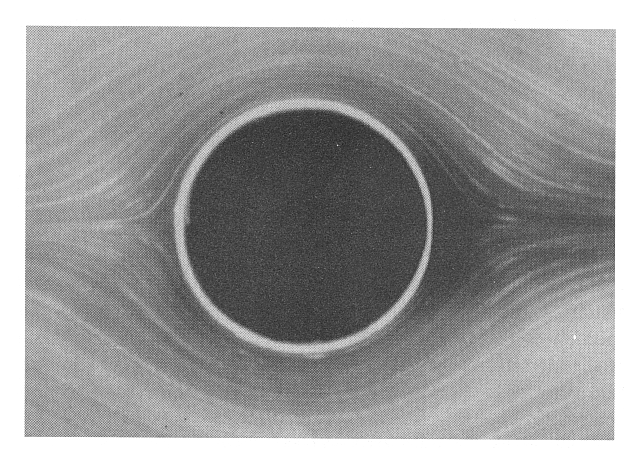
\includegraphics[width=0.7\linewidth]{chapter2/Reynolds0.eps}
\caption{Laminar flow past a cylinder at $Re=0.16$ \citep{Frisch1995}.}
\label{fig:rey0}
\end{figure}

If the Reynolds numbers is small, which is the case for high viscosity and/or
low flow speed, we call the fluid laminar. In this laminar state the streamlines
of the fluid exhibit all the symmetries of the equations and boundary
conditions. This can be seen in figure \ref{fig:rey0}, where the streamlines of
a fluid around a cylinder show up-down and left-right symmetry.\footnote{
Actually the streamlines also show z-invariance (along the axes of the cylinder)
and time-invariance, but they do not show cylindrical symmetry as the direction
of the fluid flow breaks this symmetry.} 

\begin{figure}[tp]
	\centering
	\subfigure[$Re=240$]
	{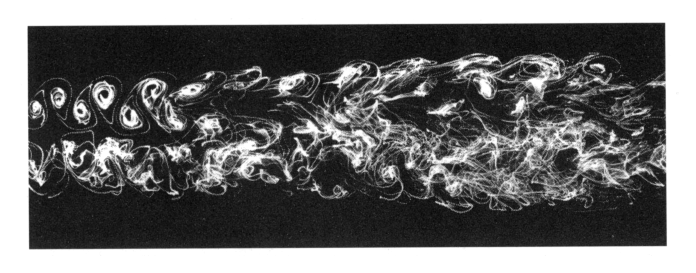
\includegraphics[width=0.7\linewidth]{chapter2/Reynolds240.eps}
	\label{fig:rey240}}
	\subfigure[$Re=1800$]
	{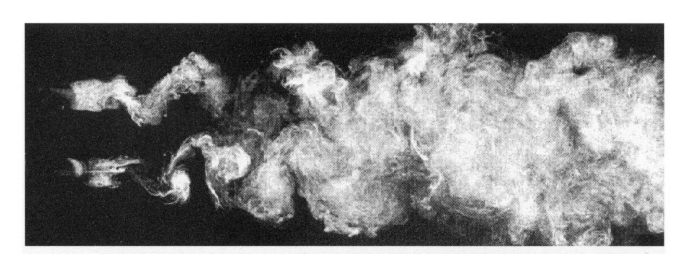
\includegraphics[width=0.7\linewidth]{chapter2/Reynolds1800.eps}
	\label{fig:rey1800}}
	\caption{Wake behind two identical cylinders \citep{Frisch1995}.}
\end{figure}


With increasing Reynolds number,
the left-right symmetry first (figure \;\ref{fig:rey240}) and then the up-down
symmetry are broken (figure \;\ref{fig:rey1800}). If $Re > 1000$, the flow
becomes completely chaotic and all symmetries are broken. Nevertheless, looking
at the flow at smaller scales $l$ far from the boundaries, all the symmetries of
the equations seem to be restored in a statistical sense. This state of flow is
called fully developed turbulence.

However at the smallest scales of the flow $l_k$,
the flow will ``behave'' laminar again. This means that the Reynolds
number becomes smaller on smaller scales and implies that the Reynolds number is
scale dependent
\begin{align}
Re(l)=\frac{\rho v(l) l}{\eta}. 
\end{align}
How the Reynolds number depends on the scales of the flow is explained by the
Kolmogorov theory of incompressible turbulence.

\section{The Kolmogorov theory}\label{kolmo}
Kolmogorov first described his theory of turbulence in 1941. 
Here we discuss the modern formulation of the Kolmogorov theory as
explained in \citet{Frisch1995} and \citet{Pope2000}.

According to Frisch, Kolmogorovs theory is based on three
assumptions which are valid in the limit of infinite Reynolds numbers, at small
scales $l$ $(l_k \ll l \ll l_0)$ and away from boundaries:
\begin{enumerate}
\item All the possible symmetries of
the Navier-Stokes equation, usually broken by the mechanisms producing the
turbulent flow, are restored in a statistical sense.
\item The turbulent flow is self-similar.
\item The turbulent flow has a finite nonvanishing mean rate of dissipation
$\fil{\epsilon}$ per unit mass.
\end{enumerate}
The mean rate of dissipation is defined as the mean rate of change of kinetic
energy
\begin{align}
\fil{\epsilon}=\fil{\td{t}e_{kin}} \sim \frac{v_0^2}{l_0/v_0} =
\frac{v_0^3}{l_0} = const. \label{eq:diss}
\end{align}
Using this Kolmogorov derived, that for homogeneous and isotropic
incompressible turbulence the third order structure function\footnote{For a
definition of structure functions see
appendix \ref{structfunc}.} $S_3(v(l))$ is equal
to the mean rate of dissipation times minus four-fifths the length scale $l$ of
the structure function
\begin{align}
S_3(v(l)) = -\frac{4}{5} \fil{\epsilon} l.
\end{align}
This is the famous four-fifths law of Kolmogorov. From
it and the self similarity assumption, Kolmogorov deduces that the structure
functions of order $p$ scale like
\begin{align}
S_p(v(l)) \sim \fil{\epsilon}^{p/3} l^{p/3}.
\end{align}
Because the second order structure function can be expressed as
Fourier transform of the longitudinal velocity
spectrum\footnote{Also see appendix \ref{structfunc}.} $\abs{V_{\parallel}(k)}^2
\sim e_{kin}(k)$ and the wave numbers $k$ are related to length scales $l$ via
$k \sim l^{-1}$ it follows for the specific kinetic energy in Fourier space
\begin{align}
e_{kin}(k) \sim \fil{\epsilon}^{2/3} k^{-2/3}. 
\end{align}
The energy spectrum $E(k)$ is the kinetic energy in
the wave number interval between $k$ and $k+dk$, which is then
\begin{align}
E(k) \sim \td{k} e_{kin}(k) = C_k \fil{\epsilon}^{2/3} k^{-5/3}.
\end{align}
This is the celebrated result of Kolmogorovs theory of incompressible
turbulence. The constant $C_k$ is therefore called the Kolmogorov constant and
is 
experimentally and numerically found to be $C_k \approx 1.6$
\citep{Yokokawa2002}. 

It should be noted that the rate of dissipation $\fil{\epsilon}$ is not the rate
of conversion of kinetic energy into internal energy, rather it describes the
amount
of energy which is transfered from the bigger to the smaller scales, without
the influence of viscosity. The kinetic energy is converted to internal energy
only on scales smaller than the Kolmogorov scale $l_k$, where the
Reynolds number becomes unity. From this and the relation $S_1(v(l)) \sim v(
l) \sim \fil{\epsilon}^{1/3} l^{1/3}$ we can derive an expression for the
Kolmogorov scale
\begin{align}
Re(l_k) = 1 = \frac{\rho v_{l_k} l_k}{\eta} = 
\frac{\fil{\epsilon}^{1/3} l_k^{4/3}}{\nu} \Rightarrow
l_k = \lra{\frac{\nu^3}{\fil{\epsilon}}}^{1/4}. \label{eq:lk}
\end{align}

Using the definition of the dissipation \eqref{eq:diss} in \eqref{eq:lk}, we
obtain for the ratio between the largest integral length $l_0$ and the
Kolmogorov length $l_k$
\begin{align}
\frac{l_0}{l_k}=\lra{\frac{\nu^3}{l_0^3 v_0^3}}^{-1/4} = Re^{3/4}. 
\end{align}
We can use this to estimate the number of degrees of freedom of a
three-dimensional fluid flow at a point of time
\begin{align}
N_f=\lra{\frac{l_0}{l_k}}^3 = Re^{9/4}.
\end{align}
One consequence of this is that the storage requirement of a fully resolved
numerical simulation grows as $Re^{9/4}$. \footnote{
Using this to estimate the Reynolds number from the biggest direct numerical
simulation today by \citet{Yokokawa2002} on the Earth simulator with a
resolution of $4096^3$ grid cells yields $Re \approx 65536$.} Since the time
step must usually be taken proportional to the spatial mesh, the total number
of operations to integrate the equations for a fixed number of dynamical times
is
\begin{align}
N = \lra{\frac{l_0}{l_k}}^4 = Re^3.
\end{align}
As the typical Reynolds numbers in astrophysical context are of the order of
$10^8$ \citep{Kritsuk2007} up to $10^{14}$ \citep{Schmidt2006} we would
need a computer with at least $10^{18}$ Bytes (1 Exabyte) of memory and
$10^{16}$ FLOPS\footnote{Floating point operations per second.} (10 PetaFLOPS)
running for a year to resolve fully an astrophysical simulation. And even
if we could efficiently make use of the fact, that turbulence is not volume
filling at a
point of time, it remains intractable to resolve completely the turbulent
fluid dynamics encountered in astrophysics \citep{Schmidt2006}.

Therefore we can only treat explicitly a limited number of degrees of freedom,
which correspond to the largest scales of the system. The influence of the
turbulent dynamics from smaller scales onto larger scales has to be treated in a
statistical way. How the dynamics on small scales and the dynamics on large
scales are interconnected, can be seen by explicitly filtering the equations of
fluid dynamics.

  
\chapter{Filter formalism}\label{filter}
Next we present a very general filter formalism, which
is useful when dealing with the compressible equations of fluid dynamics. We
collect the most important rules\footnote{These rules have already been used
implicitely by \citet{Canuto1997,Schmidt2006}, but our work is the first to 
summarize them explicitly.}, which are necessary to filter the compressible
equations of fluid dynamics. 

\section{Reynolds filter}
In general filtering means splitting some quantity $a$ in a mean value $\fil{a}$
generated by the filter procedure and some deviation $a'$ from the mean value.
If a filter fulfills the following relations,
\begin{align}
\fil{A + B} &= \fil{A}+\fil{B},\label{eq:rey1} \\
\fil{C} &= C,\ \text{if $C = $\ const.}, \label{eq:rey2}\\
\fil{\fil{A} B} &= \fil{A} \fil{B}, \label{eq:rey3}
\end{align}
it is called a Reynolds filter or Reynolds operator. From equation
\eqref{eq:rey2} and
(\ref{eq:rey3}) we see that for $B=C=const.$ 
\begin{align}
\fil{\fil{A} C} = \fil{A} C. \label{eq:rey4}
\end{align}
From this relation \eqref{eq:rey4} it follows for $C=1$
\begin{align}
\fil{\fil{A}}=\fil{A}. \label{eq:rey5}
\end{align}
From the last equation (\eqref{eq:rey5}) and \eqref{eq:rey3} we get
for $B=\fil{D}$
\begin{align}
\fil{\fil{A}\fil{D}} = \fil{A}\fil{\fil{D}}=\fil{A}\fil{D}.
\end{align}
If we split a quantity $a$ in a sum of some kind of mean value $\fil{a}$
(computed by a filter
that satisfies the Reynolds criteria \eqref{eq:rey1}-\eqref{eq:rey3}) and some
deviations $a'$
\begin{align}
a=\fil{a}+a'
\end{align}
it follows from equation \eqref{eq:rey5} for the mean of the deviations
\begin{align}
\fil{a'}=\fil{a-\fil{a}}=\fil{a}-\fil{\fil{a}}=\fil{a}-\fil{a}=0.
\label{eq:meandev}
\end{align}
One can show that the so called central moments of this quantity
($\fil{a' b'}$, $\fil{a' b' c'}$, $\fil{a' b' c' d'}$, $\ldots$)
can be expressed in terms of the classical moments  
($\fil{a b}$, $\fil{a b c}$, $\fil{a b c d}$,~$\ldots$)
like\footnote{See for example \citep{Monin1971}.}
\begin{align}
\fil{a' b'}=&\ \fil{a b}-\fil{a}\fil{b}\label{eq:mom2}\\
\begin{split}
\fil{a' b' c'}=&\ \fil{a b c} - \fil{a}\fil{b}\fil{c}\\
&-\fil{a}\fil{b' c'} - \fil{b}\fil{a' c'} - \fil{c}\fil{a' b'}
\end{split}
 \\
\begin{split}
\fil{a' b' c' d'}=&\ \fil{a b c d} - \fil{a}\fil{b}\fil{c}\fil{d}\\
&-\fil{a}\fil{b' c' d'} -\fil{b}\fil{a' c' d'}
-\fil{c}\fil{a' b' d'} -\fil{d}\fil{a' b' c'}\\
&-\fil{a}\fil{b}\fil{c' d'}-\fil{a}\fil{c}\fil{b' d'}-\fil{a}\fil{d}\fil{b'
c'}\\
&-\fil{b}\fil{c}\fil{a' d'}-\fil{b}\fil{d}\fil{a' c'}-\fil{c}\fil{d}\fil{a' b'}
\end{split}
\\
\fil{a' b' c' d' e'} =&\ \ldots \label{eq:mom5}
\end{align}
\section{Germano formalism}
\citet{Germano1992} postulates that the relations between moments and central
moments for non-Reynolds operators\footnote{Non-Reynolds operators do not
fulfill \ref{eq:meandev}, so their mean of the deviations is unequal zero.} are
of similar form as for Reynolds operators.
Therefore he introduces the so called generalized central moments $\tau(a,b), 
\tau(a,b,c),\ldots$ for non-Reynolds operators. These should 
fulfill in analogy to equation \eqref{eq:mom2}-\eqref{eq:mom5} the following
relations\footnote{It seems to be very difficult to prove these relations even
in case of very simple non-Reynolds operators.}
\begin{align}
\tau(a,b)=&\ \fil{a b}-\fil{a}\fil{b} \label{eq:germ2}\\
\begin{split}
\tau(a,b,c)=&\ \fil{a b c} - \fil{a}\fil{b}\fil{c}\\
&-\fil{a}\tau(b, c) - \fil{b}\tau(a, c) - \fil{c}\tau(a, b)\label{eq:germ3}
\end{split}
\\
\begin{split}
\tau(a,b,c,d)=&\ \fil{a b c d} - \fil{a}\fil{b}\fil{c}\fil{d}\\
&-\fil{a}\tau(b, c, d) -\fil{b}\tau(a, c, d)\\
&-\fil{c}\tau(a, b, d) -\fil{d}\tau(a, b, c)\\
&-\fil{a}\fil{b}\tau(c, d)-\fil{a}\fil{c}\tau(b, d)-\fil{a}\fil{d}\tau(b, c)\\
&-\fil{b}\fil{c}\tau(a, d)-\fil{b}\fil{d}\tau(a, c)-\fil{c}\fil{d}\tau(a, b)
\end{split}
\\
\fil{a' b' c' d' e'} =&\ \ldots \label{eq:germ5}
\end{align}
For the generalized central moments the following rules apply:
\begin{enumerate}
\item  They are symmetric in their arguments
\begin{align}
\tau(a,b) = \tau(b,a) ; \tau(a,b,c)=\tau(b,a,c) , \ldots 
\end{align}
\item The generalized central moment of a constant is zero
\begin{align}
\tau(a,c) = 0, \tau(a,b,c) = 0,\ \text{if $c =$ const.}
\end{align}
\item In case of a static (time independent) filter operator 
it permutes with the time derivative and the chain rule applies
\begin{align}
\pd{t}\tau(a,b)=\tau\lra{\pd{t}a,b}+\tau\lra{a,\pd{t}b}
\end{align}
\item If the filter operator is isotropic (independent of 
position in space) then it applies
\begin{align}
\pd{x_i}\tau(a,b)=\tau\lra{\pd{x_i}a,b}+\tau\lra{a,\pd{x_i}b}
\end{align}
\item Additionally the following relation can be proved
\begin{align}
\tau(a,Cb) &= C\cdot \tau(a,b),\ \text{if $C =$ const.} \\
\tau(a,b+c) &= \tau(a,b) + \tau(a,c) \\
\tau(a,bc) &= \tau(a,b,c) + \fil{b}\tau(a,c) + \fil{c}\tau(a,b) 
\end{align}
\end{enumerate}
\section{Favre-Germano formalism} \label{FGform}
In the case of compressible fluid dynamics, the moments appearing in the
filtered equations are one order higher than in non-compressible
fluid dynamics (eg. $\fil{\rho u_i u_j}$ instead of $\fil{u_i u_j}$).
If we would adopt the Germano relations \eqref{eq:germ2} to \eqref{eq:germ5}
in this case, we would get many terms which are difficult to interpret
physically.
But if we use density weighted
quantities\footnote{For a modern review of this procedure
see \citet{Veynante2002}.} similar to \citet{Favre1969} and develop relations in
analogy to the Germano relations for these density weighted
quantities, we can write the filtered compressible equations of fluid dynamics
in a much simpler way \citep{Canuto1997,Schmidt2006}.

We define density weighted quantities according to Favre like
\begin{align}
\fil{\rho a} = \fil{\rho} \hat{a} \Rightarrow \hat{a}=\frac{\fil{\rho
a}}{\fil{\rho}}.
\end{align}
In analogy to Germano we postulate the following relations:
\begin{align}
\hat{\tau}(a,b)=&\ \fil{\rho a b} - \fil{\rho} \hat{a} \hat {b}\\
\begin{split}
\hat{\tau}(a,b,c)=&\ \fil{\rho a b c} - \fil{\rho} \hat{a} \hat{b} \hat{c} \\
&-\hat{a}\hat{\tau}(b,c)-\hat{b}\hat{\tau}(a,c)-\hat{c}\hat{\tau}(a,b)
\end{split}
\\
\hat{\tau}(a,b,c,d)=&\ \ldots
\end{align}
For the quantities $\hat{\tau}(\ldots)$ the same rules apply as for the 
generalized central moments $\tau(\ldots)$ introduced by Germano:
\begin{enumerate}
\item $\hat{\tau}(a,b) = \hat{\tau}(b,a) ; \hat{\tau}(a,b,c)=\hat{\tau}(b,a,c) ,
\ldots$
\item $\hat{\tau}(a,c) = 0, \hat{\tau}(a,b,c) = 0$, if $c =$ const.
\item
$\pd{t}\hat{\tau}(a,b)=\hat{\tau}\lra{\pd{t}a,b}+\hat{\tau}\lra{a,\pd{t}b}$ 
for static filter.
\item
$\pd{x_i}\hat{\tau}(a,b)=\hat{\tau}\lra{\pd{x_i}a,b}+\hat{\tau}\lra{a,\pd{x_i}b}
$
for isotropic filter.
\item
\begin{enumerate} 
\item $\hat{\tau}(a,Cb) = C\cdot \hat{\tau}(a,b)$ , if $C =$ const.
\item $\hat{\tau}(a,b+c) = \hat{\tau}(a,b) + \hat{\tau}(a,c)$ 
\item $\hat{\tau}(a,bc) = \hat{\tau}(a,b,c) + \fil{b}\hat{\tau}(a,c) +
\fil{c}\hat{\tau}(a,b)$
\end{enumerate} 
\end{enumerate}
If we compare the Favre relations to the Germano relations we see:
\begin{align}
\text{Germano:}\ \fil{\rho a} =&\ \fil{\rho}\fil{a} + \tau(\rho,a)\\
\text{Favre:}\ \fil{\rho a}=&\ \fil{\rho}\hat{a}\\
\Rightarrow \hat{a}=&\ \fil{a} + \frac{\tau(\rho,a)}{\fil{\rho}}\\
\Rightarrow \hat{a}=&\ \fil{a},\ \text{if $\rho =$ const.}
\end{align}
This means in the case of a constant density, the formalism with Favre density
weighted quantities
is equivalent to the Germano formalism.
\footnote{This can also be proved for the higher moments.}
\section{Explicit filtering}\label{expfil}
The rules for filtering described in the last sections do not depend on an
explicit form of a filter procedure. However we now want to introduce
a commonly used representation of a filter procedure, namely the convolution
filter. Using a convolution filter the mean value $\fil{a}$ of some
quantity $a(x)$ is defined as 
\begin{align}
\fil{a(x)} = \iinf G(x-x') a(x') dx', 
\end{align}
where $G(x-x')$ is called the convolution kernel, and is associated with
some cutoff length $l_{\Delta}$. The deviation of the mean value is then
defined as
\begin{align}
a' = a(x) - \fil{a(x)} = a(x) - \iinf G(x-x') a(x') dx'.
\end{align}
The importance of the convolution filter stems from the fact that it can be
used to generalise discrete operators, e.g. we can write the well-known
second-order central difference formula for the derivative of a continuous
variable like\footnote{See \citet{Rogallo1984}.}
\begin{align*}
\frac{a(x+h)-a(x-h)}{2h}&=\td{x}\lra{\frac{1}{2h}\int_{x-h}^{x+h} a(x') dx'}\\
&= \td{x} \iinf G(x-x') a(x') dx'\\
&= \td{x} \fil{a}
\end{align*}
with 
\begin{align}
G(x-x') = 
\begin{cases}
\frac{1}{2h} & \text{if }\abs{x-x'} \leq h \\
0 & \text{otherwise}
\end{cases}.\label{eq:box}
\end{align}
The convolution kernel \eqref{eq:box} is also called a box or top-hat filter and
is most often used for performing explicit spatial scale separation. 
   
\chapter{Favre-filtered equations of fluid dynamics}\label{FE}
\section{Basic equations}
Using the Favre-Germano formalism developed in \ref{FGform} to filter the
equations of compressible selfgravitating fluid dynamics
\eqref{eq:mass}-\eqref{eq:etot} leads to

\begin{align}
\pd{t}\fil{\rho} + \pd{r_j}\hat{v}_j\fil{\rho} =&\ 0 \label{eq:film}\\
\pd{t}\fil{\rho}\hat{v}_i + \pd{r_j}\hat{v}_j\fil{\rho}\hat{v}_i =&
-\pd{r_i}\fil{p}+\pd{r_j}\fil{\sigma'_{ij}}+\fil{\rho}\hat{g}_i
-\pd{r_j}\hat{\tau}(v_i,v_j) \label{eq:filmom}
\\
\begin{split}
\pd{t}\fil{\rho}\hat{e}+\pd{r_j}\fil{\rho}\hat{v}_j\hat{e} =&
-\pd{r_j}\fil{v_j p}+\pd{r_j}\fil{v_i \sigma_{ij}}
+\fil{\rho}\hat{v}_i\hat{g}_i\\
&+\hat{\tau}(v_i,g_i)-\pd{r_j}\hat{\tau}(v_j,e)
\end{split}
\end{align}
with
\begin{align}
\hat{e}=\hat{e}_{int}+\frac{1}{2}\hat{v}_i\hat{v}_i
+\frac{1}{2}\frac{\hat{\tau}(v_i,v_i)}{\fil{\rho}}
\end{align}
and
\begin{align}
\hat{\tau}(v_j,e)=\hat{\tau}(v_j,e_{int})+\frac{1}{2}\hat{\tau}(v_j,v_i,v_i)
+\hat{v}_i\hat{\tau}(v_j,v_i)
\end{align}
Filtering the equation for the kinetic energy and the internal energy alone we
get:
\begin{align}
\begin{split}
\pd{t}\fil{\rho} \hat{e}_k+\pd{r_j}\hat{v}_j \fil{\rho} \hat{e}_k) =& 
-\fil{v_i \pd{r_i}p}+\fil{v_i \pd{r_j}\sigma'_{ij}}
+\fil{\rho} \hat{v}_i \hat{g}_i\\
&+\hat{\tau}(v_i,g_i)-\pd{r_j}\hat{\tau}(v_j,e_k) \label{eq:filkin}
\end{split}
\\
\begin{split}
\pd{t}\fil{\rho} \hat{e}_{int}+\pd{r_j}\hat{v}_j \fil{\rho} \hat{e}_{int} =&
-\fil{p \pd{r_j}v_j} + \fil{\sigma'_{ij}\pd{r_j}v_i}
-\pd{r_j}\hat{\tau}(v_j,e_{int})\label{eq:filint}
\end{split}
\end{align}
with
\begin{align}
\hat{e}_k=\frac{1}{2}\hat{v}_i\hat{v}_i
+\frac{1}{2}\frac{\hat{\tau}(v_i,v_i)}{\fil{\rho}}
\end{align}
and
\begin{align}
\hat{\tau}(v_j,e_k)=\frac{1}{2}\hat{\tau}(v_j,v_i,v_i)+\hat{v}_i\hat{\tau}(v_j,
v_i)
\end{align}
\section{Resolved energy and turbulent energy equations}
Multiplying the filtered equation for the momentum (\ref{eq:filmom}) with the
Favre-filtered velocity
$\hat{v}_i$ yields the balance equation for the resolved kinetic energy:
\begin{align}
\begin{split}
\pd{t}\fil{\rho}\frac{1}{2}\hat{v}_i\hat{v}_i 
+ \pd{r_j}\hat{v}_j\fil{\rho}\frac{1}{2}\hat{v}_i\hat{v}_i =&
-\hat{v}_i\pd{r_i}\fil{p}+\hat{v_i}\pd{r_j}\fil{\sigma'_{ij}}
+\fil{\rho}\hat{v}_i\hat{g}_i\\
&-\hat{v}_i\pd{r_j}\hat{\tau}(v_i,v_j) \label{eq:reskin}
\end{split}
\end{align}
Adding the equation for the resolved kinetic energy (\ref{eq:reskin}) to the
equation for the filtered internal energy (\ref{eq:filint}) one gets the
equation for the total resolved
energy $e_{res}=\hat{e}_{int}+\frac{1}{2}\hat{v_i}\hat{v_i}$:
\begin{align}
\begin{split}
\pd{t}\fil{\rho}e_{res}+\pd{r_j}\hat{v}_j\fil{\rho}e_{res}=&
-\hat{v}_i\pd{r_i}\fil{p}+\hat{v}_i\pd{r_j}\fil{\sigma'_{ij}}+\fil{\rho}\hat{v}
_i\hat{g}_i\\
&-\fil{p\pd{r_i}v_i}+\fil{\sigma'_{ij}\pd{r_j}v_i}
-\hat{v}_i\pd{r_j}\hat{\tau}(v_i,v_j)\\
&-\pd{r_j}\hat{\tau}(v_j,e_{int})\label{eq:resetot}
\end{split}
\end{align}
The arising four terms
$\fil{p\pd{r_i}v_i},\fil{\sigma'_{ij}\pd{r_j}v_i},
\hat{\tau}(v_i,v_j),\hat{\tau}(v_j,e_{int})$ in the total resolved energy
represent the coupling of the unresolved fluctuations to the filtered resolved
flow. We could now try to find equations based on quantities of the resolved
flow, to model each of these terms independent of each other.
Nevertheless we will see that the first three of these four terms can be
connected by an equation for another quantity, called the turbulent energy 
$\varepsilon_t$. From solving the equation for this quantity we get the three
terms $\fil{p\pd{r_i}v_i},\fil{\sigma'_{ij}\pd{r_j}v_i},\hat{\tau}(v_i,v_j)$.
Only the fourth term $\hat{\tau}(v_j,e_{int})$ is not connected with the
turbulent energy and has to be modeled separately. 

We get the balance equation for the turbulent energy\footnote{Interpreting the
quantity $\hat{\tau}(v_i,v_i) = \hat{\tau}_{ii}$ as an energy is only possible,
if $\hat{\tau}_{ii} \geq 0$. This is only guaranteed, if the filter 
convolution kernel is a semi-positive function in position
space \citep{Vreman1994,Sagaut2006}.} 
$\varepsilon_t=\fil{\rho} e_t =\frac{1}{2}\hat{\tau}(v_i,v_i)$ by
subtracting the balance equation for the resolved kinetic energy
(\ref{eq:reskin}) from the balance equation of the filtered kinetic energy
(\ref{eq:filkin}) :
\begin{align}
\begin{split}
\pd{t}\fil{\rho}e_t+\pd{r_j}\hat{v}_j \fil{\rho}e_t=&
-\lrb{\fil{v_i \pd{r_i}p}-\hat{v}_i\pd{r_i}\fil{p}} \\
&+\lrb{\fil{v_i \pd{r_j}\sigma'_{ij}}-\hat{v}_i\pd{r_j}\fil{\sigma'_{ij}}} \\
&+\hat{\tau}(v_i,g_i) 
-\frac{1}{2}\pd{r_j}\hat{\tau}(v_j,v_i,v_i) 
-\hat{\tau}(v_j,v_i)\pd{r_j}\hat{v_i}
\end{split}
\end{align}
For a better comparison with \citet{Schmidt2006} we will transform the following
terms like
\begin{align}
\fil{v_i \pd{r_i}p}&=\pd{r_i}\fil{v_i p}-\fil{p \pd{r_i} v_i}
\label{eq:trans1}\\
\hat{v}_i\pd{r_i}\fil{p}&=\pd{r_i}\hat{v}_i\fil{p}-\fil{p}\pd{r_i}\hat{v}_i\\
\fil{v_i \pd{r_j}\sigma'_{ij}}&=\pd{r_j}\fil{v_i \sigma'_{ij}}-\fil{\sigma'_{ij}
\pd{r_j}v_i}\\
\hat{v}_i\pd{r_j}\fil{\sigma'_{ij}}&=\pd{r_j}\hat{v}_i\fil{\sigma'_{ij}}-\fil{
\sigma'_{ij}}\pd{r_j}\hat{v}_i\label{eq:trans4}
\end{align}
and rewrite the balance equation for the turbulent energy:
\begin{align}
\begin{split}
\pd{t}\fil{\rho}e_t+\pd{r_j}\hat{v}_j \fil{\rho}e_t=&
-\pd{r_j}\lrb{\frac{1}{2}\hat{\tau}(v_j,v_i,v_i)+\fil{v_i p}-\hat{v}_i\fil{p}
-\fil{v_i \sigma'_{ij}}+\hat{v}_i\fil{\sigma'_{ij}}}\\
&-\lrb{\fil{p}\pd{r_i}\hat{v}_i-\fil{p \pd{x_i} v_i}} 
+\lrb{\fil{\sigma'_{ij}}\pd{r_j}\hat{v}_i-\fil{\sigma'_{ij} \pd{r_j}v_i}} \\
&+\hat{\tau}(v_i,g_i)-\hat{\tau}(v_j,v_i)\pd{x_j}\hat{v_i}
\end{split}
\end{align}
If we introduce now in analogy to \citet{Schmidt2006} the following
definitions
\begin{align}
-\mu &=\fil{v_i p}-\hat{v}_i\fil{p}\\
-\kappa &=\fil{v_i \sigma'_{ij}}-\hat{v}_i\fil{\sigma'_{ij}}\\
\mathbb{D} &= -\pd{r_j}\lrb{\frac{1}{2}\hat{\tau}(v_j,v_i,v_i) -\mu
+\kappa}\\
\fil{\rho} \lambda &=\lrb{\fil{p}\pd{r_i}\hat{v}_i-\fil{p \pd{r_i}
v_i}}\label{eq:def4}\\
\fil{\rho} \epsilon
&=-\lrb{\fil{\sigma'_{ij}}\pd{r_j}\hat{v}_i-\fil{\sigma'_{ij} \pd{r_j} v_i}}
\label{eq:def5}\\
\Gamma&=\hat{\tau}(v_i,g_i)
\end{align}
we can write the balance equation for the turbulence energy like
\begin{align}
\pd{t}\fil{\rho}e_t+\pd{r_j}\hat{v}_j
\fil{\rho}e_t=\mathbb{D}+\Gamma-\fil{\rho}(\lambda+\epsilon)
-\hat{\tau}(v_j,v_i)\pd{r_j}\hat{v_i}.\label{eq:et2}
\end{align}
With the help of equations (\ref{eq:trans1}) to (\ref{eq:trans4}) and the
definitions 
(\ref{eq:def4}) and (\ref{eq:def5}) we can also rewrite the equation
(\ref{eq:resetot}) for the total resolved energy:
\begin{align}
\begin{split}
\pd{t}\fil{\rho}e_{res}+\pd{r_j}\hat{v}_j\fil{\rho}e_{res}=&
-\pd{r_i}\hat{v}_i\fil{p}
+\pd{r_j}\hat{v}_i\fil{\sigma'_{ij}}+\fil{\rho}\hat{v}_i\hat{g}_i\\
&+\fil{\rho}(\lambda+\epsilon)
-\hat{v}_i\pd{r_j}\hat{\tau}(v_i,v_j)
-\pd{r_j}\hat{\tau}(v_j,e_{int}).\label{eq:resetot2}
\end{split}
\end{align}

\section{Summary}
The last two equations (\ref{eq:et2}) and (\ref{eq:resetot2}) together with
equation 
(\ref{eq:film}) and (\ref{eq:filmom}) (and additionally the Poisson equation for
the gravity term and the equation of state) form a complete system of partial
differential equations for fluid dynamics
\begin{align}
\pd{t}\fil{\rho} + \pd{r_j}\hat{v}_j\fil{\rho} =&\ 0, \label{eq:filmsum}\\
\pd{t}\fil{\rho}\hat{v}_i + \pd{r_j}\hat{v}_j\fil{\rho}\hat{v}_i =&
-\pd{r_i}\fil{p}+\pd{r_j}\fil{\sigma'_{ij}}+\fil{\rho}\hat{g}_i
-\pd{r_j}\hat{\tau}(v_i,v_j),\label{eq:filmomsum}\\
\begin{split}
\pd{t}\fil{\rho}e_{res}+\pd{r_j}\hat{v}_j\fil{\rho}e_{res}=&
-\pd{r_i}\hat{v}_i\fil{p}
+\pd{r_j}\hat{v}_i\fil{\sigma'_{ij}}+\fil{\rho}\hat{v}_i\hat{g}_i\\
&+\fil{\rho}(\lambda+\epsilon)
-\hat{v}_i\pd{r_j}\hat{\tau}(v_i,v_j)
-\pd{r_j}\hat{\tau}(v_j,e_{int}),
\end{split}\label{eq:filresetotsum}
\\
\pd{t}\fil{\rho}e_t+\pd{r_j}\hat{v}_j
\fil{\rho}e_t=&\ \mathbb{D}+\Gamma-\fil{\rho}(\lambda+\epsilon)
-\hat{\tau}(v_j,v_i)\pd{r_j}\hat{v_i}\label{eq:etsum},
\end{align}
where it is often useful to split the equation for resolved energy into an
equation for the resolved kinetic energy and internal energy respectively
\begin{align}
\begin{split}
\pd{t}\fil{\rho} \hat{e}_k+\pd{r_j}\hat{v}_j \fil{\rho} \hat{e}_k) =& 
-\hat{v}_i \pd{r_i}\fil{p}
+\hat{v}_i \pd{r_j}\fil{\sigma'_{ij}}
+\fil{\rho} \hat{v}_i \hat{g}_i\\
&-\hat{v}_i\pd{r_j}\hat{\tau}(v_i,v_j), \label{eq:filkinsum}
\end{split}
\\
\begin{split}
\pd{t}\fil{\rho} \hat{e}_{int}+\pd{r_j}\hat{v}_j \fil{\rho} \hat{e}_{int} =&
-\fil{p} \pd{r_j}\hat{v}_j 
+\fil{\sigma'_{ij}}\pd{r_j}\hat{v}_i
+\fil{\rho}(\lambda+\epsilon)\\
&-\pd{r_j}\hat{\tau}(v_j,e_{int}).\label{eq:filintsum}
\end{split}
\end{align}

The explicit forms of the quantities $\mathbb{D},\lambda,\epsilon,\Gamma$ and
$\hat{\tau}(v_i,v_j)$ are unknown and have to be modeled in terms of the
turbulence energy $e_t$.
The term $\hat{\tau}(v_j,e_{int})$ has to be modeled independently of $e_t$. The
models for all these terms represent our turbulence or subgrid model.


\chapter{LES and SGS model}\label{LES}
\section{The concept of LES}
The idea behind large eddy simulations (LES) is to solve the filtered equations
of fluid dynamics (FE) \eqref{eq:filmsum} - \eqref{eq:etsum} instead of the
unfiltered ones (UE) \eqref{eq:mass}-\eqref{eq:etot}. There are two reasons for
this:
\begin{enumerate}
\item The FE represent a system with a smaller
number of resolved degrees of freedom (DOF) compared with the UE. This is a
necessary restriction, because the numerical discretization itself acts as a
filter\footnote{See section \ref{expfil}.} and limits the number of DOF which we
can resolve in a high Reynolds number flow. In effect this leads to the problem
that the outcome of a simulation of turbulence using the UE depends on the
numerical scheme used. If instead we solve the FE using a certain subgrid model
with a characteristic cutoff length higher than the numerical cutoff length, the
outcome of the turbulence simulation is only dependent on our subgrid model and
not on the numerical scheme used \citep{Mason1999}. From this point of view, we
should call a turbulence model simply a filter model.
\item Using the numerical cutoff as an explicit filter in an energy
conserving numerical scheme converts kinetic into internal energy. But
the back reaction of the internal energy on the kinetic energy can only be 
via the pressure term, which is presumably not right. With an explicit
turbulence model, we can model the backscattering of small scale fluctuations
on the resolved kinetic energy in a much better way \citep{Schmidt2004}. To
model the backscattering we have to know explicitly the amount of energy on the
scales between the cutoff scale and the Kolmogorov scale. This is what we call
subgrid energy or turbulent energy and that is why the term subgrid scale 
(SGS) model is appropriate for the unknown terms in the FE.
\end{enumerate}

Unfortunately there is a substantial variety of SGS models in the literature
and no agreement on a standard model. An extensive overview of SGS models for
incompressible flows can be found for example in the book by \citet{Sagaut2006}.
There are fewer models explicitly for compressible flows. A simple one,
that was first introduced by \citet{Schmidt2004,Schmidt2006a}, will
be described in the next sections. This \emph{Schmidt model}\footnote{Actually
the original implementation of the SGS model proposed by \citet{Schmidt2006a}
had severe problems with energy conservation and was notoriously difficult to
implement in an AMR code. The version of the \emph{Schmidt model} described in
this work is a simplified version, but it conserves energy and proved to be
sufficient for our work.}, together with some
corrections due to \citet{Sarkar1992}, which will be outlined later, is the
model we use to describe the influence of turbulence on the resolved scales
in our work.

\section{Schmidt model} 
As we interpret the trace of the generalized central moment of the
velocity $\fil{\tau}_{ij}$ as a turbulent energy, we can define a
velocity of the turbulent motions\footnote{This is 
based on an analogy to kinetic energy in the sense, that 
$\frac{1}{2}\rho q^2 = \rho e_t$.} $q=\sqrt{2 e_t}$, which is used as
characteristic velocity of the subgrid terms in the Schmidt model. As a
characteristic length scale the size of one grid cell $l_{\Delta}$ is used
\footnote{As mentioned, the implicit cutoff of our subgrid = filter model
should be greater than the numerical cutoff, so one might object, that 
$l_{\Delta}$ is too small for that. But every term in the subgrid model is
multiplied by some dimensionless constant, which is set to a value high enough
to make numerical cutoff effects insignificant.}.

The Schmidt model neglects the convective flux term
$\hat{\tau}(v_j,e_{int})$ and the gravitational effects $\Gamma$ on the subgrid
scales. The models for the other terms are described in the following sections.

\subsection{Transport term \texorpdfstring{$\mathbb{D}$}{D}}
The transport or diffusion term is modeled by a gradient hypothesis, by stating
that the non-linear term is proportional to the turbulent velocity $q^2$
gradient (Kolmogorov-Prandl relation, see \citet[p.97]{Sagaut2006})
\begin{align}
\mathbb{D}=\pd{r_i}C_{\mathbb{D}}\fil{\rho} l_{\Delta} q^2 \pd{r_i} q.
\end{align}
The constant $C_{\mathbb{D}}$ is
calibrated to $C_{\mathbb{D}} \approx 0.4 = \frac{2}{5}$ by
numerical experiments \citep{Schmidt2006}.

\subsection{Pressure dilatation \texorpdfstring{$\lambda$}{lambda}}
For $\lambda$ an estimate is used that is presumably only valid in the
subsonic (nearly incompressible) regime:
\begin{align}
\lambda=C_{\lambda} q^2 \pd{r_i}\hat{v}_i.
\end{align}
The constant $C_{\lambda}=-\frac{1}{5}$ as found by numerical experiments
\citep{Schmidt2006}.

\subsection{Turbulent dissipation
\texorpdfstring{$\epsilon$}{epsilon}}
The turbulent dissipation accounts for effects of viscosity on subgrid scales.
These effects convert turbulent energy to internal energy even if, on the
larger scales, the effect of viscosity can be neglected. The most simple
expression which can be built from the characteristic turbulent velocity and
length scale for the dissipation is
\begin{align}
\epsilon=C_{\epsilon}\frac{q^3}{l_{\Delta}}. \label{eq:epsmodel}
\end{align}
For our simulations we will set $C_{\epsilon}=0.5$.\footnote{Suggested by
W. Schmidt, personal communication.}

\subsection{Turbulence production tensor
\texorpdfstring{$\hat{\tau}(v_i,v_j)$}{tau}}
The turbulence production term is symmetric in its arguments and can
therefore be written as follows
\begin{align}
\hat{\tau}(v_i,v_j)=\hat{\tau}_{ij}=\frac{1}{2}(\hat{\tau}_{ij}+\hat{\tau}_{ij}
)
=\frac{1}{2}(\hat{\tau}_{ij}+\hat{\tau}_{ji}).
\end{align}
By subtracting the trace of this tensor
\begin{align}
\hat{\tau}_{ij}=\frac{1}{2}(\hat{\tau}_{ij}+\hat{\tau}_{ji})
-\frac{1}{n}\delta_{ij}\hat{\tau}_{kk}+\frac{1}{3}\delta_{ij}\hat{\tau}_{kk}
\end{align}
and recognizing that $\hat{\tau}_{kk}=\fil{\rho} q^2 $ we can split the tensor
in a symmetric, tracefree part 
$\hat{\tau}^*_{ij}=\frac{1}{2}(\hat{\tau}_{ij}+\hat{\tau}_{ji})
-\frac{1}{3}\delta_{ij}\hat{\tau}_{kk}$ and the trace
\begin{align}
\hat{\tau}_{ij}=\hat{\tau}^*_{ij}+\frac{1}{3}\delta_{ij}\fil{\rho}q^2 =
\hat{\tau}^*_{ij} + p_t,
\end{align}
where the trace is commonly called turbulent pressure $p_t$.

A model for $\hat{\tau}^*_{ij}$ is based on the turbulent viscosity
hypothesis.
There it is assumed, that $\hat{\tau}^*_{ij}$ is of the same form like
$S^*_{ij}$ for a newtonian fluid, so
\begin{align}
\hat{\tau}^*_{ij}=- 2 \eta_t S^*_{ij}
\end{align}
with a turbulent dynamic viscosity
$\eta_t=\fil{\rho}\nu_t=\fil{\rho}C_{\nu}l_{\Delta} q$ and
\begin{align}
S^*_{ij}=\frac{1}{2}\lra{\pd{r_j}\hat{v}_i+\pd{r_i}\hat{v}_j}
-\frac{1}{3}\delta_{ij}\pd{r_k}\hat{v}.
\end{align}
The turbulence production term is therefore modeled as
\begin{align}
\hat{\tau}(v_i,v_j)=-2\fil{\rho}C_{\nu} l_{\Delta} q
S^*_{ij}+\frac{1}{3}\delta_{ij}\fil{\rho}q^2.
\end{align}

It should be noted, that in general the old idea of turbulent viscosity
(which was first forumlated by \citet{Boussinesq1877}) is
incorrect. As \citet{Pope2000} shows, it
is only true when the ratio of production of turbulent energy
$\Sigma^*=\hat{\tau}^*_{ij}\ppd{r_j}{v_i}$ to dissipation $\epsilon$ is
$\frac{\Sigma^*}{\epsilon}\sim 1$. If this ratio is much greater or much
smaller than one the turbulent viscosity hypothesis is incorrect. 

Nevertheless since it is the most common idea used to model the turbulent
production tensor it is also used in the Schmidt model. Setting the
constant $C_{\nu}=0.05$ seems to be a rational choice \citep{Schmidt2006}.

\subsection{Summary of the Schmidt model}
Using the Schmidt model, the FE form the following system of equations
\begin{align}
\pd{t}\fil{\rho} + \pd{r_j}\hat{v}_j\fil{\rho} =&\ 0,\\
\pd{t}\fil{\rho}\hat{v}_i + \pd{r_j}\hat{v}_j\fil{\rho}\hat{v}_i =&
-\pd{r_i}(\fil{p}+p_t)+\fil{\rho}\hat{g}_i
-\pd{r_j}\hat{\tau}^*_{ij},
\\
\begin{split}
\pd{t}\fil{\rho}e_{res}+\pd{r_j}\hat{v}_j\fil{\rho}e_{res}=&
-\pd{r_i}\hat{v}_i(\fil{p}+p_t)
+\fil{\rho}\hat{v}_i\hat{g}_i\\
&+\fil{\rho}(\lambda+\epsilon)
-\hat{v}_i\pd{r_j}\hat{\tau}^*(v_i,v_j),
)
\end{split}
\\
\pd{t}\fil{\rho}e_t+\pd{r_j}\hat{v}_j
\fil{\rho}e_t=&\ \mathbb{D}-\fil{\rho}(\lambda+\epsilon)
-\hat{\tau}^*(v_j,v_i)\pd{r_j}\hat{v_i}-p_t\pd{r_i}\hat{v_i}.
\end{align}
Again it is often useful to split the equation for resolved energy into an
equation for the resolved kinetic energy and internal energy respectively
\begin{align}
\begin{split}
\pd{t}\fil{\rho} \hat{e}_k+\pd{r_j}\hat{v}_j \fil{\rho} \hat{e}_k) =& 
-\hat{v}_i \pd{r_i}(\fil{p}+p_t)
+\fil{\rho} \hat{v}_i \hat{g}_i
-\hat{v}_i\pd{r_j}\hat{\tau}^*(v_i,v_j),
\end{split}
\\
\begin{split}
\pd{t}\fil{\rho} \hat{e}_{int}+\pd{r_j}\hat{v}_j \fil{\rho} \hat{e}_{int} =&
-(\fil{p}+p_t) \pd{r_j}\hat{v}_j
+\fil{\rho}(\lambda+\epsilon).
\end{split}
\end{align}

\section{Impact of the Schmidt SGS on the fluid equations}\label{ImpactSGS}
\subsection{General observations}
\begin{figure}
\centering
\resizebox{0.7\textwidth}{!}{
%\input{chapter5/energyscheme1.pstex_t}
}
\caption{Energy transfer in the unfiltered equations of fluid dynamics.} 
\label{fig:UE}
\end{figure}

In this section we want to investigate the influence of the Schmidt model on
the equations of fluid dynamics. This can be done most easily in a graphical
way.

One can see in figure \ref{fig:UE} the energy transfer between potential,
kinetic, and internal energy for the UE. We see that it is possible to convert
potential energy into kinetic energy and vice versa, and also kinetic energy
into internal energy and vice versa via adiabatic pressure effects. On the
other side, irreversible changes of state due to viscous effects can only lead
to an increase of internal energy and not(!) vice versa. 

\begin{figure}
\centering
\resizebox{0.7\textwidth}{!}{
%\input{chapter5/energyscheme3b.pstex_t}
}
\caption{Energy transfer in the filtered equations of fluid dynamics with
Schmidt SGS.} 
\label{fig:FE}
\end{figure}

In figure \ref{fig:FE} the energy transfer for the FE with the Schmidt model is
depicted in the same schematical way. We see that the kinetic energy is now
split into two parts:
the filtered kinetic energy on resolved scales and the turbulent energy on
unresolved scales. From this picture it becomes clear that the turbulent energy
is converted to internal energy by the same processes as the filtered kinetic
energy. Also it could be converted to potential energy\footnote{Drawing the
analogy from the conversion of kinetic into internal energy one might ask if
there could be something like irreversible conversion of potential energy into
kinetic energy or perhaps vice versa. But from general relativity we know that
there is no gravity, there is only curvature of space time. It seems very
strange to imagine something like irreversible curvature of space time.}, but as
already
mentioned, this effect is neglected in the Schmidt model and therefore not
depicted here, as well as the effects due to the convective flux term. 

One very important assumption that has not yet been discussed, but is also
depicted in figure \ref{fig:FE}, is that conversion of resolved kinetic energy
into internal energy due to viscous effects is neglected. Basically all SGS
models that make use of the turbulent viscosity hypothesis, and therefore also
the Schmidt model, assume that for high Reynolds numbers the turbulent viscosity
is much greater than the real viscosity. Why this assumption can be made will
be explained in section \ref{dimanalsgs}.

The last conclusion that can be drawn from this pictures is that certain
quantities are related to the cutoff scale ($\Sigma^*,p_t$) and others are
related to the dissipation scale~($\epsilon$,$\lambda$). Nevertheless we find
that the turbulent dissipation $\epsilon$ in the Schmidt model (and also in most
other SGS models) is modeled depending on the cutoff scale $l_{\Delta}$,
although it should ultimately only depend on the dissipation scale. As we shall
see later this is a point of major concern in the development of a SGS
model for an adaptive grid code.
\subsection{Dimensional analysis}\label{dimanalsgs}
In complete analogy to the UE\footnote{See appendix \ref{dimanal}.} we can do a
dimensionless analysis for the FE with the Schmidt model. 
\subsubsection{Momentum equation}\label{dimmom}
Introducing the dimensionless quantities
\begin{align}
e_t^*= \frac{e_t}{q^2_0},\ 
p_t^*=\frac{p_t}{\rho_0 q^2_0},\ 
\tau_{ij}^{**}=\frac{\tau_{ij}}{\eta v_0/l_0}= \frac{\tau_{ij}}{\rho_0 q_0 v_0}
\end{align}
the momentum equation can be written as
\begin{align}
\frac{l_0}{t_0 v_0}\pd{t^*}\fil{\rho^*}\hat{v}^*_i
+\pd{r_j^*}\hat{v}^*_j\fil{\rho^*} \hat { v } ^*_i=&
+\frac{\rho_0 g_0 l_0}{\rho_0 v_0^2}\fil{\rho^*}\hat{g^*}_i
-\frac{p_0}{\rho_0 v_0^2}\pd{r^*_i}\fil{p^*}
-\frac{q_0^2}{v_0^2}\pd{r^*_i}p_t\\
&+\frac{\eta_0}{\rho_0 l_0 v_0 }\pd{r_j^*}\fil{\sigma^{'*}_{ij}}
-\frac{q_0}{v_0}\pd{r^*_j}\hat{\tau}^{**}_{ij}
\end{align}
From this we can estimate, that the turbulent pressure will become important,
when
\begin{align}
\frac{q_0^2}{v_0^2} \geq \frac{p_0}{\rho_0 v_0^2} \Rightarrow
\frac{q_0^2}{p_0/\rho_0} \geq 1
\end{align}
If we now introduce the turbulent Mach number 
\begin{align}
M_t=\frac{q_0}{c_s}
\end{align}
and use $\frac{p_0}{\rho_0} = \frac{c_s^2}{\gamma}$ we see that the turbulent
pressure will dominate over the thermal pressure, if
\begin{align}
M_t^2 \geq \gamma.
\end{align}

The turbulence production tensor $\hat{\tau}^*_{ij}$
becomes important compared to the stress tensor, if
\begin{align}
\rho_0 q_0 l_0 \geq \eta_0.
\end{align}
So we see that if the turbulent viscosity is greater than the physical
viscosity the turbulent production tensor will dominate over the stress tensor 
in the FE. The physical viscosity is
\begin{align}
\eta_0 \sim \rho_0 \sqrt{u_0} l_{\lambda}
\end{align}
where $u_0$ is the mean thermal energy and $l_{\lambda}$ the mean free path of
a particle, so we see that the turbulent viscosity is greater than the
physical viscosity, if
\begin{align}
\frac{q_0^2}{u_0} \geq \lra{\frac{l_{\lambda}}{l_0}}^2 \Rightarrow
\frac{q_0^2}{u_0} \geq \lra{Kn}^2,
\end{align}
which means the ratio of turbulent energy to internal energy must be greater
than the square of the Knudsen number $Kn=\frac{l_{\lambda}}{l_0}$. Since 
in any case the Knudsen number must be much smaller than one for the continuum
approximation to hold, we can practically always assume that the turbulent
production tensor will dominate over the stress tensor.\footnote{Of course this
analysis is restricted to $l_0 > l_k$, since if we resolve the fluid up to the
Kolmogorov length $l_k$ the turbulent energy will be zero. For scales smaller
than the Kolmogorov length we cannot neglect the influence of the physical 
viscosity.} This justifies our
assumption in the Schmidt model to neglect the influence of the stress tensor
completely in the momentum equation and therefore also in the kinetic energy
equation.

For completeness we also compare the gravitational force to the turbulent
pressure, which yields
\begin{align}
\frac{\rho_0 q_0^2}{\rho_0 g_0 l_0} \geq 1. 
\end{align}
Turbulence will thus dominate over gravity in the momentum equation, if the
average turbulent energy is greater than the gravitational energy. 

\subsubsection{Internal energy equation}
The internal energy equation can be analyzed in the same way as the momentum
equation using the additional dimensionless quantities
\begin{align}
e_{int}^*=\frac{e_{int}}{u_0},\ 
\lambda^* = \frac{\lambda}{\lambda_0} = \frac{\lambda}{q_0^2 v_0/l_0},\
\epsilon^* = \frac{\epsilon}{\epsilon_0} = \frac{\epsilon}{q_0^3 /l_0}.
\end{align}
This results in
\begin{align}
\begin{split}
\frac{l_0}{t_0 u_0}\pd{t^*}\fil{\rho^*} \hat{e}_{int}^*
+\pd{r_j^*}\hat{v}_j^* \fil{\rho^*}\hat{e}_{int}^* =&
-\frac{p_0}{\rho_0 v_0^2}\fil{p^*}\pd{r_j^*}\hat{v}_j^*
+\frac{\eta_0 v_0}{\rho_0 u_0 l_0}\fil{\sigma^{'*}}\pd{r_j^*}\hat{v}_j^*\\
&-\frac{q_0^2}{u_0} p_t\pd{r_j^*}\hat{v}_j^*
+\frac{q_0^2}{u_0}\fil{\rho^*}\lambda^*
+\frac{q_0^3}{v_0 u_0}\fil{\rho^*}\epsilon^*.
\end{split}
\end{align}
We see that the pressure dilatation $\lambda$ will dominate over the
pressure term if
\begin{align}
M_t^2 \geq \gamma
\end{align}
and that the turbulent dissipation $\epsilon$ will dominate over the viscous
dissipation, if 
\begin{align}
\rho_0 l_0 q_0 \lra{\frac{q_0}{v_0}}^2 \geq \eta_0 \Rightarrow
\lra{\frac{q_0}{v_0}}^2 \geq \frac{\eta_0}{\eta_t}.
\end{align}
As shown in section \ref{dimmom} $\eta_0 \ll \eta_t$, so we can always neglect
the influence of the stress tensor in the internal energy equation. This also
leads to the conclusion, that turbulence will be the only source of entropy
in the equations, since the only irreversible conversion of energy into
internal energy is via turbulent dissipation $\epsilon$.

\subsubsection{Turbulent energy equation}
For the dimensional analysis of the turbulent energy equation we need the
additional dimensionless quantity
\begin{align}
\mathbb{D}^* = \frac{\mathbb{D}}{\rho_0 q_0^3/l_0}. 
\end{align}
Inserting it together with the dimensionless quantities introduced in the
former sections yields
\begin{align}
\frac{l_0}{t_0 u_0}\pd{t^*}\fil{\rho^*}e_t^*
+\pd{r_j^*}\hat{v}_j^*\fil{\rho^*}e_t^*=&\
\frac{q_0}{v_0}\lra{\mathbb{D}^*-\fil{\rho^*}\epsilon^*}
-\frac{v_0}{q_0}\hat{\tau}^{**}_{ji}\pd{r_j^*}\hat{v_i^*}
-p_t^*\pd{r_i^*}\hat { v_i^* } - \fil{\rho^*}\lambda^*.
\end{align}
This analysis shows that the behavior of turbulent energy equation can be
completely characterized by the ratio $\frac{q_0}{v_0}$. If 
$\frac{q_0}{v_0} \gg 1$, then only diffusion $\mathbb{D}$ and dissipation
$\epsilon$ are relevant. If $\frac{q_0}{v_0} \ll 1$ then the equation is
dominated by the turbulent production term
$\Sigma^*=\hat{\tau}^{*}_{ji}\pd{r_j}\hat{v_i}$ and only if 
$\frac{q_0}{v_0} \approx 1$ do all terms contribute to the equation.

\section{Sarkar model}
The effect of compressibility on the structure of turbulence is an important
but difficult topic in turbulence modeling and is not really taken into account
by the Schmidt model. \citet{Sarkar1992} performed simulations of simple
compressible flows and investigated the influence of the mean Mach number of
the flow on the turbulent dissipation $\epsilon$ and the pressure dilatation
$\lambda$. Based on this analysis he suggested different models for these
terms, which we will describe in the following sections. These modifications
have been proven to yield good results\footnote{See \citet{Shyy1997}.} and
that's why we use them in the course of this work, when we reach the limitations
of the original Schmidt model with our simulations.
 
\subsection{Turbulent dissipation \texorpdfstring{$\epsilon$}{epsilon}}
As a major effect of compressibility from direct numerical simulation
\citet{Sarkar1992} identifies that the growth rate of kinetic energy decreases
when the initial turbulent Mach number increases. This means that the
dissipation of kinetic energy (and therefore also for the turbulent
energy) increases with the turbulent Mach number $M_t$ and
\citet{Sarkar1992} suggests accounting for this effect by using
\begin{align}
\epsilon=C_{\epsilon}\frac{q^3}{l_{\Delta}}(1+\alpha_1 M_t^2)
\end{align}
with $\alpha_1=0.5$ as a model for the dissipation of turbulent energy.

\subsection{Pressure dilatation \texorpdfstring{$\lambda$}{lambda}}
Based on a decomposition of all variables of the equation for instantaneous
pressure\footnote{For a derivation see appendix \ref{diveq}.} 
\begin{align}
\pdd{r_i} p = \pdd{t}\rho- 
\frac{\partial^2}{\partial r_i \partial r_j}(\rho v_i
v_j-\sigma'_{ij})\label{eq:instpres}
\end{align}
into a mean and a fluctuating part and comparisons with direct numerical
simulations of simple compressible flows \citet{Sarkar1992} proposed a different
model for the pressure dilatation 
\begin{align}
\lambda=\alpha_2 M_t \hat{\tau}^*_{ij} \ppd{r_j}{\hat{v}_i} 
- \alpha_3 M_t^2 C_{\epsilon}\frac{q^3}{l_{\Delta}}
- 8 \alpha_4 M_t^2 p_t \ppd{r_k}{\hat{v}_k}
\end{align}
with $\alpha_2=0.15$,$\alpha_3=0.2$ obtained from a curve fit of the model with
DNS simulation. Unfortunately \citet{Sarkar1992} does not specify a value for
$\alpha_4$, so there is some confusion in the literature about it. For example
\citet{Shyy1997} set $\alpha_4 = 0$ and still found the Sarkar model in good
agreement with their DNS simulation. In this work, we adopt a value of 
$\alpha_4 = \alpha_2^2/2$, which was suggested in a work by
\citet{Schmidt2007a}.


\chapter{AMR and LES}\label{amrles}
As mentioned in the last chapter, in LES we try to solve the FE
instead of the UE and treat the unresolved scales with a subgrid scale model,
which acts like a filter with a characteristic length $l_{\Delta}$ for the UE.
However we can only model the subgrid scales in an averaging sense, which can
only be correct, if the fluid motions on the subgrid scales are nearly
isotropic. This limits the LES methodology to flows where we can resolve all
anisotropies, which stem from large-scale features like boundary conditions or
external forces. Therefore the ideal numerical method for LES would include
adaptive gridding to ensure automatically that the grid, and hence the filter,
are everywhere sufficiently fine to resolve the energy-containing motions
\citep[p. 636]{Pope2000}.

\section{Adaptive mesh refinement}\label{amr}
The most powerful technique for grid-based solvers to resolve localized
and anisotropic structures in a flow is adaptive mesh refinement (AMR). 
Using AMR the grid will be refined\footnote{Refined means that the values from a
coarse parent grid are interpolated onto a finer child grid and then
integrated independently from the coarse grid. However, the way how to
interpolate the values from coarse to fine grid is not discussed in the
literature and most often not described by the developers of AMR fluid codes.
Although outside the scope of our work, the dependence of the solution and the
spectrum of the solution on this interpolation routines should be investigated
in the future.}, depending on a refinement criterion, only at
the defined ``interesting'' areas of the flow field. This allows for
treating a much bigger range of dynamic scales of the fluid with the same
number of grid cells compared to a static grid.

\begin{figure}[tp]
\centering
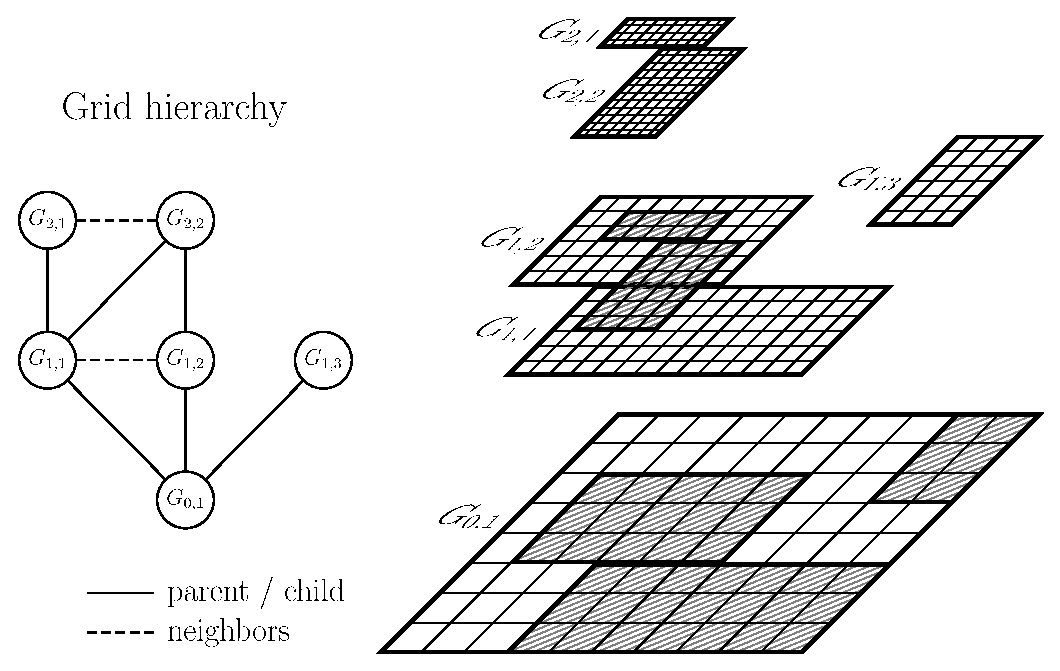
\includegraphics[width=0.7\linewidth]{chapter6/blockamr.eps}
\caption{Hierarchy of rectangular subgrids in blockstructured
AMR \citep{Deiterding2003}.}
\label{fig:amr}
\end{figure}

The grid structure can thereby
be understood as a hierarchy of grid patches (see figure \ref{fig:amr}) that
approximate the flow on various levels of resolution
\citep{Berger1984,Berger1989}. But not only the spatial resolution, also
the time resolution is adaptive. All grids on
a given level are advanced simultaneously with a
maximum timestep such that the Courant condition is
satisfied by all the cells on that level. This results in
a hierarchy of timesteps: a coarse, parent grid on level $l$ is advanced by
$\Delta t^{\text{coarse}}$, and then its finer, subgrid(s) on level $l + 1$ are
advanced by one or more timesteps $\Delta t^{\text{fine}}$ until they reach
the same physical time as their parent grid. 
At this point, the coarse grid values $u^{\text{coarse}}$ are replaced by the
underlying fine grid values $u_i^{\text{fine}}$ using mass weighted,
conservative averaging\footnote{Density itself is not weighted by mass but only
by volume $\rho^{\text{coarse}}=\frac{1}{V}\sum_i \rho_i^{\text{fine}} V_i$.} 
\begin{align}
u^{\text{coarse}}=\frac{1}{M}\sum_i \rho_i u_i^{\text{fine}} V_i,
\end{align}
where $M=\sum_i \rho_i V_i$ is the total mass of the underlying subgrid cells
and $V_i$ is the volume of a fine grid cell. 

To completely ensure mass conservation, however, one not only has to replace the
coarse grid values with averaged fine grid values, but also must correct
coarse grid cells, which abut fine grid cells, but are not themselves
covered by any fine grid. This can be understood, by writing the underlying, 
conservative, explicit finite difference scheme as
\begin{align}
u_n(t+\Delta t^{\text{coarse}}) = u(t) 
- \frac{\Delta t^{\text{coarse}}}{\delta x}
\lra{F^{\text{coarse}}_{n+1/2}-F^{\text{coarse}}_{n-1/2}},\label{eq:finitediff}
\end{align}
where $F_{n \pm 1/2}$ are the fluxes on the left and right hand
side of the cell number $n$ respectively. If the left hand side of cell $n$
abuts on a fine grid, the flux $F^{\text{coarse}}_{n-1/2}$ has to be replaced
by the fluxes of the neighboring fine grid cells
\begin{align}
F^{\text{fine}}_{n-1/2}=\sum_i F_{i+1/2}(t+i \Delta t^{\text{fine}}),
\end{align}
where the sum is due to the refinement in time. This flux replacement is most
often implemented as a correction pass after a grid has been integrated using 
equation \ref{eq:finitediff}
\begin{align}
u_n(t+\Delta t^{\text{coarse,corr}}) = 
u_n(t+\Delta t^{\text{coarse}}) + \Delta F
\end{align}
with 
\begin{align}
\Delta F = -F^{\text{coarse}}_{n-1/2}+
\sum_i F_{i+1/2}(t+i \Delta t^{\text{fine}}).
\end{align}
This "Flux Correction" step is the most difficult and error-prone part of an
AMR implementation, since one has to track all the fluxes of the time varying
boundaries of coarse and fine grids, and correctly maintain them between
processors, if the simulation is run in parallel on several CPUs.   

Nevertheless, if done correctly, this technique has proven to be very well
suited for astrophysical problems which include strong
shocks or gravitational collapse \citep{Bryan2001} among many other
applications. However, in the case of astrophysically relevant Reynolds
numbers\footnote{See section \ref{kolmo}.} even with AMR we cannot hope to
resolve all relevant scales down to the dissipative scales
\citep{Schmidt2006a}.

But as mentioned in the introduction, we do not have to
resolve all scales if we use a SGS model. We only need to resolve
energy-containing motions. That's the reason why combining LES and AMR offers
the
possibility of treating turbulence in astrophysical simulations in a much better
way. Though there is one big problem, when trying to combine LES with AMR. Most
of the terms of a SGS model like the Schmidt model do depend on the
cutoff scale $l_{\Delta}$ of the grid and this cutoff scale varies in time and
space if one uses AMR. But when filtering the fluid dynamic equations, we
assumed our filter operation to commute with time and spatial derivatives and
hence be static and isotropic, in direct contradiction to the methods of AMR.
Therefore combining LES and AMR seem to pose a big challenge and only few
attempts have been made so far.

\section{Attempts to combine LES and AMR}
Although proposals to combine LES and AMR are frequently made
(e.g \citet{Pope2004}), literature on the topic is still rare.

Probably the first attempt to combine LES and AMR is due to
\citet{Sullivan1996}. They used a kind of zero-filling to interpolate
the solution between the coarse and fine grid. But their simulation of
planetary boundary layers only used one static nested fine grid within a coarse
grid and was therefore of limited use for more general problems.
\citet{Boersma1997} came to the conclusion, using the methods of
\citet{Sullivan1996}, that with respect to statistics, the nested grid
simulations are clearly superior to the results obtained with a simulation on a
coarse grid in the whole flow domain. They also found that their
solution of a 2d Kelvin-Helmholtz instability improves even in the area only
covered by the coarse grid, an encouraging fact. Another approach to large eddy
simulations using AMR was put forward by \citet{Cook1999}. He presented a
method for computing a fine grid solution given a coarse grid solution and vice
versa using a deconvolution with a gaussian filter. He showed how to avoid
commutation errors with this technique, and that boundary errors are usually
small. He also emphasized the advantage of using several nested grids instead
of one stretched grid. He came to the conclusion, however, that shocks and
other 
high-frequency phenomena should not be allowed to cross grid boundaries, which
renders his method invalid for simulating compressible flows in astrophysics. 

A sophisticated approach is the multilevel algorithm for large-eddy
simulation of turbulent flow by \citet{Terracol2001,Terracol2003}.
\footnote{Also see the book of \citet{Sagaut2006a}.} But although
they use a time-dependent number of grids, the finer grids in their simulations
always cover the whole computational domain and and are only used to improve
the overall LES performance. Also methods based on wavelets have been proposed
by \citet{Goldstein2004} and \citet{Leonard2006} and even for
adaptive, unstructured grids \citep{Mitran2001a, Naegele2003}, but
seem to be
rarely used. The newest method to combine LES and blockstructured AMR comes from
\citet{Pantano2007}, but they use a very different SGS-model compared to the
Schmidt model considered in our work and therefore it is unclear if their
method is of general use.

Finally in an astrophysical context \citet{Falle1994} claims to use a
$k$-$\epsilon$ subgrid scale model build into the hierarchical adaptive grid
code $\mu$Cobra to treat the effect of turbulence on the large structure of
radio jets. However the specific problems due to adaptive gridding are not
mentioned in this paper and \citet{Falle1994} himself comes to the conclusion
that his treatment of turbulence is rather dubious. Nevertheless, the same model
seems to be used in a recent paper by \citet{Pope2008} on the generation of
optical emission-line filaments in galaxy clusters. 

\section{\texorpdfstring{$\epsilon$}{epsilon}-based approach to combine AMR and
LES}\label{epsilon}
In this chapter, we want to present a new simple method to address the problem
of combination of AMR and LES. It is based on the finding of section
\ref{ImpactSGS}, that the turbulent dissipation $\epsilon$ is related to the
dissipation scale, but in the Schmidt model (and most other SGS models) modeled
depending on the cutoff scale. This is no problem, if we use a static grid in
our fluid dynamic simulation, but it poses a problem in AMR simulations. The
reason is that the time and spatial variance of $l_{\Delta}$ in an adaptive
simulation leads to an artificial dependence of $\epsilon$ on the grid
structure of the simulation. But as we now from Kolmogorovs theory of turbulence
the average rate of dissipation should be independent of the length scale in
fully developed turbulence. This would not be the case in a AMR simulation of
fully developed turbulence, if $\epsilon$ depends on the cutoff scale, since
the average turbulent energy and therefore the turbulent velocity $q$ is 
independent of the lengthscale in a conservative AMR code. So our idea is to
try to enforce the independence of $\epsilon$ on the grid patches of different
cutoff scale in our AMR simulations of turbulence. Explicitely this can be
written as
\begin{align}
\epsilon(l_{\Delta,1})=\epsilon(l_{\Delta,2}),\
l_{\Delta,1} > l_{\Delta,2}
\end{align}
where $\epsilon(l_{\Delta,1})$ is the value of the turbulent dissipation in
one grid cell of the coarse grid and $\epsilon(l_{\Delta,2})$ is the average 
value of the turbulent dissipation after interpolation on a overlapping fine
grid patch.  
Inserting our model for epsilon \eqref{eq:epsmodel} we get
\begin{align}
C_{\epsilon,1}\frac{q_1^3}{l_{\Delta,1}}=
C_{\epsilon,2}\frac{q_2^3}{l_{\Delta,2}}.
\end{align}
Assuming $C_{\epsilon,1}=C_{\epsilon,2}$ this leads to
\begin{align}
\frac{q_1^2}{q_2^2}=\lra{\frac{l_{\Delta,1}}{l_{\Delta,2}}}^{2/3},
\label{eq:qscale}
\end{align}
which is a scaling relation for the turbulent energy. This scaling relation
should hold between the turbulent energy on grid patches of different cutoff
scale. But on the other side, the total energy must be locally conserved
\begin{align}
\frac{1}{2}v_1^2 + \frac{1}{2}q_1^2 + u_1 = 
\frac{1}{2}v_2^2 + \frac{1}{2}q_2^2 + u_2.
\end{align}
Since in a conservative AMR code $u_1 = u_2$ and using the scaling relation
\eqref{eq:qscale} to eliminate $q_2$ we get
\begin{align}
v_2^2=v_1^2+q_1^2 \lra{1-r^{-2/3}},\label{eq:boostekin}
\end{align}
where we introduced the refinement factor
$r=\frac{l_{\Delta,1}}{l_{\Delta,2}}$. 
If we divide \eqref{eq:boostekin} by $v_1^2$ and assume isotropy, we can derive
a relation for the components of velocity 
\begin{align}
v_{2,i}=v_{1,i} \sqrt{1+\frac{q_1^2}{v_1^2} \lra{1-r^{-2/3}}}.
\end{align}
If we write equation \eqref{eq:qscale} like
\begin{align}
q_2^2 = q_1^2 - q_1^2 \lra{1-r^{-2/3}}
\end{align}
we see, that for infinite refinement $r \rightarrow \infty$ the turbulent
velocity  $q_2$ is zero as expected. 


\chapter{Numerical testing}\label{numtest}
\section{The Enzo code}
Enzo is a multiphysics, parallel AMR application for simulating the
cosmological evolution and star formation written in a mixture of C++ and
Fortran, making use of the message-passing interface (MPI) libaries and the 
HDF5 data format. \citet{Norman2007} describes the newest version of the code in
detail. In the following we summarize the most important features of the code.

Enzo simulates the evolution of dark and baryonic matter in a self-consistent
way on cosmological scales. Baryonic matter is evolved using a finite volume
discretization of the compressible fluid dynamic equations in comoving
coordinates\footnote{See appendix \ref{UEcomoving}.}. The Piecewise Parabolic
Method (PPM) in dual energy formalism for high Mach number flows is used to
integrate these equations \citep{Bryan1995}. Energy source and
sink terms due to
radiative heating and cooling processes are included, but not used in our work.
Also we do not use the multi-species (H, H+, He, He+, He++ and e-) capabilities
of Enzo; instead we always set the gas to be fully ionized with a mean
molecular
weight $m_{\mu}= \unit[0.6]{u}$. Dark matter is assumed to behave as
collisionless fluid, obeying the Vlasov-Poisson system of
equations\footnote{See appendix \ref{vlaspois}.}. Its evolution is
solved using particle-mesh algorithms for collisionless N-body dynamics;
specifically a second order accurate Cloud-in-Cell (CIC) formulation with
leapfrog time integration is used. Dark matter and baryonic matter interact
through their
gravitational potential. The gravitational potential is computed by solving the
Poisson equation on the adaptive grid hierarchy using Fast Fourier Transform and
multigrid techniques. In generic terms, Enzo is a fluid solver for the baryonic
matter coupled to a particle-mesh solver for the dark matter via a Poisson
solver. The coordinates of the simulation domain are given as comoving
coordinates in an expanding universe with a scale factor $a(t)$, which is
computed as a solution of the Friedman equation.

The code uses blockstructured adaptive mesh refinement (as described in 
section \ref{amr}) to achieve high resolution. To parallelize the computation,
a concept of ghost grids is used. The root grid is split into a number of grid
patches, at least as many as the number of processors. Then, as grids
are added, each grid is placed by default on the same processor as its parent.
Once the rebuild of the hierarchy has been completed on a given level, the load
balancing ratio between processors is computed and grids are transfered between
processors in an attempt to even the load. However, the structure of the
grid patch hierarchy is stored redundantly on every processor to ease
communication. To allow for this, each real grid, which resides on only one
processor, is represented by a ghost grid (which is a grid patch without data)
on every other processor. This structure is shown graphically in figure
\ref{fig:ghost}. 

\begin{figure}[tp]
\centering
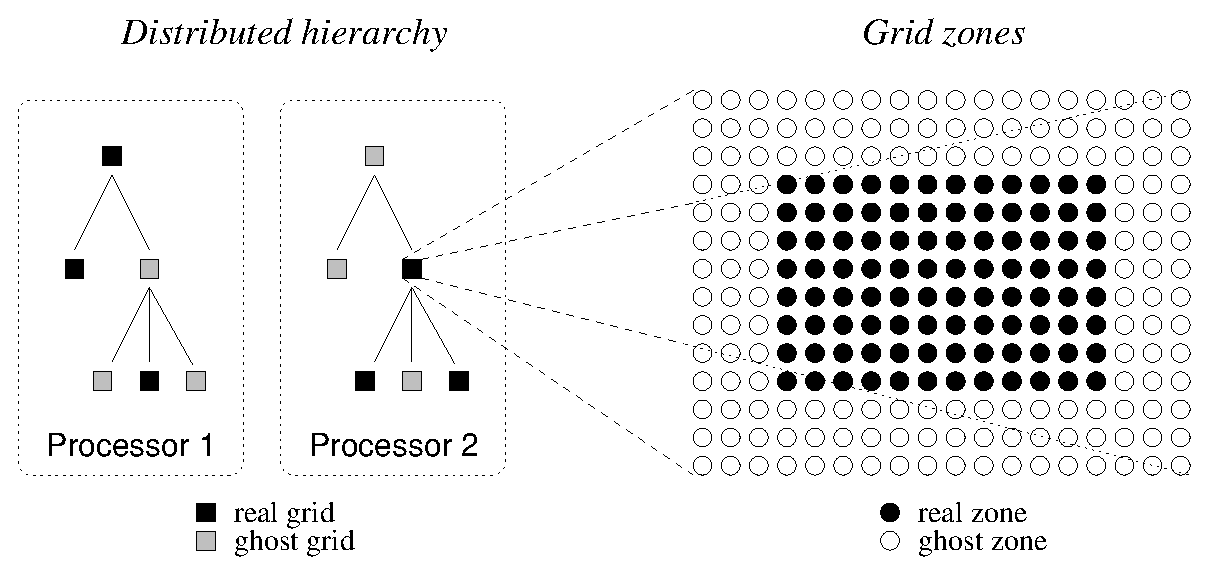
\includegraphics[width=0.7\linewidth]{chapter7/norman-f2.eps}
\caption{Real and ghost grids in a hierarchy; real and ghost zones in a grid 
\citep{Norman2007}.}
\label{fig:ghost}
\end{figure}

Enzo is publicly available from \url{http://lca.ucsd.edu/software/enzo/}.
However to integrate and test our SGS model several modifications to the public
version were necessary.

\section{Modifications to Enzo}
\subsection{Turbulent energy as a color field}
To implement the Schmidt model into Enzo, it was necessary to introduce a new
field for the turbulent energy, which is advected by the PPM solver. To achieve
this, we used the capability of Enzo to incorporate an arbitrary number of
color fields\footnote{See appendix \ref{color}.} into the simulation. Thus the
turbulent energy field is implemented as another color field. Nevertheless it
was necessary to change the default behavior of color fields in Enzo. By
default, Enzo treats a color like a density. But since we want turbulent energy
to be treated in analogy to the internal energy, which is implemented as
specific quantity, we changed the treatment of color fields in our version of
Enzo as to behave like a specific quantity.

\subsection{Coupling of turbulent energy and time step restriction}
The source/sink terms in the turbulent energy equation and the terms arising in
the internal energy equation and the momentum equation due to our subgrid model
are coupled to the fields in first order, which means for some arbitrary field
$f$ at timestep $t_n$, the source terms $s_1,s_2, \ldots$ are added in the
following way 
\begin{align}
f_{n+1} = f_n + s_{1,n} \Delta t + s_{2,n} \Delta t + \ldots
\end{align}
where $\Delta t = t_{n+1}-t_n $ is the chosen timestep. But due to the low
accuracy of the scheme, it might happen, that for a big timestep the value of
one of the energy fields in a cell drops below zero, which is unphysical and
numerically unstable. To account for that, we had to restrict the timestep in
the code. We do this by applying the following estimator
\begin{align}
\Delta t_{turb} = C_{turb} 
\min \lra{\sqrt{\frac{l_{\Delta}}{\abs{\vec{a}_{turb}}}}},
\end{align}
where the minimum is taken over all cells of all grids on one
level of refinement, the turbulent acceleration is $\vec{a}_{turb}=
\frac{1}{\fil{\rho}}{\pd{r_j}\hat{\tau}(v_i,v_j)}$ and $C_{turb} = 0.05$. If
the so-estimated minimal allowed timestep due to our turbulent model $
\Delta t_{turb}$ is smaller than the timestep computed by the other estimators
in the code (e.g. estimator based on the CFL-criterion, for gravity and so on) 
it will be chosen as the timestep for the next iteration. This procedure
ensures that even for big turbulent acceleration (which also means
big source/sink terms) due to our turbulent model, our computation is
numerically stable. Of course, there is one drawback to this procedure: if the
turbulent acceleration becomes really huge, the timestep of the simulation will
be extremely small, effectively stopping the simulation. This can only be
circumvented by either using a higher accuracy scheme for coupling the 
sink/source terms to the equations or by using a different subgrid model, which
does not produce numerically instable huge values of $\abs{\vec{a}_{turb}}$.
The Sarkar corrections are a step in this direction, but further steps may be
necessary in the future. 

\subsection{Transfer of turbulent energy at grid refinement/derefinement}
By default, when a new finer grid gets created in Enzo, the values on the finer
grid are generated by interpolating them from the coarser grid using a
conservative interpolation scheme. At each timestep of the coarse grid, the
values from the fine grid are averaged and replace the values computed on the 
coarse grid in the region where fine and coarse grid overlap. As already
mentioned in section \ref{epsilon} these procedures must be modified in our
approach to combine LES and AMR.

So at refinement we do the following:
\begin{enumerate}
\item Interpolate the values from the coarse to the fine grid using standard
interpolation scheme from Enzo.
\item On the finer grid, correct the values of specific kinetic energy 
$e_k= \frac{1}{2}v^2$, velocity components $v_i$ and specific turbulent energy
$e_t=\frac{1}{2}q^2$ as follows
\begin{align}
e'_k&=e_k+e_t \lra{1-r^{-2/3}},\\
v'_i&=v_i \sqrt{1+\frac{e_t}{e_k}\lra{1-r^{-2/3}}},\\
e'_t&=e_t-e_t\lra{1-r^{-2/3}},
\end{align}
where primed quantities are the final values on the fine grid.
\end{enumerate}

At derefinement we reverse this procedure:
\begin{enumerate}
\item Average the values from the fine grid and replace the corresponding values
on the coarse grid
\item On the coarse grid, correct the averaged values of kinetic energy, 
velocity components and turbulent energy
\begin{align}
e'_t&=e_t+e_t\lra{r^{2/3}-1},\\
v'_i&=v_i \sqrt{1-\frac{e_t}{e_k}\lra{r^{2/3}-1}},\\
e'_k&=e_k-e_t \lra{r^{2/3}-1}.
\end{align}
Here primed quantities denote the final values on the coarse grid. 
\end{enumerate}
It should be noted that derefinement with this procedure is only possible if
there is enough kinetic energy on the fine grid, because on the coarse grid, we
must have $e'_k \geq 0$. This is only the case for
\begin{align}
\frac{e_t}{e_k} \leq \lra{r^{2/3}-1}.
\end{align}
For example for a refinement ratio $r=2$ this yields $e_k \geq 0.58 e_t$.
So if this criterion is not satisfied, we do not correct the values of the
energies and velocities at derefinement.\footnote{One might ask, why not do
the correction step before the interpolation/averaging step, since that might
produce less noise. The reason for our choice was, that otherwise we would had
to introduce an additional temporary field into the code, which would lower
the performance.}

\subsection{Random forcing}\label{randforce}
To simulate driven turbulent flow, a random forcing mechanism was implemented
into our version of Enzo. The forcing field is generated by a stochastic
differential equation called Ornstein-Uhlenbeck process
\citep{Schmidt2004}. This 
process generates a temporally and spatially varying force field which acts on
the fluid. The components of the force are generated in Fourier space, because
there it is easier to split the force field into a solenoidal and a 
dilatational (compressive) part.\footnote{Also called Helmholtz decomposition,
see \citet{Schmidt2004}.} Hence the force field is characterized by a weight
$\zeta$, which is zero, if the force field is purely compressive (which means it
will not directly generate any vorticity), and one, if the force field
is purely solenoidal (which means it will not directly generate any
divergence in the velocity field). The strength of the force field is
characterized by a forcing 
Mach number $M_f$, which is loosely connected to the mean Mach number reached 
in the simulation after one integral time
\begin{align}
t_{int}=\frac{l_0}{M_f \fil{c_s}},
\end{align}
where $l_0$ is the mean driving length scale size and
$\fil{c_s}$ is the mean sound speed. The force field is adjusted to drive
the fluid only on length scales around the characteristic forcing length $l_0 =
\frac{l_{box}}{\alpha_f}$ with $\alpha_f =2 $ to allow for an
undisturbed generation of the energy dissipation cascade down to smaller
scales. 

\subsection{Statistics tool}
To be able to extract and analyze statistical quantities from the simulation,
sophisticated routines have been implemented, which allow us to compute 
mass weighted and normal mean values, standard deviations and root mean square
values at every cycle for each quantity and for each level of an AMR simulation.
We make heavy use of these routines in the following sections. 

\section{Energy conservation}\label{numenergy}
Global conservation of energy in a fluid code with a SGS model like the
Schmidt model is not achieved easily. This is because of the nonlocal features
of this model. As shown in chapter \ref{FE}, the equation of turbulent energy
\eqref{eq:etsum} is generated by subtracting the equation of resolved kinetic
energy \eqref{eq:filkinsum} from the filtered equation of turbulent energy
\ref{eq:filkin}. In other words, the sum of turbulent energy equation and
resolved energy equation must yield the filtered kinetic energy equation.
In particular, the sum of turbulent production term
$\hat{\tau}(v_j,v_i)\pd{r_j}\hat{v_i}$ and resolved kinetic energy reduction
term $\hat{v}_i\pd{r_j}\hat{\tau}(v_i,v_j)$ must add
up to the corresponding flux term in the filtered equation of kinetic energy
\begin{align}
\pd{r_j}\hat{v}_i\hat{\tau}(v_i,v_j) =
\hat{v}_i\pd{r_j}\hat{\tau}(v_i,v_j)+\hat{\tau}(v_j,v_i)\pd{r_j}\hat{v_i}.
\label{eq:fluxsum}
\end{align}
This is important, since we know that the integral of the flux term over the
whole volume must be zero
\begin{align}
\int \pd{r_j}\hat{v}_i\hat{\tau}(v_i,v_j) dV = 
\oint\hat{v}_i\hat{\tau}(v_i,v_j) dA = 0. \label{eq:globalflux}
\end{align}
But this is not guaranteed numerically, if we compute the turbulent production
term and the kinetic energy reduction term independent of each other, since
small numerical errors might lead to a violation of equation \eqref{eq:fluxsum}
locally, which leads to a big violation of equation \eqref{eq:globalflux}
globally.

We therefore compute the resolved kinetic energy reduction term indirectly as
\begin{align}
\hat{v}_i\pd{r_j}\hat{\tau}(v_i,v_j) = 
\pd{r_j}\hat{v}_i\hat{\tau}(v_i,v_j) - 
\hat{\tau}(v_j,v_i)\pd{r_j}\hat{v_i},
\end{align}
since this will guarantee, that equation \eqref{eq:globalflux} is fullfilled
globally. We found that the global energy is thus much better conserved. 

In the following we present our results on energy conservation. The analyzed
simulation of driven turbulence has a static grid of size 1.0 (in code units)
with a resolution of $256^3$ grid points and periodic boundary conditions. At
time $t=0$ the baryonic fluid is at rest. The fluid is driven by random forcing
as described in section \ref{randforce} with $\zeta = 1.0$ and $M_f = 0.68$. The
simulation is adiabatic (the adiabatic index $\gamma=\frac{5}{3}$) and uses none
of the features
necessary for a cosmological simulation (comoving coordinates, selfgravity, dark
matter \ldots) except dual energy formalism. The mean sound speed of the
simulation is $c_s=\sqrt{\gamma}$, since the mean pressure and density are set
to one in code units. 

\begin{figure}[tp]
\centering
\subfigure[No SGS model.]{
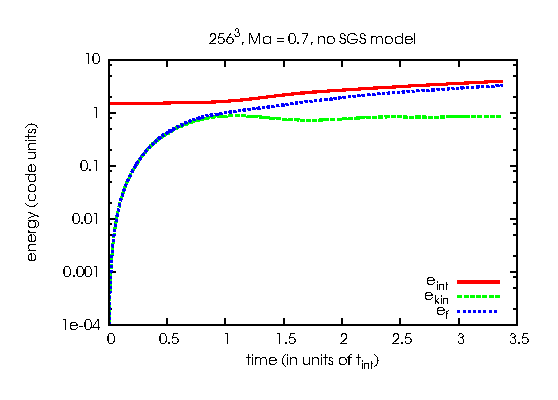
\includegraphics[width=0.45\linewidth]{chapter7/energynosgs2.eps}
\label{fig:nosgs}}
\subfigure[Schmidt model.]{
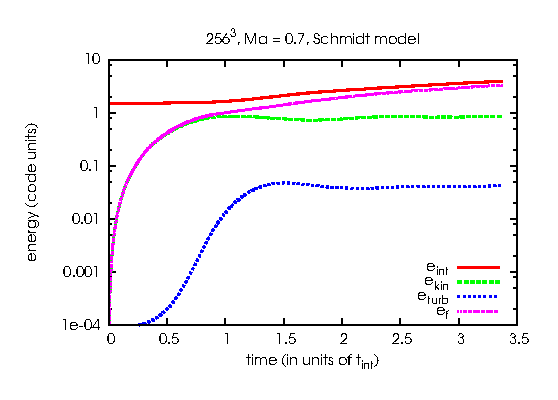
\includegraphics[width=0.45\linewidth]{chapter7/energysgs2.eps}
\label{fig:sgs}}
\caption{Mass weighted mean energies over time in driven turbulence simulation.}
\end{figure}

The plots \ref{fig:nosgs} and \ref{fig:sgs} show the typical time development of
the mass weighted mean energies in our simulation including the energy injected
into the system by random forcing. It is evident from the curve of the turbulent
energy, that after one integral time scale, our simulation reaches a equilibrium
between production and dissipation of turbulent energy.

\begin{figure}[tp]
\centering
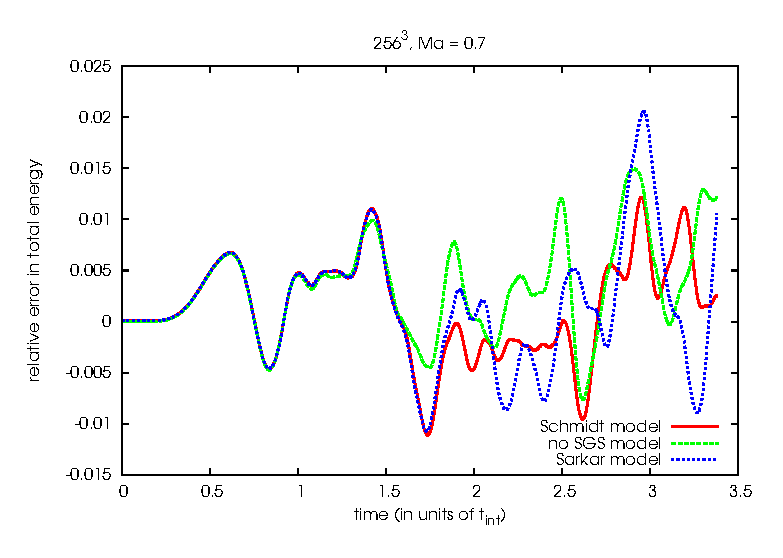
\includegraphics[width=0.7\linewidth]{chapter7/relerror2.eps}
\caption{Relative error of total energy in the simulation.}
\label{fig:relerror}
\end{figure}

In figure \ref{fig:relerror} we plotted the time development of the relative
error $\frac{\Delta e(t)}{e(0)}$ of the mean total energy,
which is the sum of the mass weighted means of internal energy, kinetic energy,
turbulent energy minus the injected energy due to the forcing
\begin{align}
\hat{e}_{tot}= \hat{e}_{int}+\hat{e}_{kin}+\hat{e}_t-\hat{e}_f, 
\end{align}
where $\hat{e} = \frac{\fil{\rho e}}{\fil{\rho}}$. It demonstrates, that with
our Schmidt model, the relative error in energy is comparable to the error
without SGS model and is around 1\%. Also the energy conserving properties of
the Sarkar model are equally good. 

\begin{figure}[tp]
\centering
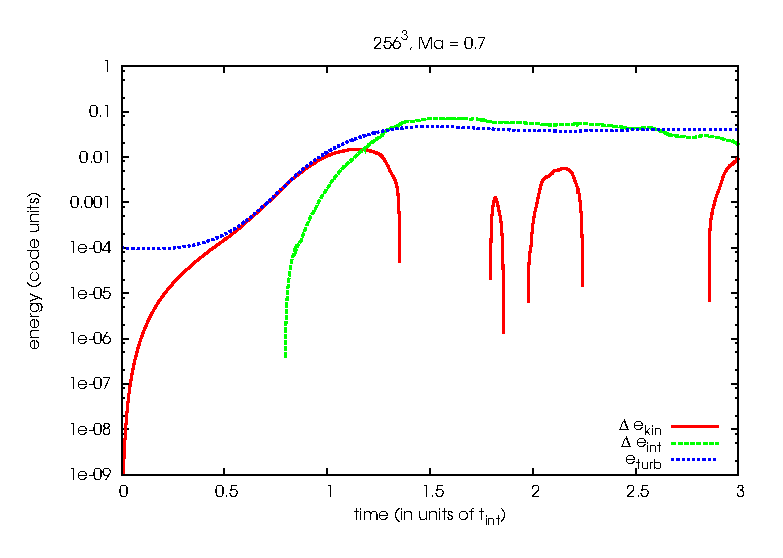
\includegraphics[width=0.7\linewidth]{chapter7/diffenergy2.eps}
\caption{Differences in energies between simulation with and without SGS model,
compared to the time development of the turbulent energy.}
\label{fig:diffenergy}
\end{figure}

It is also instructive to plot the difference between internal energy of the
simulation without the SGS model and the internal energy with the Schmidt model
and the
difference between the kinetic energies of both simulations. These differences
are shown in figure \ref{fig:diffenergy}. One can conclude from this figure,
that, at the beginning of the turbulent driving, the turbulent energy produced
in our simulation with SGS is found in the kinetic energy of the
simulation without SGS. From $t=1.2\ t_{int}$ on most of the turbulent energy
can be found in the internal energy of the simulation without SGS.
Turbulent energy can therefore be interpreted as a kind of buffer, which
prevents the kinetic energy in our simulation to be converted instantly into
thermal energy.  

\section{Scaling of turbulent energy}\label{eturbscale}
In our $\epsilon$-based approach to combine AMR and LES we assumed that the
turbulent energy scales according to equation $\eqref{eq:qscale}$ like
$q^2 \sim l^{2/3}$. We conducted several simulations of driven turbulence to
check the validity of this assumption.

The simulations were done on a static grid in a computational domain of size
1.0 with periodic boundary conditions. At
time $t=0$ the baryonic fluid is at rest. The fluid is driven by random forcing
as described in section \ref{randforce} with $\zeta = 0$ (purely solenoidal
forcing). The simulations were done for nearly isothermal gas
($\gamma=1.01$) with mean pressure and density set to $1.0$ in code units.
We used forcing Mach numbers of $M_f=0.2$ and $M_f=0.68$ and varied the
resolution from $32^3$ to $256^3$ grid points. For $M_f=0.68$ the simulations
were transonic reaching reaching a Mach number around one (see figure
\ref{fig:mach}).

\begin{figure}[tp]
\centering
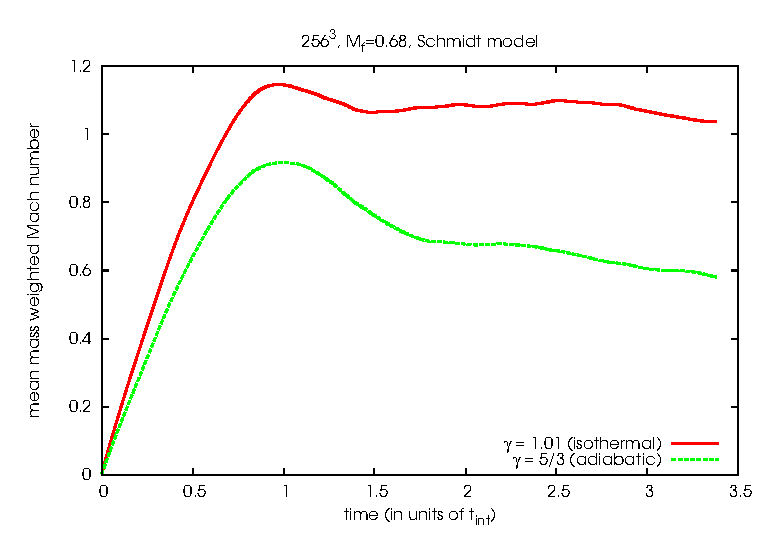
\includegraphics[width=0.7\linewidth]{chapter7/mach2.eps}
\caption{Mean Mach number for adiabatic and isothermal simulation using an
equal
forcing Mach number $M_f=0.68$.}
\label{fig:mach}
\end{figure}

The characteristic time development of the turbulent energy dependent on the
resolution of the simulation can be seen in figures \ref{fig:mf2schmidt} -
\ref{fig:mf7sar}. 

\begin{figure}[tp]
\centering
\subfigure[Schmidt model, $M_f=0.2$.]{
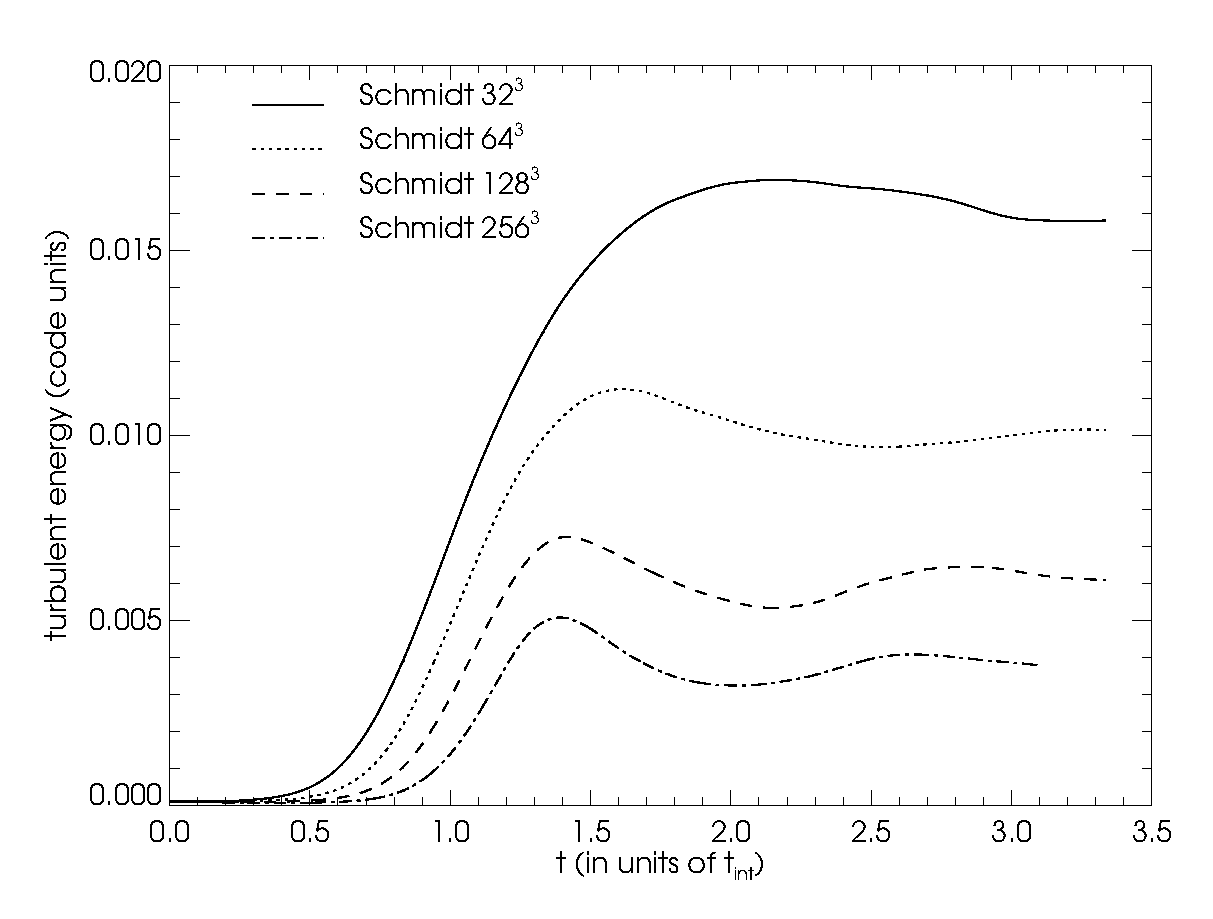
\includegraphics[width=0.45\linewidth]{chapter7/tueres2schmidt.eps}
\label{fig:mf2schmidt}}
\subfigure[Sarkar model, $M_f=0.2$.]{
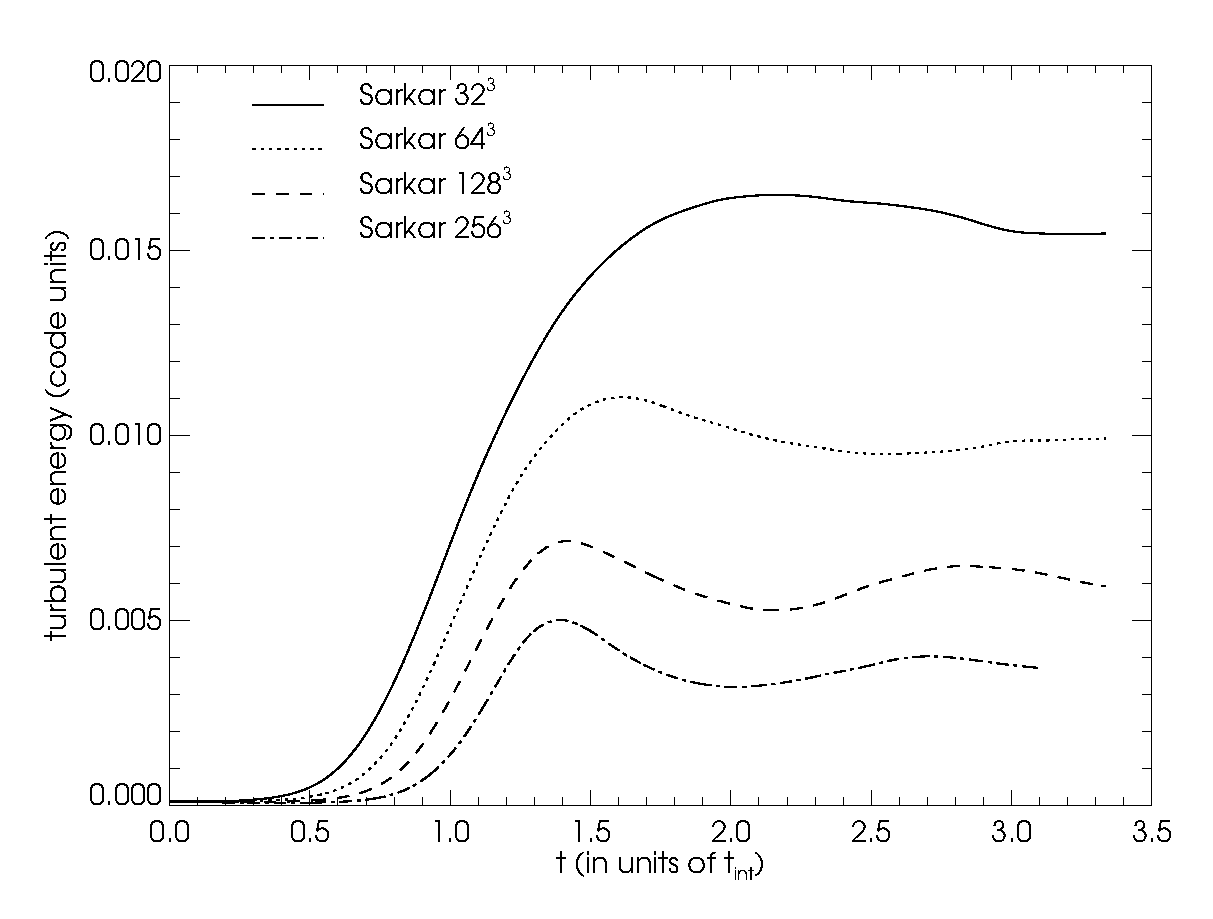
\includegraphics[width=0.45\linewidth]{chapter7/tueres2sar.eps}
\label{fig:mf2sar}}
\subfigure[Schmidt model., $M_f=0.7$]{
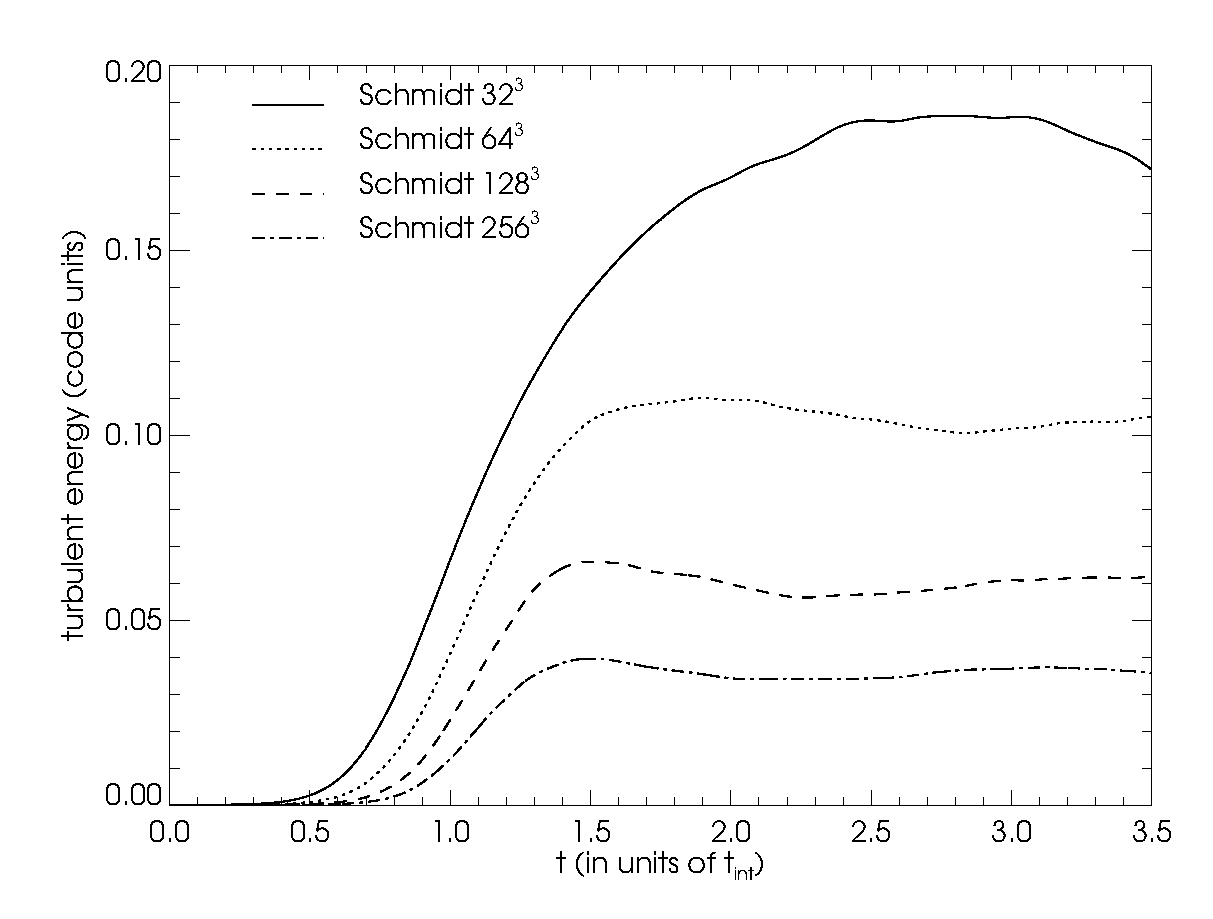
\includegraphics[width=0.45\linewidth]{chapter7/tueres7schmidt.eps}
\label{fig:mf7schmidt}}
\subfigure[Sarkar model, $M_f=0.7$.]{
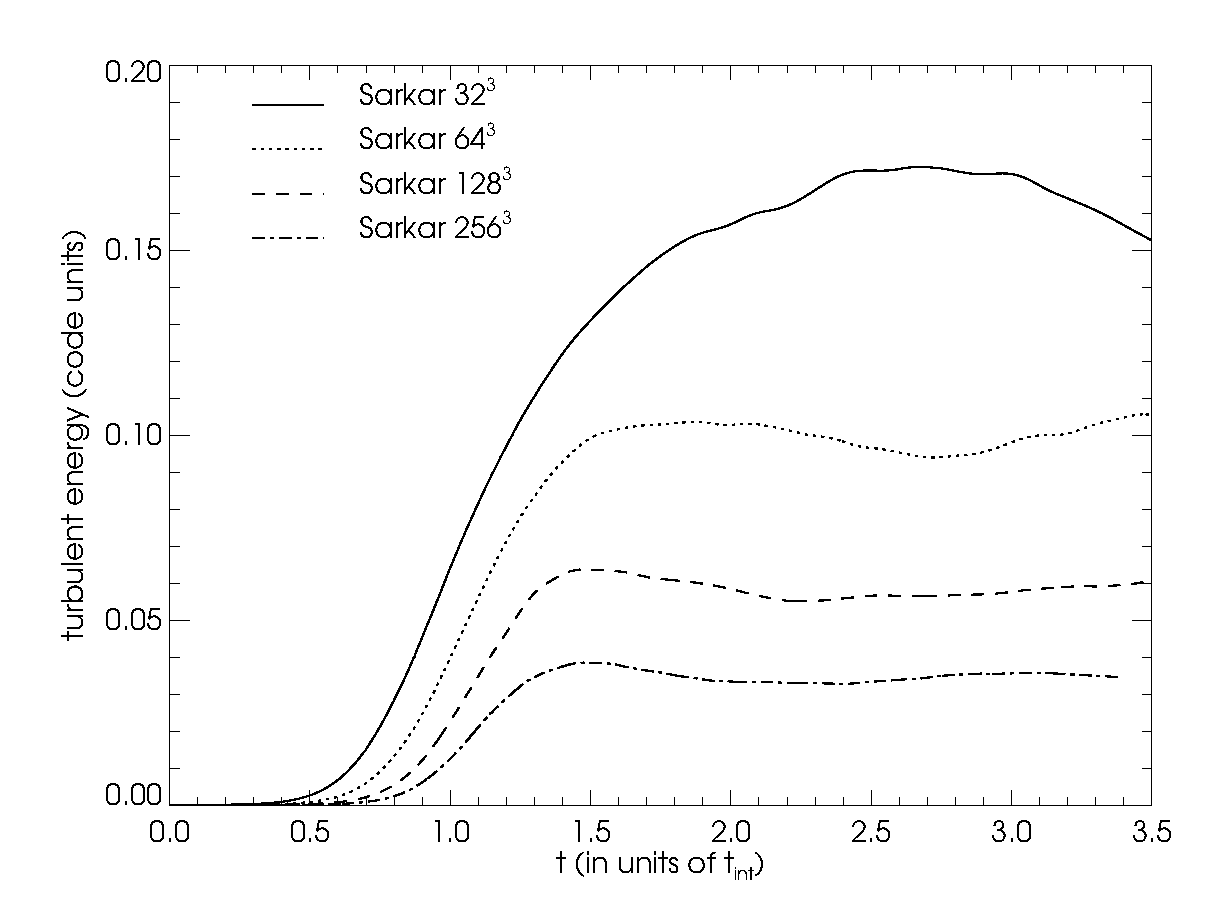
\includegraphics[width=0.45\linewidth]{chapter7/tueres7sar.eps}
\label{fig:mf7sar}}
\caption{Mass weighted mean turbulent energies over time in driven turbulence
simulation, for resolutions $32^3$ to $256^3$ with forcing Mach number $M_f=0.2$
and $M_f=0.68$.}
\end{figure}

We compute mean turbulent energies by
averaging the turbulent energy from $t=3.0\ t_{int}$ to the end of the
simulation
and plot them against the resolution of the simulation. The results together
with a power-law fit are shown in figures \ref{fig:tuefit2} and
\ref{fig:tuefit7}. 
From this we see that for a low Mach number forcing our assumption  
$q^2 \sim l^{2/3}$ ($l$ is indirect proportional to the resolution) is fulfilled
indeed. Nevertheless for high Mach number flows the scaling of turbulent energy
becomes steeper and is $q^2 \sim l^{0.77}$ for the Schmidt model and 
$q^2 \sim l^{0.71}$ for the Sarkar model. In other words for
higher Mach number flows, our correction of turbulent energy at grid 
refinement/derefinement based on relation $\eqref{eq:qscale}$ should probably
be seen only as a good guess of the initial values of turbulent energy on
the finer/coarser grid. Also we conclude that for higher Mach number flows one
should use the Sarkar corrections to the Schmidt model, since this leads
to a scaling of turbulent energy more similar to the incompressible low Mach
number case. 

\begin{figure}[tp]
\centering
\subfigure[$M_f=0.2$.]{
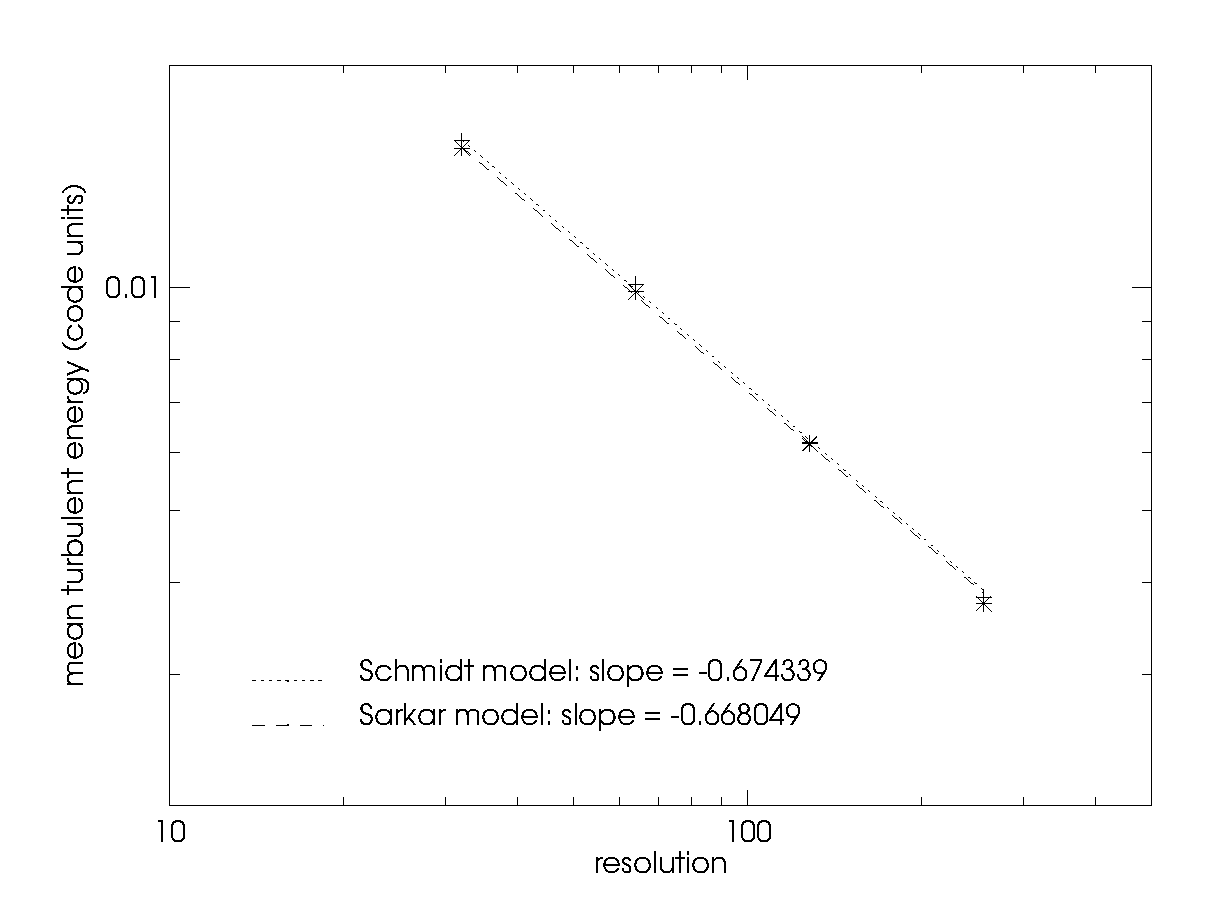
\includegraphics[width=0.45\linewidth]{chapter7/tuefit2.eps}
\label{fig:tuefit2}}
\subfigure[$M_f=0.68$.]{
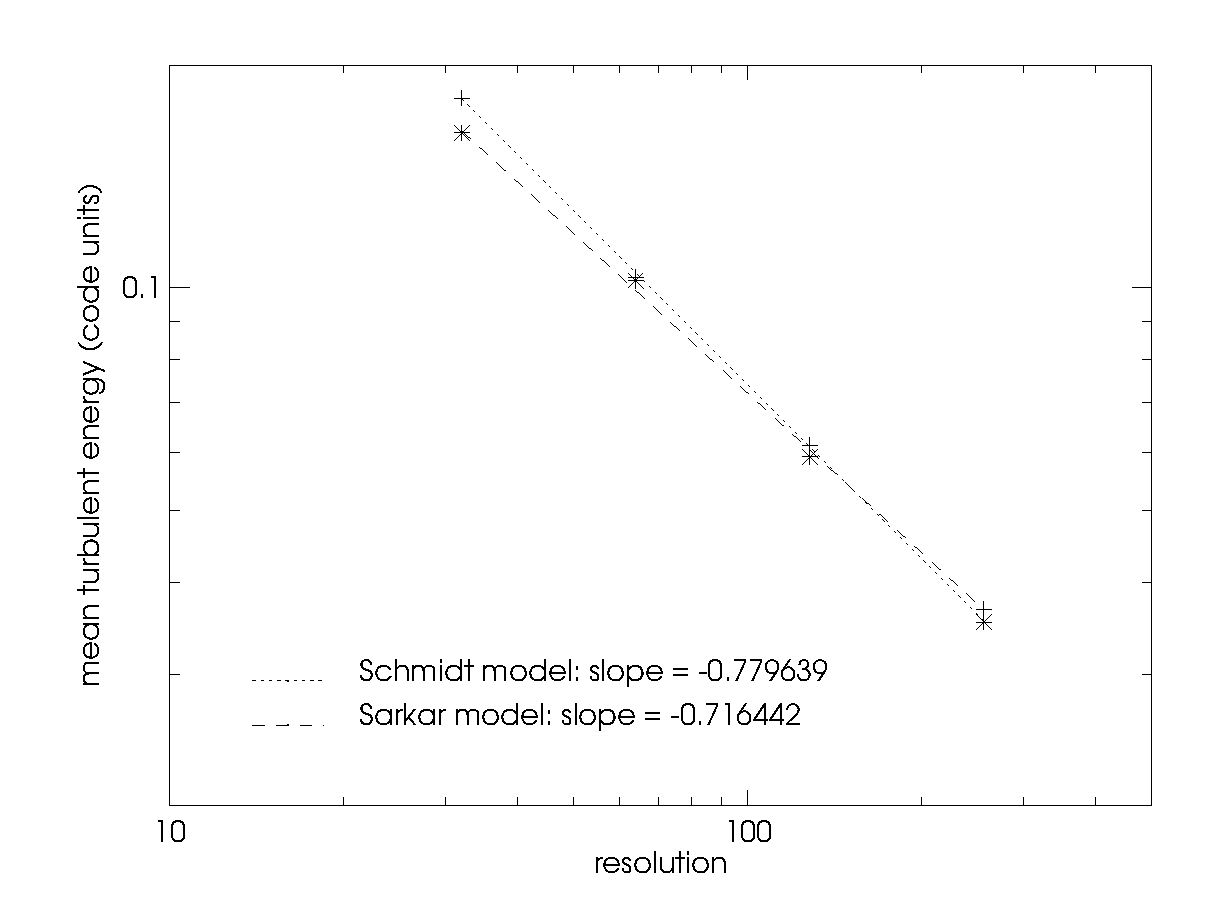
\includegraphics[width=0.45\linewidth]{chapter7/tuefit7.eps}
\label{fig:tuefit7}}
\caption{Scaling of turbulent energy dependent on resolution for different
strength of the forcing.}
\end{figure}

\section{Comparison of static grid to AMR turbulence simulations}

\begin{figure}[p]
\centering
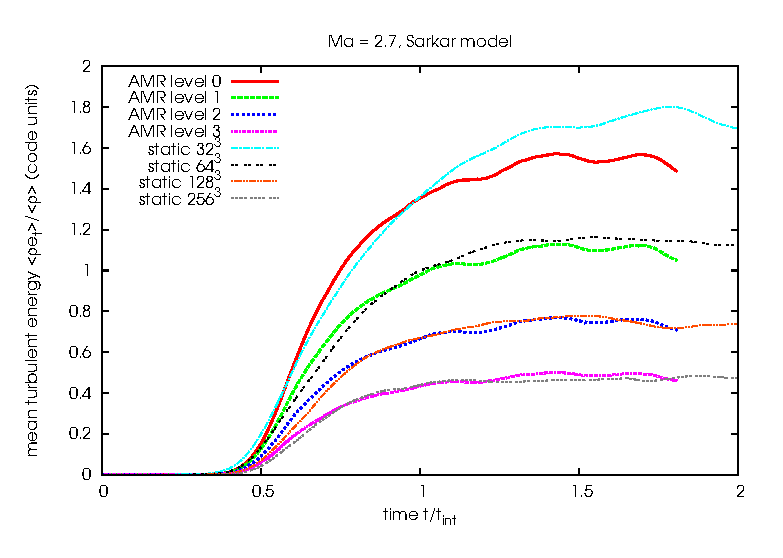
\includegraphics[width=0.7\linewidth]{chapter7/eturbamr27trs2sar.eps}
\caption{Thick lines: mean mass weighted turbulent energy for each level of the
 AMR simulation using our procedure of transferring turbulent energy at grid
refinement/derefinement. Thin lines: the corresponding development of turbulent
energy of the static grid simulations.}
\label{fig:amrtrs2}
\end{figure}

\begin{figure}[p]
\centering
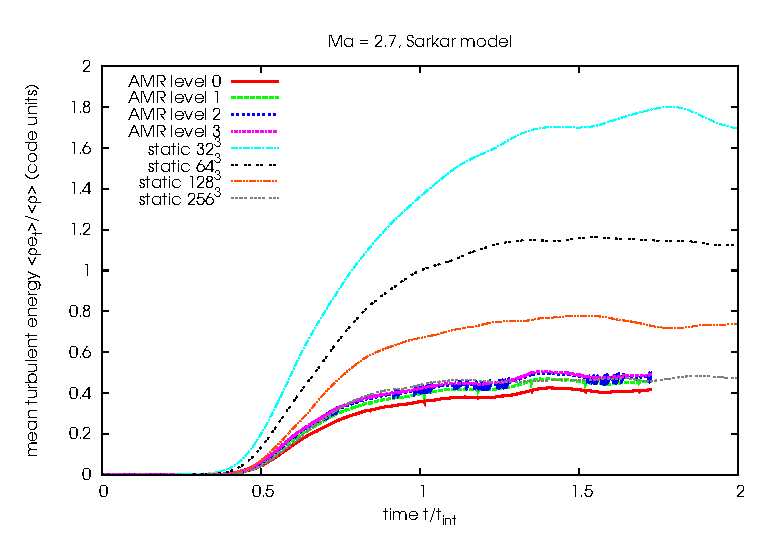
\includegraphics[width=0.7\linewidth]{chapter7/eturbamr27trs0sar.eps}
\caption{Thick lines: mean mass weighted turbulent energy for each level of the
 AMR simulation without transferring turbulent energy at grid 
refinement/derefinement. Thin lines: the corresponding development of turbulent
energy of the static grid simulations.}
\label{fig:amrtrs0}
\end{figure}

To be consistent the results of an AMR simulation in the limit of
complete refinement of the whole computational domain should resemble the
results of a corresponding static grid simulation. To test this, we compared
an AMR simulation with a $32^3$ root grid resolution and three additional
levels with a refinement factor of 2 between each level, covering the whole
domain, with the corresponding static grid simulations of driven turbulence with
resolutions of $32^3,64^3,128^3$ and $256^3$. 

Again the simulations were done in a computational domain of size 1.0 with
periodic boundary conditions. At time $t=0$ the baryonic fluid is at rest. The
fluid is driven by random forcing as described in section \ref{randforce} with
$\zeta = 0$ (purely solenoidal
forcing). The simulations were done for nearly isothermal gas
($\gamma=1.01$) with mean pressure and density set to $1.0$ in code units.
We used a forcing Mach number of $M_f=2.7$ and therefore used the SGS model
with Sarkar corrections. 


The results of this consistency check can be seen in figure \ref{fig:amrtrs2}.
We observe that the time development of the mean turbulent energy in this
simulation of supersonic driven turbulence simulation is very similar on the
different levels of the AMR simulation compared with the static grid
simulations, except for some deviations at the root level. But comparing these 
results to a simulation without correcting turbulent energy at grid
refinement/derefinement (figure \ref{fig:amrtrs0}), it is evident that our
$\epsilon$-based approach of turbulent energy transfer is much more consistent
with the static simulations of driven turbulence. 

\chapter{Cluster physics}\label{clustertheo}
In the following we want to review some basic theoretical and observational
facts of cluster physics. The presentation in this section has been inspired by
\citet{Pfrommer2005}, \citet{Sarazin1988}, \citet{Voit2005} and
\citet{Plionis2008}.

\section{Cluster formation}
\subsection{Initial density fluctuations}
On very large scales the universe appears homogeneous and isotropic. However
the existence of stars, galaxies, and galaxy clusters demonstrates that the
universe is not perfectly homogeneous. The early universe must have been
slightly clumpy. These perturbations away from the mean density $\fil{\rho}$ can
be characterized as a overdensity field 
\begin{align}
\delta(\vec{x}) = \frac{\rho(\vec{x})-\fil{\rho}}{\fil{\rho}}
\end{align}
with Fourier transform
\begin{align}
\delta(\vec{k}) = =\ffft\iiiinf \delta(\vec{x}) e^{-i\vec{k}\vec{x}} dV.
\end{align}
In case that $\delta(\vec{x})$ is isotropic, it can be specified by an
isotropic power spectrum
\begin{align}
P(k) = \delta^*(k)\delta(k)= \abs{\delta(k)}^2.
\end{align}
If we assume, that the power spectrum has a power-law form $P(k) \sim k^n$, one
can show \citep{Peebles1970}, that the gravitational potential fluctuations 
$\delta\Phi$ scale as
\begin{align}
\delta\Phi \sim k^{(n-1)/2}.
\end{align}
Therefore the magnitude of these fluctuations diverges on either the
small scale or the high scale end, except in the case of $n=1$. This special
property makes $P(k) \sim k$ the most natural power-law spectrum and it also
appears to be a good approximation to the true power spectrum of density
fluctuations in the early universe. 
\subsection{Hierarchical growth of density fluctuations}
Once the universe has been seeded with density perturbations, they begin to
grow, because the gravity of the overdense regions attracts matter
away from neighboring underdense regions. The gravitational pull of the density
perturbations on the smallest scales causes them to collapse first,
because, as shown in the last section, the density perturbations have larger
amplitude on smaller mass scales. That's why the standard model of cosmology
envisions structure formation as a hierarchical process in which gravity is
drawing matter together to form increasingly larger structures.
Clusters of galaxies are believed to be the largest structures formed by this
process nowadays. Since it is assumed in the standard model that most
of the matter in the universe is cold, collisionless dark matter\footnote{The
evolution of cold, collisionless dark matter can be described by the
Vlasov-Poisson system of equations, see appendix \ref{vlaspois}.}, the evolution
of clusters is basically governed by the collisionless build-up of dark
matter from small to successively larger haloes. In the
course of this
evolution, small structures merge to form larger structures. A full
understanding of this hierarchical merging process requires
numerical simulations, although its basic concepts can be obtained by means of
the analytical spherical collapse model \citep{Gunn1972,Bertschinger1985}.

However, the accretion process in real clusters is not symmetric. Gravitational
forces between merging matter clumps produce a time-varying collective
potential which randomizes the velocities of the infalling particles yielding
a Maxwellian velocity distribution. This process is known as violent relaxation
\citep{Lynden-Bell1967} and leads to a state of virial equilibrium.
The final outcome of such a virialized, collisionless system would be a
self-gravitating isothermal sphere, in which the velocity dispersion $\sigma_v$
is constant and isotropic at every point and the density profile is
\begin{align}
\rho(r)= \frac{\sigma_v^2}{2 \pi G r^2}.
\end{align}
But this model leads to the unfortunate result of infinite mass and energy
for a galaxy cluster, and so it can never exist in nature.

Numerical N-body simulations instead find that the profile of dark matter haloes
is described by a universal law \citep{Navarro1997}
\begin{align}
\rho_{dm}(r)=\frac{\rho_{dm,0}}{r(r+r_0)^2},\label{eq:NFW}
\end{align}
where $\rho_0$ is the central density and $r_0$ a characteristic scale
radius.
But even with this more sophisticated density profile mass diverges
logarithmically with radius. Thus, the cluster’s mass and
relations linking that mass to observables depend crucially on the definition of
the outer boundary of the cluster. It turns out, that their is no unique
definition for the boundary of a cluster, however a common definition, also used
in the analysis tools for this work, is the scale radius $r_{200}$ within which
the mean matter density is 200 times the critical density 
$\rho_{cr}=\frac{3H(z)^2}{8\pi G}$ of the universe \footnote{Although not
precisely equivalent, we will call $r_{200}$ the virial radius and
the mass inside this radius the virial mass in our work.}. 

\section{Intracluster medium}
It is widely assumed that the total matter density profile of the galaxy
clusters follows the NFW dark matter profile (equation \eqref{eq:NFW}),
because the dark matter accounts for the biggest part of the total mass.
The profile of the baryonic density will also follow the NFW profile on
the larger scales, because the baryons follow the gravitational potential of
the dark matter. Only in the core, significant deviations from the NFW profile
can be expected for the baryonic density, since the baryons are not
collisionless and pressure effects should lead to a different profile.
This can be tested by measurements of the extended x-ray emissions of the
intracluster medium and by numerical fluid dynamical simulations, if the mean
free path of the very hot, but dilute ICM is small enough.  
\subsection{Mean free path of the ICM}\label{mfp}
To determine if the fluid assumption holds for the ICM, it is
important to estimate the mean free path. The mean free path of electrons and
protons in a plasma is determined by coulomb collisions. The electrons in a
Maxwellian plasma undergo Coulomb collisions in a time which is a factor of
$\sim \sqrt{m_e/m_p}$ shorter than the protons. On the other hand, the electrons
move faster by the inverse of this factor. Thus, the mean free paths of
electrons and protons are essentially equal, with \citep{Plionis2008}
\begin{align}
\lambda_e=\lambda_p \approx 23 
\lra{\frac{T}{\unit[10^8]{K}}}^2 
\lra{\frac{n_e}{\unit[10^{-3}]{cm^{-3}}}}^{-1} \unit{kpc}.
\end{align}
So for typical values of temperature and density of the ICM, we have mean free
paths of the order of $\unit[10]{kpc}$, which is roughly the scale of a galaxy.

However the ICM contains a significant magnetic field \citep{Plionis2008}, with
typical values of $B=\unit[1]{\mu G}$, which might be not dynamically relevant
on large scales, but it alters the microscopic motions of the electrons and
protons. In a magnetic field, charged particles follow helical orbits, gyrating
about magnetic field lines. For example the gyroradius of a typical electron is 
\begin{align}
r_g \approx 9.72 \cdot 10^{-11} 
\lra{\frac{T}{\unit[10^8]{K}}}^{1/2} 
\lra{\frac{B}{\unit[1]{\mu G}}} \unit{kpc}. 
\end{align}
These very small gyroradii probably ensure that the ICM acts as a fluid even
when the Coulomb mean free paths are long. 

\subsection{Magnetic fields}
The general consensus is that no mechanism can produce significant magnetic
fields in the ICM prior to the formation of galaxies and large scale structures
\citep{Kulsrud2008}. So where do the significant magnetic fields in the ICM
mentioned in chapter \ref{mfp} come from? It is assumed, that weak seed fields
were created early in the universe by the so-called Biermann battery mechanism
\citep{Biermann1951}, which predicts fields of a strength $\approx
\unit[10^{-20}]{G}$. Several theories (e.g. \citet{Kulsrud1992})
expect that these seed fields were amplified by Kolmogorov turbulence by a
factor of $10^{14}-10^{15}$, which yields a magnetic field strength of 
$\approx \unit[1]{\mu G}$ nowadays, a value which is observationally found in
cores of galaxy clusters \citep{Carilli2002}. 

But what is the driving mechanism that generates the turbulence amplifying
the magnetic field in cluster cores? One process is merger events. 
\citet{Roettiger1999}
found that the field energy after a merger is found to increase by nearly a
factor of three (and locally up to a factor of 20) with respect to a non-merging
cluster. Since it is quite likely that a galaxy cluster experiences more than
one of these events, the amplification will be even larger. Nevertheless the
most significant process one can think of is the Kelvin-Helmholtz (KH)
instability driven by shear flows, which are common during the formation of
cosmic structures. When applied to a cluster core environment, the core
dimensions basically define 
the injection scale and the KH timescale turns out to be $\unit[10^7]{years}$,
which makes this instability an interesting process to amplify weak magnetic
fields \citep{Dolag2008}. 

However although numerical simulations could show that the amplification of
magnetic fields by shear flows is significant
\citep{Dolag2005a,Bruggen2005}, they still have problems explaining the large
amplification factors of the initial magnetic fields. \citet{Dolag2005a}, who
used a Magnetic Smoothed Particle Hydrodynamic code, had to assume a initial
seed field of $\unit[10^{-11}]{G}$ at a redshift $z=20$ to achieve realistic
magnetic field strengths at $z=0$. But these problems might be due to the
numerical method used. Only recently it has been shown by \citet{Agertz2007},
that Smoothed Particle Hydrodynamic (SPH) codes have severe problems describing
Kelvin-Helmholtz instabilities. Although a solution to these problems has
already been proposed by \citet{Price2007}, we have to assume, that up
to now basically all SPH simulations of turbulence driven by flow instabilities
are questionable. Hence a better treatment of turbulence is necessary to
be able to study the evolution of magnetic fields in galaxy clusters. 

\subsection{X-ray observations of the ICM}
X-ray observations are the most accurate source of information about galaxy
clusters today. Observables in the X-ray band include the overall X-ray
luminosity of a cluster, emitted by the hot plasma trapped
in the cluster’s gravitational potential and the cluster’s temperature inferred
from the X-ray spectrum of that plasma. From these data, one can reconstruct
density, temperature and entropy profiles. Of course, projection effects,
cluster substructure, and deviations from spherical symmetry complicate the
generation of these profiles. However only recently \citet{Nagai2007}
could demonstrate using data from cosmological simulations, that the methods
used by \citet{Vikhlinin2006} for analyzing X-ray data of the the
X-ray satellite CHANDRA can reliably recover the distribution of density and
temperature of the hot ICM.  So given these three-dimensional models for the gas
density and temperature profiles, the total gravitational mass within the radius
$r$ can be estimated from the hydrostatic equilibrium equation in the
form\footnote{For a derivation see appendix \ref{stat}.} 
\begin{align}
M(r) &= - \frac{R_s T_g r}{G} \lra{\ppd{\ln r}{\ln T_g}+\ppd{\ln r}{\ln
\rho_g}}.
\end{align}
Given $M(r)$, one can then calculate the total
matter density profile
\begin{align}
\rho(r)=\frac{1}{4\pi r^2} \ttd{r}{M}. 
\end{align}
The result of such an analysis \citep{Vikhlinin2006} can be seen in figure
\ref{fig:profiles}. 
\begin{figure}[tp]
	\centering
	\subfigure[Density profiles for gas density $\rho_{gas}$ and total density 
	$\rho_{tot}$.]
	{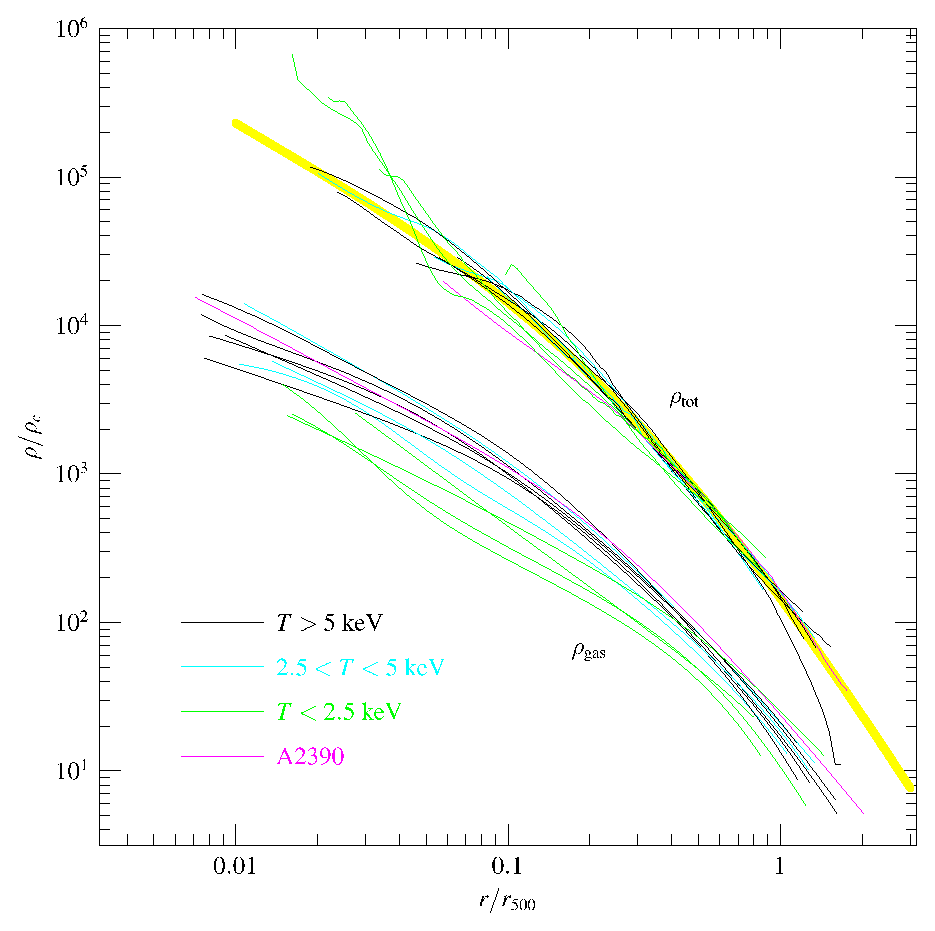
\includegraphics[width=0.6\linewidth]{chapter8/rhoprof.eps}}
	\subfigure[Temperature profiles.]
	{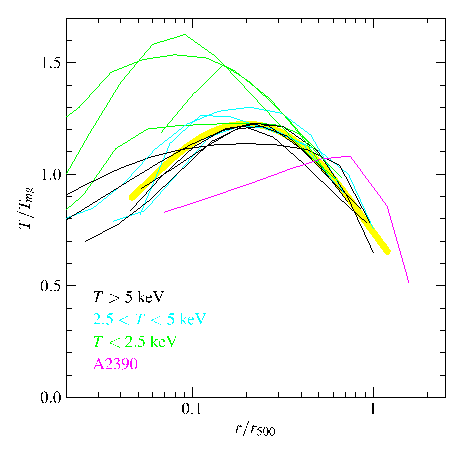
\includegraphics[width=0.6\linewidth]{chapter8/Tprof.eps}}
	\caption{Scaled density and temperature profiles for galaxy clusters
	observed with CHANDRA by \citep{Vikhlinin2006}. The yellow line are a NFW
	fit to the total gas density and a average fit to the temperature profiles.}
	\label{fig:profiles}
\end{figure}
It is apparent, that the NFW profile provides a good fit for the density
profile of the total mass of the clusters. The scatter in the baryonic density 
profiles is significantely larger and for lower temperature clusters the
profiles are flatter towards the center of the cluster. The temperature
profiles also show signs of self-similarity, at least for the higher
temperature clusters $T > \unit[2.5]{keV}$, which are fitted by
\begin{align}
\frac{T(r)}{T_{mg}} = 1.35 \frac{(x/0.045)^{1.9} + 0.45}{(x/0.045)^{1.9}+1}
\frac{1}{\lrb{1+(x/0.6)^2}} 
\end{align}
where $x=r/r_{500}$ according to \citep{Vikhlinin2006}. Also visible from the
temperature fit are a isothermal plateau at $r \approx \unit[0.2]{r_{500}}$ and
the significant decrease of temperature towards the center. This behavior is
often
explained by assuming some cooling mechanism. Theoretically cooling
should lead to lower pressure in the center of the cluster, thereby leading to
an even denser core to maintain hydrostatic equilibrium. But, because cooling is
even more effective at lower densities, this process is instable leading to
catastrophic cooling of the core, which is not observed, giving rise to the
so-called ``cluster cooling flow problem''. Observationally emissions from the
central cluster gas can be detected for gas temperatures between the ambient
temperature $T_0$ and $\sim T_0/2$, but not below $<T_0/3$ \citep{Peterson2003},
so some sort of heating mechanism seems to be inhibiting the cooling below this 
temperature. There are plenty of candidates for this - supernovae, outflows
from active galactic nuclei, thermal conduction and turbulent mixing - but
there is still no consensus on the relative importance of these mechanisms.
Turbulence is especially interesting because it was also
suggested by \citet{Nagai2007} as mechanism, which might explain some
deviations in the computation of the total mass,
based on the assumption of hydrostatic equilibrium, without taking
turbulent pressure into account. 

\subsection{Turbulence in the ICM}
The ``bottom-up'' model or hierarchical model of cosmological structure
formation
\citep[eg.,][]{Ostriker1993} explains the build up of clusters through a
sequence of mergers of lower-mass systems (stars $\rightarrow$ galaxies
$\rightarrow$ groups $\rightarrow$ clusters). In particular, mergers of galaxies
play a fundamental role in 
determining the structure and dynamics of massive clusters of galaxies. It is
found that major mergers induce temperature inhomogeneities and bulk motions
with velocities $> \unit[1000]{km\ s^{-1}}$ in the intracluster medium (ICM)
\citep{Norman1999a}. This results in complex hydrodynamic flows where most of
the kinetic energy is quickly dissipated to heat by shocks, but some part may in
principle also excite long-lasting turbulent gas motions.

In numerical simulations of merging clusters \citep{Schindler1993, 
Roettiger1997,Ricker2001,Takizawa2005} it has been shown that infalling
subclusters generate a laminar bulk flow, but inject turbulent motions via
Kelvin-Helmholtz instabilities at the interfaces between the bulk flows and the
primary cluster gas. Such eddies redistribute the energy of the merger through
the cluster volume and decay with time into more and more random and turbulent
velocity fields, eventually developing a turbulent cascade with a spectrum of
fluctuations expected to be close to a Kolmogorov spectrum \citep{Dolag2005}. 

The turbulent nature of the flow could be directly confirmed with the help of
high-resolution X-ray spectroscopy of emission line broadening of lines of
heavy ions. It has been suggested \citep{Sunyaev2003}, that the X-ray
microcalorimeters (XRS) on board of the X-ray satellite ASTRO-E2\footnote{Also
called \emph{Suzaku}.} should be able to detect this broadening. But due to a
critical flaw discovered in the XRS instrument in August 2005, this test has to
be
postponed until future instruments like XEUS are available. Nevertheless other
observations have revealed some signature for turbulence in the ICM.
For example \citet{Schuecker2004} analyzed the pressure
fluctuation spectrum of the Coma cluster claiming that it scales according to
Kolmogorov-Obukhov theory (see figure \ref{fig:schuecker}).

\begin{figure}[tp]
\centering
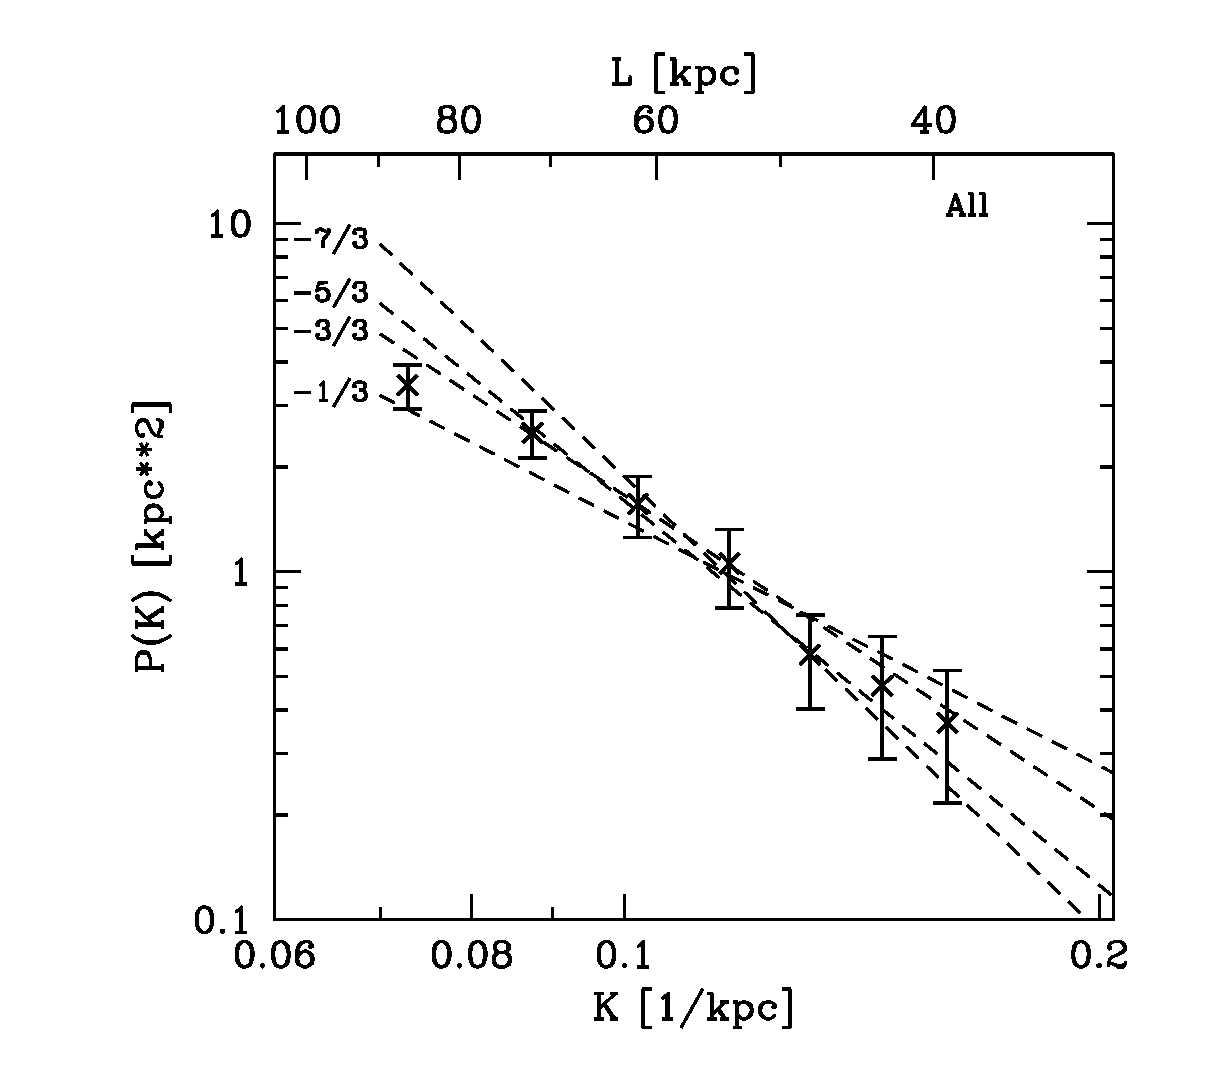
\includegraphics[width=0.7\linewidth]{chapter8/1039fg12.eps}
\caption{Observed projected shot-noise-subtracted 
power spectral densities (dots with $1\sigma$ error bars) compared with model
predictions (dashed lines). From \citet{Schuecker2004}.}
\label{fig:schuecker}
\end{figure}
\begin{figure}[tp]
\centering
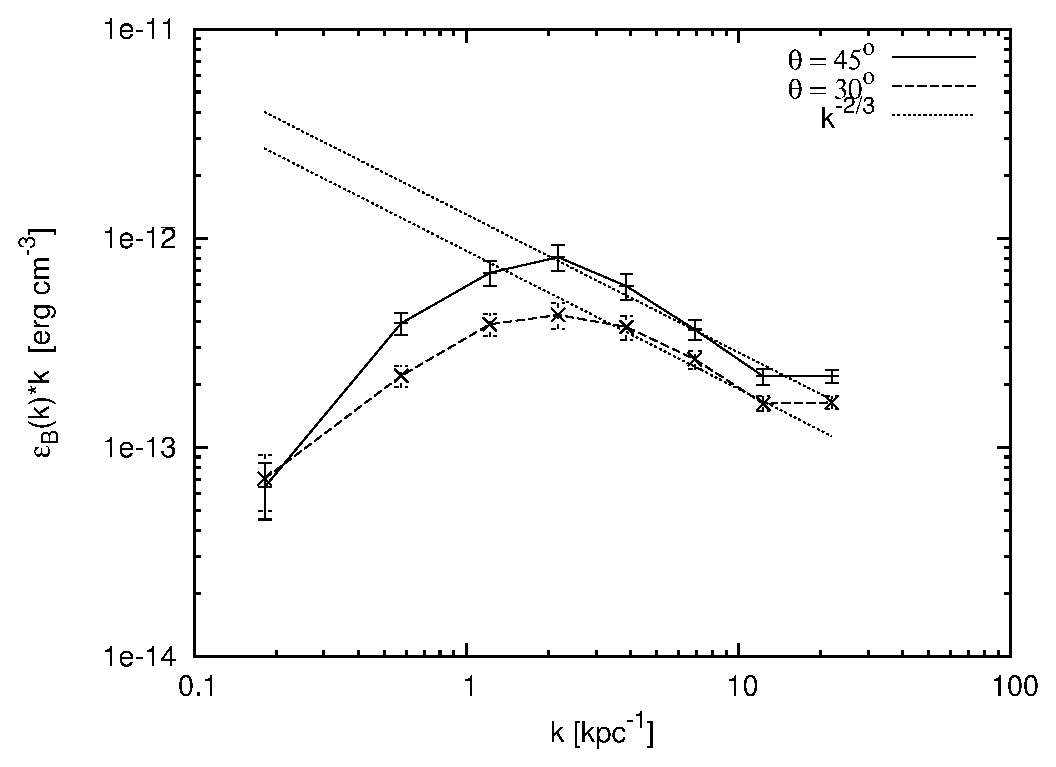
\includegraphics[width=0.7\linewidth]{chapter8/fig7.eps}
\caption{Power spectra for two different
inclination angles $\theta = 30^\circ$ and $\theta = 45^\circ$.
For comparison a Kolmogorov-like power spectrum is
plotted as a straight dashed line. One can see that the calculated
power spectra follow such a power spectrum over at least one order of
magnitude. From \citet{Vogt2005}.}
\label{fig:vogt}
\end{figure}

\citet{Vogt2005} makes
use of the Faraday rotation effect to investigate the magnetic field structure
of the ICM in the Hydra cluster. They extract magnetic field strength power
spectra from their data and find a Kolmogorov scaling behavior below a
length scale of \unit[1]{kpc} (see figure \ref{fig:vogt}) . 

Furthermore the broadening of the iron abundance profile
in the core of the Perseus cluster \citep{Rebusco2005} and other galaxy
clusters \citep{Rebusco2006} and the lack of 
resonant scattering in the $\unit[6.7]{keV}$ He-like iron K$_{\alpha}$ line in
the Perseus cluster \citep{Churazov2004} can also be interpreted as evidence for
the turbulent state of the ICM. 


 

 

\chapter{Simulations of galaxy clusters}\label{clustersim}
\section{Details of the simulations}
We performed two simulations of cluster formation with Enzo following
\citet{Iapichino2008}. One simulation was done with the Schmidt SGS model
including the Sarkar corrections and some additional modifications described
below. For comparsion we conducted a second simulation without SGS model. In the
following section we describe the common features of these two simulations, in
section \ref{numissues} we describe some additional numerical issues, which had
to be taken into account when doing a cluster simulation with SGS model in
comoving coordinates. 
\subsection{Common features}\label{common}
The simulations were done using a flat (critical density $\Omega=1$) cold dark
matter (CDM) background cosmology with a dark energy density
$\Omega_{\Lambda}=0.7$, a total (including baryonic and dark matter) matter
density $\Omega_{m}=0.3$, a baryonic matter density $\Omega_{b}=0.04$, the
Hubble parameter set to $h=0.7$, a galaxy fluctuation amplitude $\sigma_8=0.9$,
and a scalar spectral index $n=1$. Both simulations were started with the same
initial conditions at redshift $z_{ini}=60$, using the \citet{Eisenstein1999}
transfer function, and evolved to $z=0$. The simulations were adiabatic with a
heat capacity ratio $\gamma=5/3$ assuming a fully ionized gas with a mean
molecular weight $m_{\mu}= \unit[0.6]{u}$. Cooling physics, magnetic fields,
feedback, and transport processes are neglected. 

The simulation box had a comoving size of $\unit[128]{Mpc\ h^{-1}}$. It was
resolved with a root grid (level $l=0$) of $128^3$ cells and $128^3$ N-body
particles. A static child grid ($l=1$) was nested inside the root grid with a
size of 
64 Mpc/h, $128^3$ cells and $128^3$ N-body particles. The mass of each particle
in this grid was $\unit[9 \times 10^9]{M_{\odot}\ h^{-1}}$. Inside this grid, in
a volume of $\unit[38.4]{Mpc\ h^{-1}}$, adaptive grid refinement from level
$l=2$ to $l=6$ was enabled using a overdensity refinement criteria as described
in \citet{Iapichino2008} with an overdensity factor $f=4.0$. The refinement
factor between two levels was set to $r=2$, allowing for a effective resolution
of $8196^3$ cells or $\unit[15.6]{kpc\ h^{-1}}$.

The static and dynamically refined grids were nested around the place of
formation of a galaxy cluster, identified by \citet{Iapichino2008} using the
HOP algorithm \citep{Eisenstein1998}. The cluster had a virial mass of
$M_{vir}=\unit[5.49 \times 10^{14}]{M_{\odot}\ h^{-1}}$ and a virial radius of
$R_{vir}=\unit[1.33]{Mpc\ h^{-1}}$ for both simulations.  

\subsection{Numerical issues}\label{numissues}
Running robust simulations including a SGS model like the Schmidt or Sarkar
model in a comoving cosmological background requires some additional techniques
not yet discussed. Apart from the additional terms due 
to comoving coordinates in the filtered equations, these techniques help to
handle the extreme high turbulent Mach numbers, which appear on the coarsest
grids in these simulations and are briefly described in the following sections.

\subsubsection{Filtered equations of fluid dynamics in comoving coordinates}
Filtering the equations of fluid dynamics in comoving coordinates
\eqref{eq:commass2}-\eqref{eq:cometot2} can be done in the same way as
filtering the equations in cartesian coordinates as shown in chapter \ref{FE}.
As a result we get
\begin{align}
\pd{t}\fil{\tilde{\rho}} + \fa\pd{x_j}\hat{u}_j \fil{\tilde{\rho}} =& 0,
\label{eq:filcommass2}\\
\begin{split}
\pd{t}\fil{\tilde{\rho}} \hat{u}_i 
+ \fa\pd{x_j}\hat{u}_j \fil{\tilde{\rho}} \hat{u}_i =& 
-\fa\pd{x_i}\fil{\tilde{p}}+ \fa\pd{x_j}\fil{\sigma'_{ij}} 
+\fil{\tilde{\rho}}\hat{g}^*_i 
-\fa\pd{x_j}\hat{\tau}(u_i,u_j)\\
&- \fh \fil{\tilde{\rho}} \hat{u}_i,
\label{eq:filcommom2}
\end{split}
\\
\begin{split}
\pd{t}\fil{\tilde{\rho}}e_{res}+\fa\pd{x_j}\hat{u}_j\fil{\tilde{\rho}}e_{res}=&
-\fa\pd{x_i}\hat{u}_i\fil{\tilde{p}}
+\fa\pd{x_j}\hat{u}_i\fil{\sigma'_{ij}}
+\fa\fil{\tilde{\rho}}\hat{u}_i\hat{g}^*_i\\
&-\fh(\fil{\tilde{\rho}}e_{res}
+\frac{1}{3}\fil{\tilde{\rho}}\hat{u}_i\hat{u}_i+\fil {\tilde{p}})\\
&+\fil{\tilde{\rho}}(\lambda+\epsilon)
-\fa\hat{u}_i\pd{x_j}\hat{\tau}(u_i,u_j)
-\fa\pd{x_j}\hat{\tau}(u_j,e_{int}),\label{eq:filcomresetot}
\end{split}
\\
\pd{t}\fil{\tilde{\rho}}e_t+\fa\pd{x_j}\hat{u}_j\fil{\tilde{\rho}}e_t=&
\mathbb{D} +\Gamma
-\fil{\tilde{\rho}}(\lambda+\epsilon)
-\fa\hat{\tau}(u_j,u_i)\pd{x_j}\hat{u_i}
-2\fh\fil {\tilde{\rho}}e_t.
\label{eq:filcomet}
\end{align}

In the source code of Enzo the derivatives are always taken with respect
to $r_i=a x_i$ and the additional terms due to comoving coordinates in 
momentum and resolved energy equation are already implemented. So the only term
we had to implement additionally compared to the non-comoving case was the term
$2\fh\fil {\tilde{\rho}}e_t$ in the equation of turbulent energy. Furthermore
for the subgrid model terms it is necessary to take into account that
the Jacobian of the velocity in comoving coordinates is\footnote{See equation
\eqref{eq:cotrans5} in the Appendix.}
\begin{align}
J_{ij} = \pd{r_i}v_j&=\fa\pd{x_i}u_j + \fh\delta_{ij}.
\end{align}
The tracefree rate of strain tensor in comoving coordinates for example can then
be easily expressed in terms of the Jacobian of the velocity field
\begin{align}
S^*_{ij}=\frac{1}{2}\lra{J_{ij}+J_{ji}}-\frac{1}{3}\delta_{ij}J_{kk}.
\end{align}
Basically all terms in the subgrid model using derivatives of the resolved
velocity are therefore written in terms of the Jacobian of the velocity.

\subsubsection{Turbulent energy cutoff and lower limit for temperature}
High turbulent Mach numbers occur in cosmological simulations especially in the
very cold, low-density voids of the computational domain. To make sure that in
our adiabatic simulation the temperature and therefore the sound speed doesn't
drop to unphysical low values we introduced a lower limit of the temperature
$T_{min}=\unit[10]{K}$. This value is reasonable, since no gas in the
universe can have a temperature lower than the cosmic microwave background
temperature of 2.7 K for a longer time. Since there are presumably more
heating mechanisms like UV-heating, choosing 10 K as a lower limit seems to be
a rational choice. 

On the other side, low density gas can be accelerated very quickly in a
gravitating field, leading to high velocity gradients, which lead to 
production of high amounts of turbulent energy according to the turbulent
viscosity hypothesis. However the validity of the turbulent viscosity
hypothesis has never been tested or verified in astrophysical
flows. We are therefore free to assume that for flows with high velocity
gradients, the production of turbulent energy is restricted and use as an
upper limit of the turbulent Mach number $M_{t,max}=\sqrt{2}$. The exact value
of this limit is based on the idea that in an isothermal gas (speed of sound 
$c_{\text{s,iso}} = \frac{p_{th}}{\rho}$), the total pressure can be expressed as
\begin{align}
p_{tot}=\rho c_{\text{s,iso}}^2 + \frac{1}{3}\rho q^2 = \gamma_{\text{eff}} \rho c_{\text{s,iso}}^2.
\end{align}
If we assume that $\gamma_{\text{eff}}$ is not allowed to be higher than the
adiabatic value $\gamma=5/3$, we have to limit the isothermal turbulent Mach number to
$\frac{q}{c_{\text{s,iso}}} \leq \sqrt{2}$.  

\subsubsection{Treatment of shocks}
Shocks form unavoidably during cosmological structure formation due to
infalling plasma which accretes onto filaments, sheets, and halos, as well as
due to supersonic flows associated with merging substructures
\citep{Pfrommer2006}. But shocks are the most localized and anisotropic
features of a flow and therefore cannot be treated by an SGS model, which 
is based on the assumption of isotropy of the flow on the subgrid
scales.\footnote{Also see chapter \ref{amrles}.} So in principle, shocks should
be treated by the mechanisms of AMR alone and the SGS model should
not influence the shocks. That's why we implemented a simple shock detector
\begin{align}
-\ppd{r_i}{v_i} l_{\Delta} > c_s,
\end{align}
which marks all cells, where the velocity increments are greater than the
speed of sound, as shocks. At these cells, we disable the SGS model, which
means no production or dissipation of turbulence takes place. The turbulent
energy is only advected in these cells.   

\section{Results}
\subsection{Energy conservation}
Energy conservation is crucial for any adiabatic fluid dynamic simulation.
However it is difficult to test for this directly in our setup, since we cannot
extract easily the energy injected by gravity into the system. By plotting the
time development of the mass weighted mean total energy in the system, which is
for the simulation without SGS model the sum of mass weighted mean internal
energy and mass weighted mean kinetic energy and for the simulation with Sarkar
model the sum of mass weighted means of internal, kinetic and turbulent energy,
we can still gain some insights into the differences between the two
simulations. 

\begin{figure}[tp]
\centering
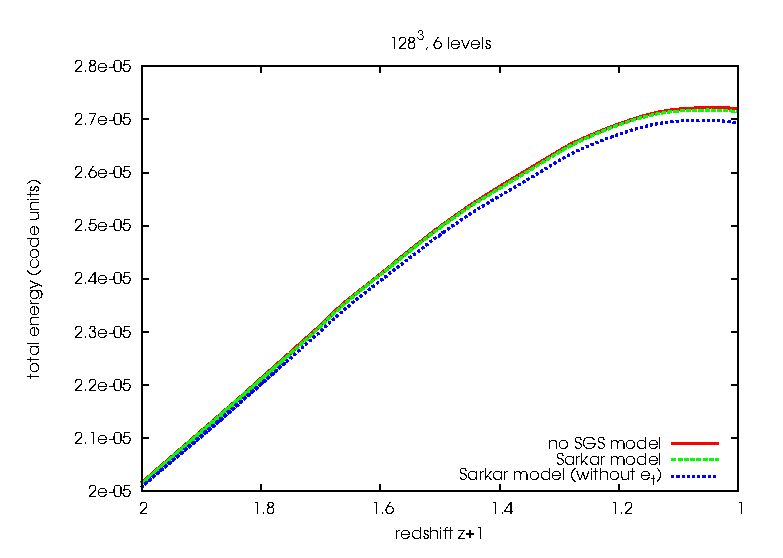
\includegraphics[width=0.7\linewidth]{chapter9/energyerror.eps}
\caption{Time development of total energy in cluster simulation with and
without SGS model.}
\label{fig:etot}
\end{figure}

This is what has been done in figure \ref{fig:etot}. From it we can see
that the time development of the total energy is nearly identical, if we take
the turbulent energy into account when computing the total energy of the
simulation with Sarkar model. On the other side, the difference between the sum
of kinetic and internal energy between the simulations seems to be again mostly
accounted for by the turbulent energy, a result similar to what was already
found in the simulations of driven turbulence.\footnote{See section
\ref{numenergy}.}
We can also infer from figure \ref{fig:etot}, that the SGS model mainly changes
the ratio of mean internal to mean kinetic energy and does not have much
influence on the mean potential energy of the system. However, this is to be
expected, since most of the gravitational potential is due to dark matter
anyway, and we do not model the influence of gravity on subgrid scales and vice
versa in our SGS model. This leads us to conclude that the general effects of
our SGS model in a selfgravitating fluid are very similar to the effects found
in the driven turbulence simulations without self gravity.  

\subsection{Mass fractions of different gas phases}
The IGM on large scales of the universe can be classified roughly into four
phases according to gas temperature: the hot gas with $T > \unit[10^7]{K}$
inside and around clusters; the warm-hot intergalactic medium (WHIM) with
$\unit[10^5]{K} < T < \unit[10^7]{K}$ found mostly in filaments; the low
temperature WHIM with $\unit[10^4]{K} < T < \unit[10^5]{K}$ distributed mostly
as sheetlike structures; and the diffuse cold gas with $T < \unit[10^4]{K}$
residing mostly in voids \citep{Cen1999,Kang2005}. To investigate the influence
of the SGS model on these different gas phases, we plotted the time development
of the mass fractions according to each of the phase for the simulation with
and without SGS model (figure \ref{fig:massfrac1a} and \ref{fig:massfrac1b}).
\begin{figure}[tp]
\centering
\subfigure[No SGS model.]{
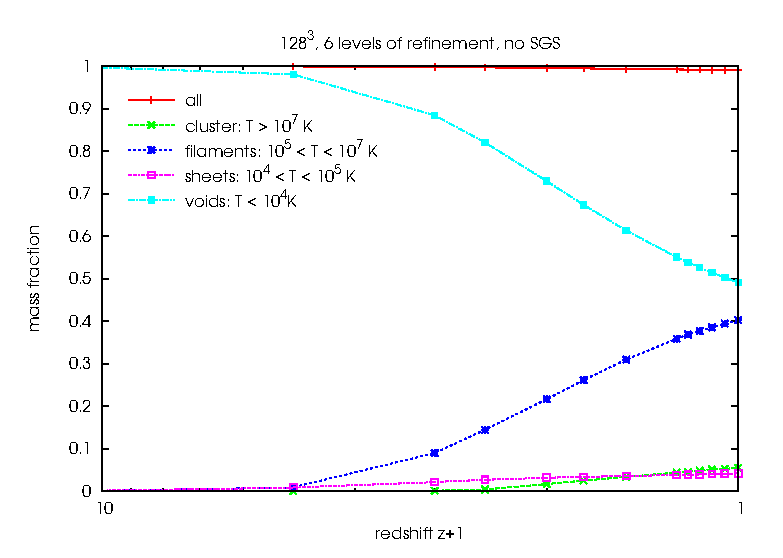
\includegraphics[width=0.45\linewidth]{chapter9/mass_red_nosgs.eps}
\label{fig:massfrac1a}}
\subfigure[SGS model.]{
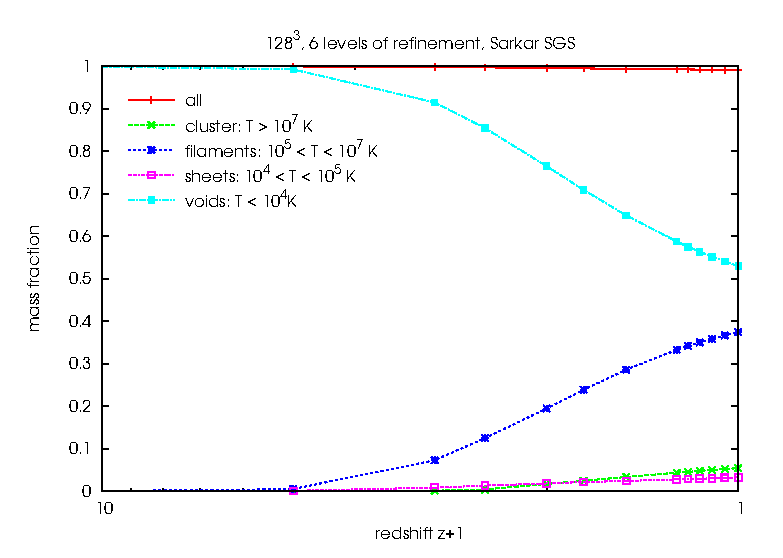
\includegraphics[width=0.45\linewidth]{chapter9/mass_red_sar.eps}
\label{fig:massfrac1b}}
\caption{Time development of mass fractions of different gas phases in the
whole simulation box had with a comoving size of
$\unit[128]{Mpc\ h^{-1}}$.}
\end{figure}
We also show the mass fractions of each gas phase at redshift $z=0$ in table
\ref{tab:massfrac1}. 
\begin{table}[htbp]
\begin{center}
\begin{tabular}{lcccc}
\hline
Run & 
$\frac{m_{\text{cluster}}}{m_{\text{all}}}\ [\%]$ &
$\frac{m_{\text{filaments}}}{m_{\text{all}}}\ [\%]$ &
$\frac{m_{\text{sheets}}}{m_{\text{all}}}\ [\%]$ & 
$\frac{m_{\text{voids}}}{m_{all}}\ [\%]$ \vspace*{1mm} \\
\hline
\hline
no SGS & 5.50 & 40.3 & 4.22 & 49.1\\ 
SGS & 5.47 & 37.5 & 3.28 & 53.0 \\
\hline
\end{tabular}
\end{center}
\caption{Mass fractions of different gas phases at redshift $z=0$.}
\label{tab:massfrac1}
\end{table}
The results seem to indicate that the SGS model leads to higher mass fraction
of the voids and a lower mass fraction of the filaments compared to the
simulation without SGS model. However our simulation domain is not very well
resolved outside the central region, since we do not allow for adaptive
refinement there. If we restrict our analysis to the adaptively refined region
in the box with a size of $\unit[38.4]{Mpc\ h^{-1}}$, the differences between
the simulation with SGS model and without SGS model vanish 
(figure \ref{fig:massfrac2a} and \ref{fig:massfrac2b}).
\begin{figure}[tp]
\centering
\subfigure[No SGS model.]{
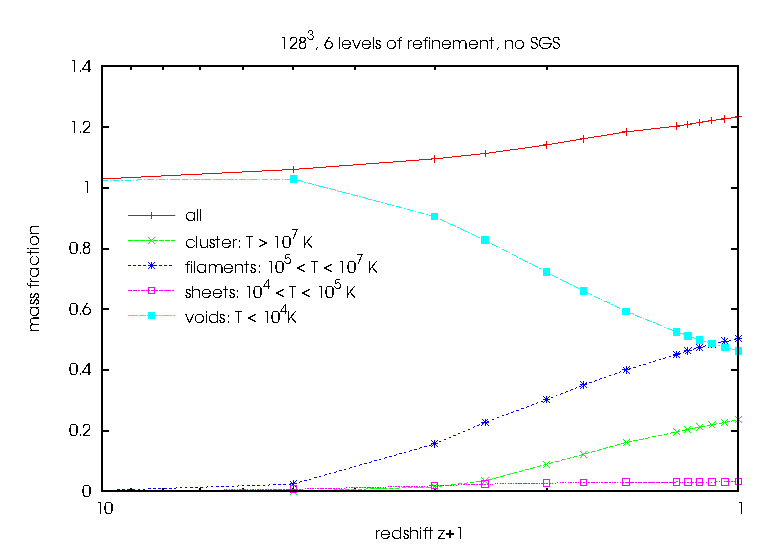
\includegraphics[width=0.45\linewidth]{chapter9/mass_red_nosgs_small.eps}
\label{fig:massfrac2a}}
\subfigure[SGS model.]{
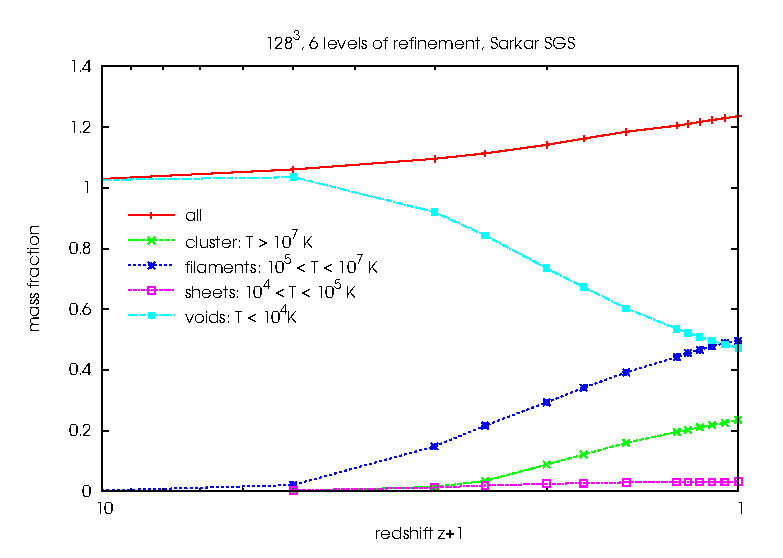
\includegraphics[width=0.45\linewidth]{chapter9/mass_red_sar_small.eps}
\label{fig:massfrac2b}}
\caption{Time development of mass fractions of different gas phases in the
centered subset of the simulation box with a comoving size of 
$\unit[38.4]{Mpc\ h^{-1}}$. One can see that the total mass in this open region
is not conserved.}
\end{figure}
This can also be seen from the mass fractions at redshift $z=0$ normalized to
the total mass in the central region in table \ref{tab:massfrac2}. 
\begin{table}[htbp]
\begin{center}
\begin{tabular}{lcccc}
\hline
Run & 
$\frac{m_{\text{cluster}}}{m_{\text{all}}}\ [\%]$ &
$\frac{m_{\text{filaments}}}{m_{\text{all}}}\ [\%]$ &
$\frac{m_{\text{sheets}}}{m_{\text{all}}}\ [\%]$ & 
$\frac{m_{\text{voids}}}{m_{all}}\ [\%]$ \vspace*{1mm} \\
\hline
\hline
no SGS & 19.2 & 40.8 & 2.61 & 37.5\\ 
SGS & 19.0 & 40.1 & 2.64 & 38.2 \\
\hline
\end{tabular}
\end{center}
\caption{Mass fractions of different gas phases at redshift $z=0$ for the
adaptively refined region with a size of $\unit[38.4]{Mpc\ h^{-1}}$.}
\label{tab:massfrac2}
\end{table}
From these results we conclude that the SGS model has no or only very little
influence on the mass fractions of the different gas phases in the simulations.
For the important mass fraction of the WHIM we get $ \approx 38\%$, which is 
higher than found by \citet[simulation B1]{Dave2001} ($ \approx 32\%$) with a
lower resolution AMR simulation, but lower than found by \citet{Gottlober2006}
($ \approx 40\%$), who used smoothed particle hydrodynamic (SPH) with 
$2 \times 1024^3$ particles to simulate a box of size $\unit[500]{Mpc\ h^{-1}}$;
so we are also consistent with the literature in this respect.

\subsection{Development of turbulence in different gas phases}
The eddy turnover time $t_l$ associated with a scale $l$ 
\begin{align}
t(l) = \frac{l}{q(l)}
\end{align}
is the typical time for a structure of size $\sim l$ to undergo a significant
distortion due to turbulent motions characterized by the
typical turbulent velocity $q(l)$ at that scale \citep{Frisch1995}. So if we
divide the age of the universe $t(z)$ by the eddy turnover time, we get the
number of eddy turnovers 
\begin{align}
n(l,z)=\frac{t(z)}{t(l)}
\end{align}
at a given redshift $z$ at a scale $l$. If $n > 1$, there has been enough time 
for eddies of size $l$ to cascade down to smaller scales and we can call the
fluid turbulent at scale $l$. 

In static grid simulations one often chooses to use the grid resolution
$l_{\Delta}$ as characteristic length scale and to compute a characteristic
velocity and eddy turnover time for this scale. However in an AMR code it is not
trivial to compute the turbulent velocity $q_l$ associated with a characteristic
length scale $l = l_{\Delta}$, since $l_{\Delta}$ is varying in time and space.
To circumvent this difficulty, we assume that below the grid resolution at a
certain position turbulent velocity scales according to Kolmogorov
\begin{align}
q(l) \sim l^{1/3}.
\end{align}
We thereby assume that locally, the cascade starts at a different length scale
characterized by the different resolution of our grid at that position. We also
assume that our refinement criterion tracks and finds the regions inside the
fluid, which do not scale according to Kolmogorov, and refines them until a
Kolmogorov scaling is reached. Of course one might doubt that our refinement
criterion based on overdensity will accomplish that. But since in cosmological
simulations gravity is basically the energy-injecting force in the fluid and
gravity is strongest in regions of high density, one can argue that in regions
of high density, the Kolmogorov cascade starts at smaller length scales and
the energy injecting scales in these regions have to be refined with a finer
grid. Of course a criterion solely based on density might be necessary,
but is not at all sufficient to track regions of Non-Kolmogorov scaling.
More research needs to be done in this direction, but it is outside of the 
scope of this work. 

For the analysis in our work, we adopt the hypothesis of local Kolmogorov
scaling below the grid resolution. As a characteristic scale of our analysis,
we choose the length scale of our highest resolved regions, which is 
$l_{min}=\unit[15.6]{kpc\ h^{-1}}$. The turbulent velocity in the highest
resolved regions can be directly computed from the values of the turbulent
energy $q(l) = \sqrt {2 e_t}$ on the grid; the turbulent velocity in less
refined regions is scaled down according to our local Kolmogorov hypothesis as
\begin{align}
q(l_{min}) = q(l_{\Delta}) \lra{\frac{l_{min}}{l_ {\Delta}}}^{1/3}
\label{eq:vturbscaled}.
\end{align}
Using this scaled turbulent velocity to compute the eddy turnover time, we 
plotted the mean mass weighted number of eddy turnovers at $l_{min}$ with
respect to redshift (see figure \ref{fig:eddy}). 
\begin{figure}[tp]
\centering
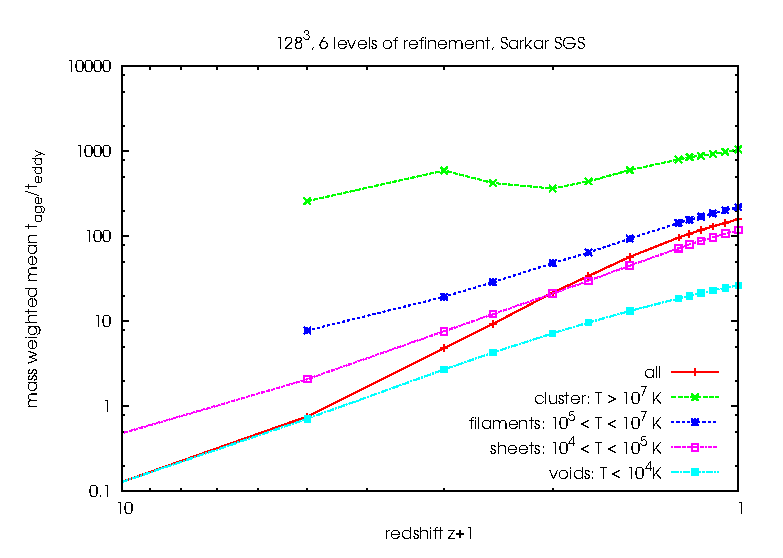
\includegraphics[width=0.7\linewidth]{chapter9/eddy_red_sar.eps}
\caption{Mean number of eddy turnovers for gas phases of
different temperature over time.}
\label{fig:eddy}
\end{figure}
We can clearly see from this graph, that starting from a redshift $z=2$ all gas
phases are turbulent at the scale $l_{min}=\unit[15.6]{kpc\ h^{-1}}$. We also
see that the amount of turbulence in terms of eddy turnover times is higher in
regions of higher temperature and therefore highest in the cluster gas.    

Another important measure for turbulence is the turbulent Mach number
introduced in section \ref{dimanalsgs}. Like the eddy turnover time, the
turbulent Mach number is scale dependent
\begin{align}
M_t(l)=\frac{q(l)}{c_s}.
\end{align}
In figure \ref{fig:machturb} we plot the mean mass weighted turbulent Mach
number characteristic for the scale of our analysis 
$l_{min}=\unit[15.6]{kpc\ h^{-1}}$ making again use of our local Kolmogorov
hypothesis.
\begin{figure}[tp]
\centering
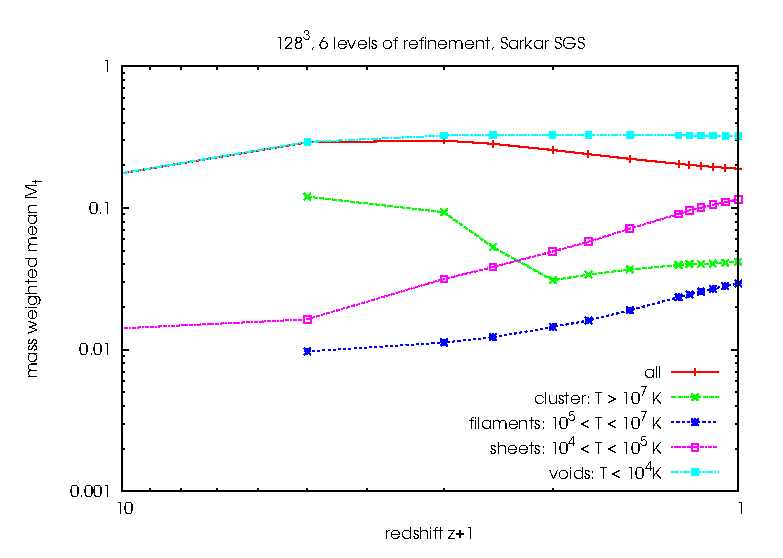
\includegraphics[width=0.7\linewidth]{chapter9/machturb_red_sar.eps}
\caption{Mean turbulent Mach number at a scale 
$l_{min}=\unit[15.6]{kpc\ h^{-1}}$ for gas phases of different temperature over
time.}
\label{fig:machturb}
\end{figure}
It is evident that the turbulence at $l_{min}$ is subsonic in all gas phases
during the whole time of the simulation. At redshift $z=0$ the average
turbulent Mach number is $\approx 0.2$. If the
amount of turbulence would be equal in each gas phase one would expect the
turbulent Mach number to scale $\sim 1/c_s \sim 1/\sqrt{T}$. However this is
not the case. The cluster gas is much more turbulent than estimated by this
simple scaling relation; in fact there is more turbulent energy compared to 
internal energy in the hottest gas phase than in the WHIM, although there is a
substantial drop of the turbulent Mach number between redshift $z=1-2$. The
drop in turbulent Mach number is presumably due to heating of the cluster gas
during a phase of major mergers at that time. In the next section, we will 
present some further evidence for this interpretation.  

\subsection{Scaling of turbulent energy}
In chapter \ref{numtest} we studied the scaling of the turbulent energy
with the resolution and were able to show that the scaling
of turbulent energy in our simulations of driven turbulence actually follows
the Kolmogorov scaling law. In this section we repeat this analysis for our 
cluster simulation. Figure \ref{fig:tuerescluster} shows the time development of
the mass weighted mean turbulent energy for every level of our AMR simulation. 
\begin{figure}[tp]
\centering
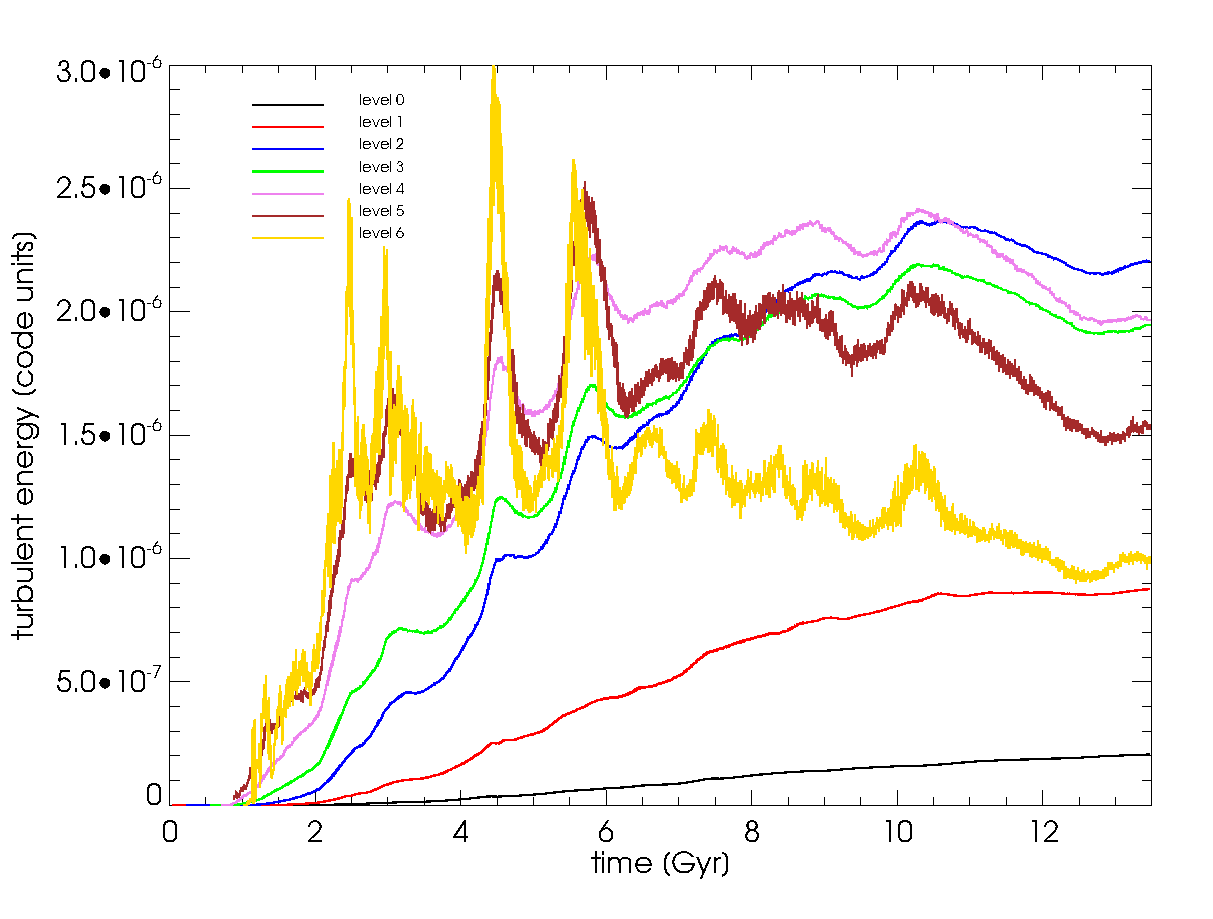
\includegraphics[width=0.7\linewidth]{chapter9/tuemwrescluster128sar.eps}
\caption{Time development of mean turbulent energy over time for each level of
refinement.}
\label{fig:tuerescluster}
\end{figure}
We see from the plot, that the turbulent energy on the higher levels (meaning
at smaller scales) is higher at times $t<\unit[6]{Gyr}$. Later this picture
changes, but not completely. For example the turbulent energy on level 4 stays
above the turbulent energy of level 3 for the whole simulation time. Also
striking are the high fluctuations in the time $\unit[2]{Gyr}<t<\unit[6]{Gyr}$,
which correspond to a redshift $z=3-1$ of the turbulent energy at the smaller
scales. This is also the time when the turbulent Mach number inside the
cluster drops significantly (see last section), so we can interpret these high
fluctuations as further evidence for violent major mergers, that happen at that
time, producing turbulent energy, which is then dissipated into internal energy
heating up the cluster gas. However at the time $t>\unit[13]{Gyr}$, the
simulation seems to reach some kind of stable state, similar to what is found in
driven turbulence simulations. We therefore can compute mean turbulent energies
by averaging the turbulent energy from $t=\unit[13]{Gyr}$ to the end of the
simulation and plot them against the grid length scale of the associated level.
The result (in terms of the turbulent velocity) can be seen in figure 
\ref{fig:tuefitcluster}. 
\begin{figure}[tp]
\centering
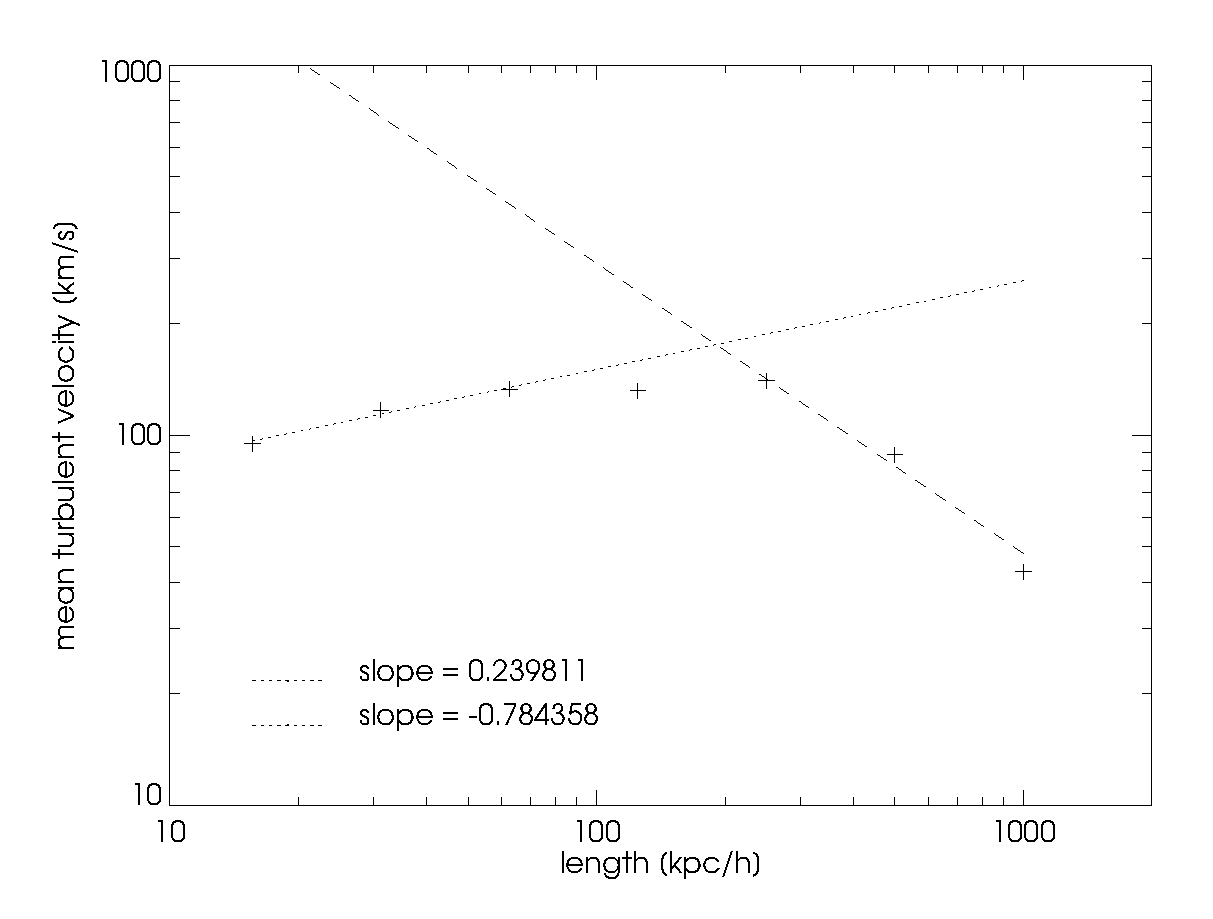
\includegraphics[width=0.7\linewidth]{chapter9/tuemwfitcluster128.eps}
\caption{Scaling of mean turbulent energy. The dotted line is a fit showing the
scaling behavior of turbulent energy below $\unit[100]{kpc\ h^{-1}}$, the dashed
line is a fit showing the scaling behavior above $\unit[100]{kpc\ h^{-1}}$.}
\label{fig:tuefitcluster}
\end{figure}
It is obvious that this is no Kolmogorov scaling. However, we do not expect to
see a Kolmogorov scaling again, since, as explained in the last section, we
assume the resolved regions to be non-Kolmogorov anyway. Still the result is
interesting, showing a peak in the turbulence around $\unit[100]{kpc\ h^{-1}}$
and a drop off towards higher and smaller scales. Also shown in the figure are
power-law fits, which gave a scaling of $q \sim l^{-0.78}$ for scales bigger
than $\unit[100]{kpc\ h^{-1}}$ and a scaling of $q \sim l^{0.24} \sim l^{1/4}$
for smaller scales. If one wants to interpret this result in terms of a
turbulent cascade, one could say that up to a length scale of  
$\unit[100]{kpc\ h^{-1}}$, energy is injected into the system, cascading down
towards smaller scales with a scaling behavior $q \sim l^{1/4}$ flatter than
expected for a Kolmogorov scaling with $q \sim l^{1/3}$. But, assuming our local
Kolmogorov hypothesis holds, it would follow, that below the grid resolution
of $\unit[15.7]{kpc\ h^{-1}}$ the cascade should be Kolmogorov again. Of course
a interpretation like this is highly speculative; much more data on
turbulence in cluster simulations is necessary to show that the
observed power-law scalings are real indeed.

\subsection{Radial profiles of the cluster}
As mentioned in section \ref{common}, the simulation is centered around a
galaxy cluster with a virial mass of $M_{vir}=\unit[5.49 \times
10^{14}]{M_{\odot}\ h^{-1}}$ and a virial radius of $R_{vir}=\unit[1.33]{Mpc\
h^{-1}}$ for both simulations, which center is identified using the
HOP algorithm. In the following we present plots of radial profiles of several
quantities around the center of this cluster (figure
\ref{fig:dens}-\ref{fig:vturb})
obtained by using a modified version\footnote{We modified \texttt{enzo\_anyl} to
allow plotting of SGS model quantities like the turbulent velocity.} of the
\texttt{enzo\_anyl} tool, which is part of the public Enzo release.   
\begin{figure}[tp]
\centering
\subfigure[Gas density.]{
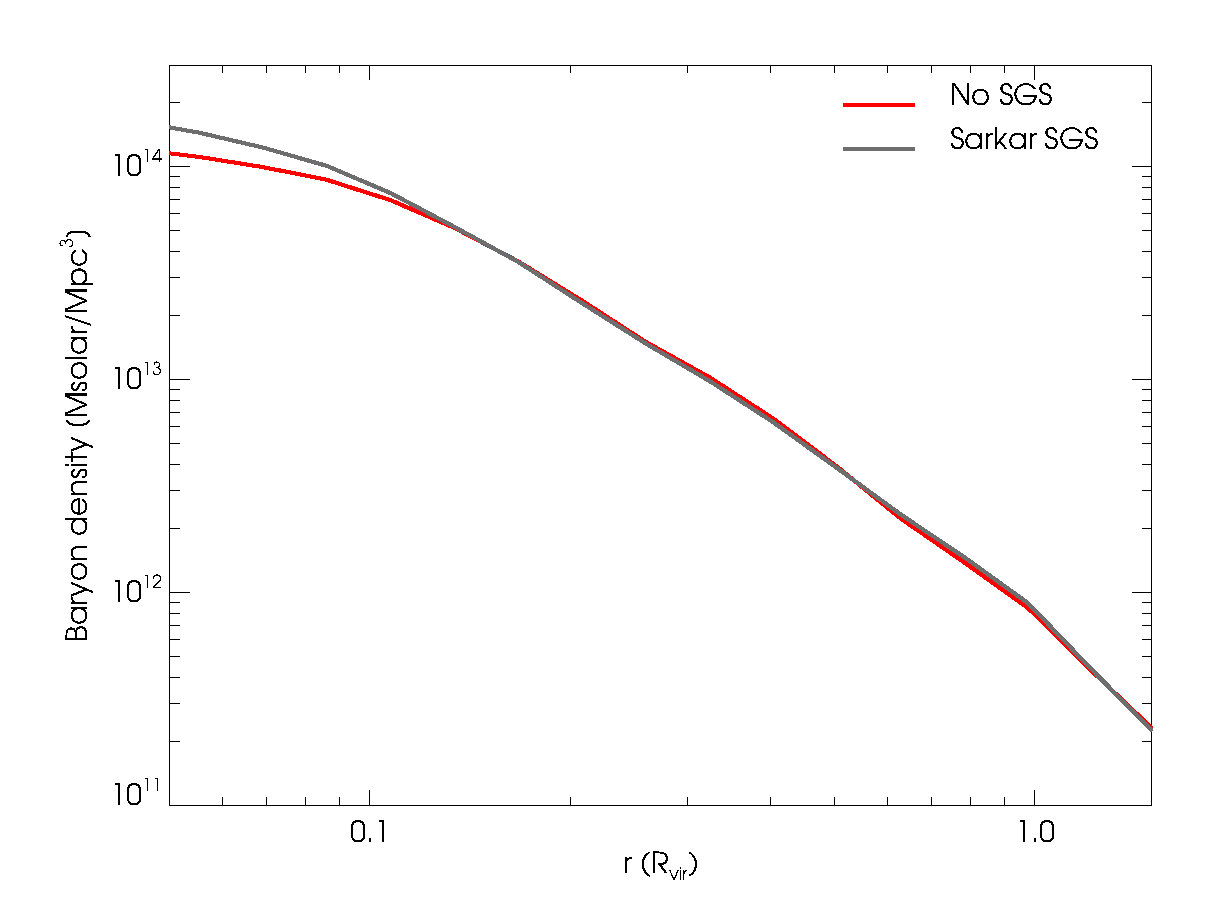
\includegraphics[width=0.45\linewidth]{chapter9/d_gaslog.eps}
\label{fig:dens}}
\subfigure[Temperature.]{
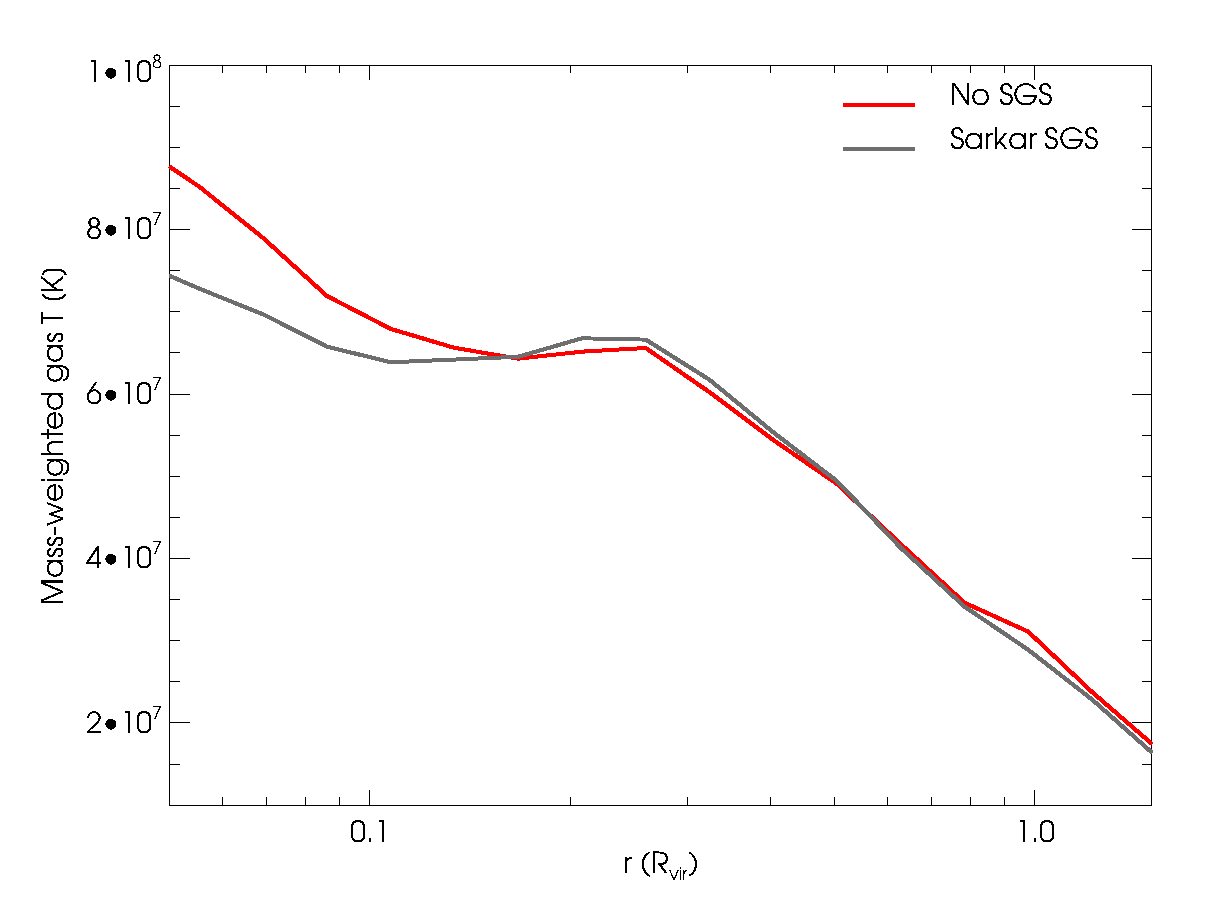
\includegraphics[width=0.45\linewidth]{chapter9/templog.eps}
\label{fig:temp}}
\subfigure[Entropy.]{
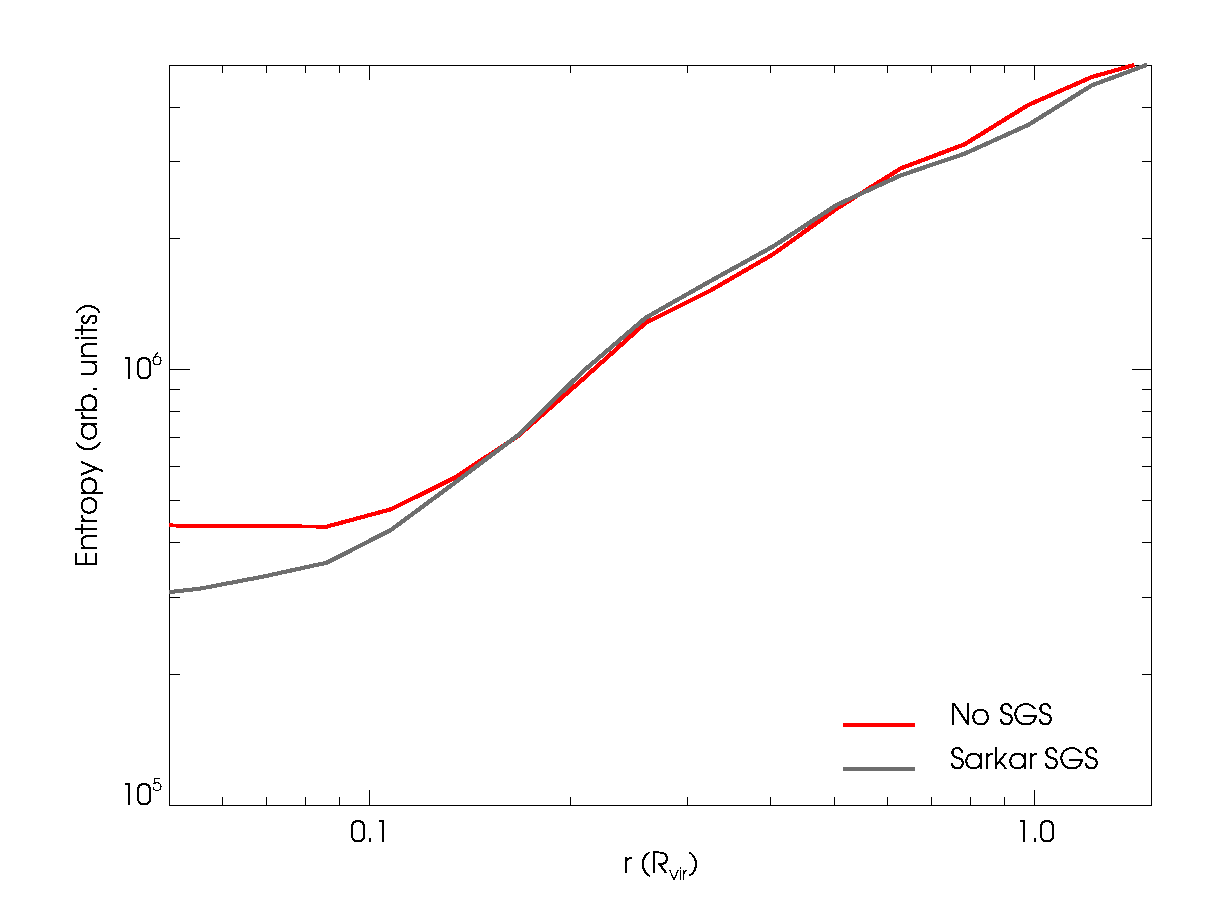
\includegraphics[width=0.45\linewidth]{chapter9/entropylog.eps}
\label{fig:entro}}
\subfigure[X-ray luminosity.]{
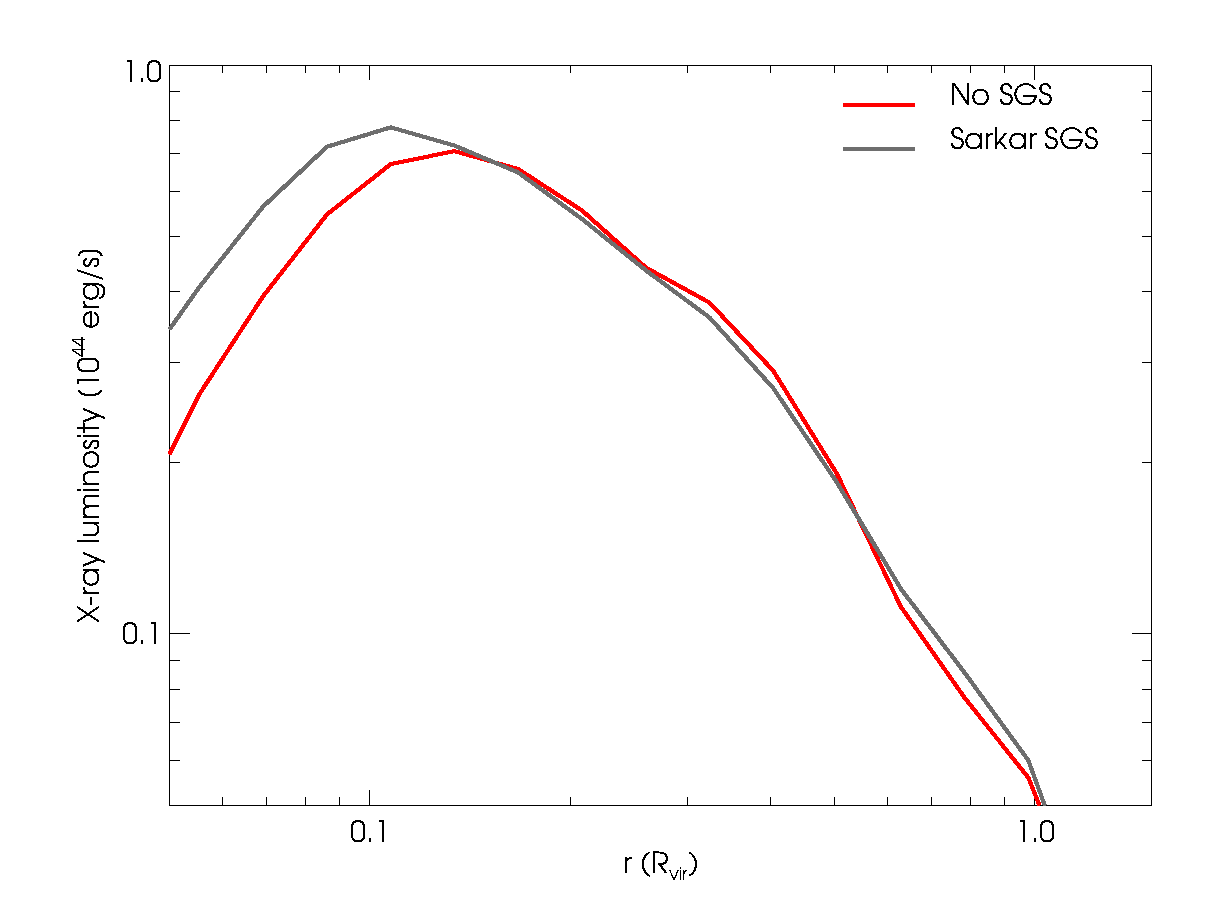
\includegraphics[width=0.45\linewidth]{chapter9/xraylog.eps}
\label{fig:xray}}
\subfigure[Radial profile of effective polytropic index $n_{\text{eff}}(r)$.]{
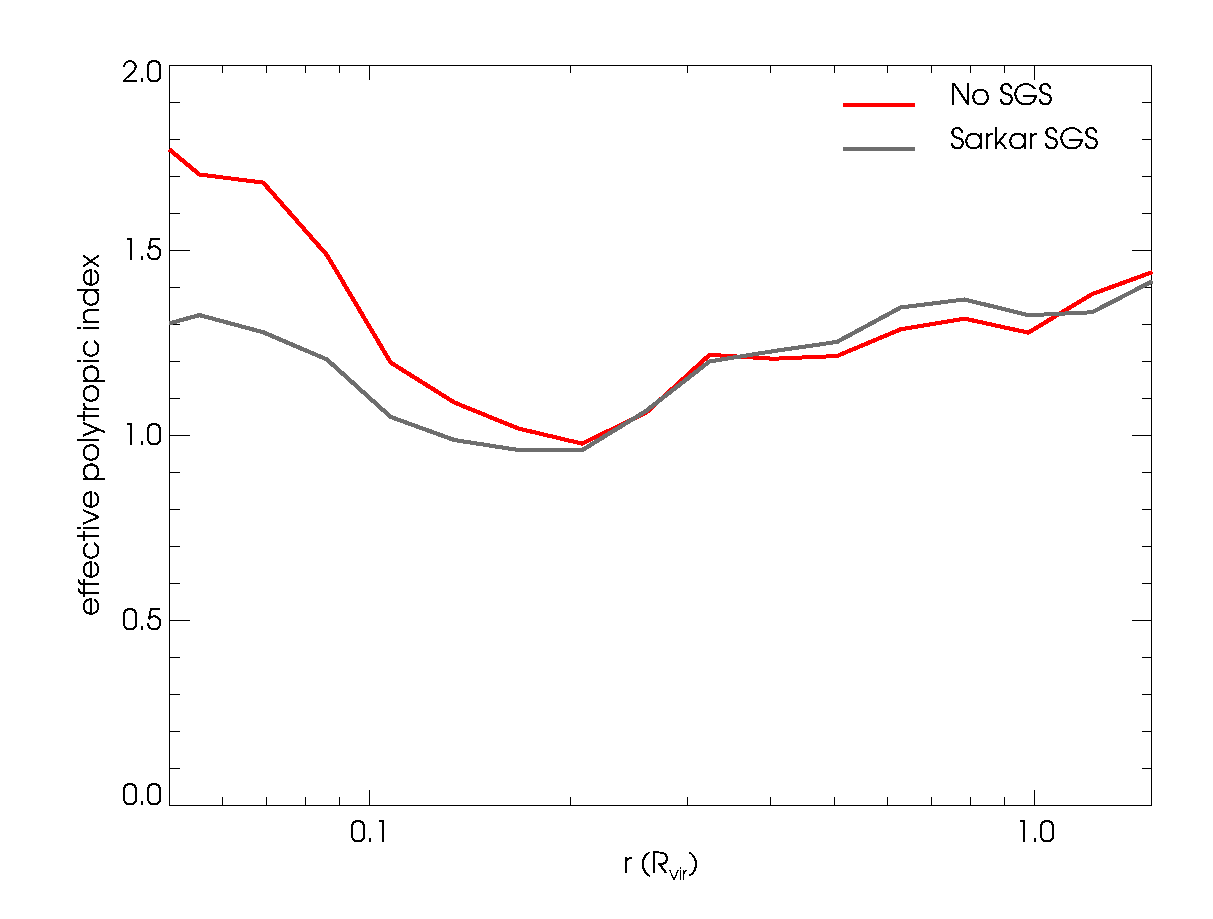
\includegraphics[width=0.7\linewidth]{chapter9/gamma.eps}
\label{fig:poly}}
\caption{Radial profiles of several thermodynamic quantities around the center
of the galaxy cluster. The results for the simulation with and without Sarkar
SGS model are
plotted in red and black respectively.}
\end{figure}
\begin{figure}[tp]
\centering
\subfigure[Radial velocity.]{
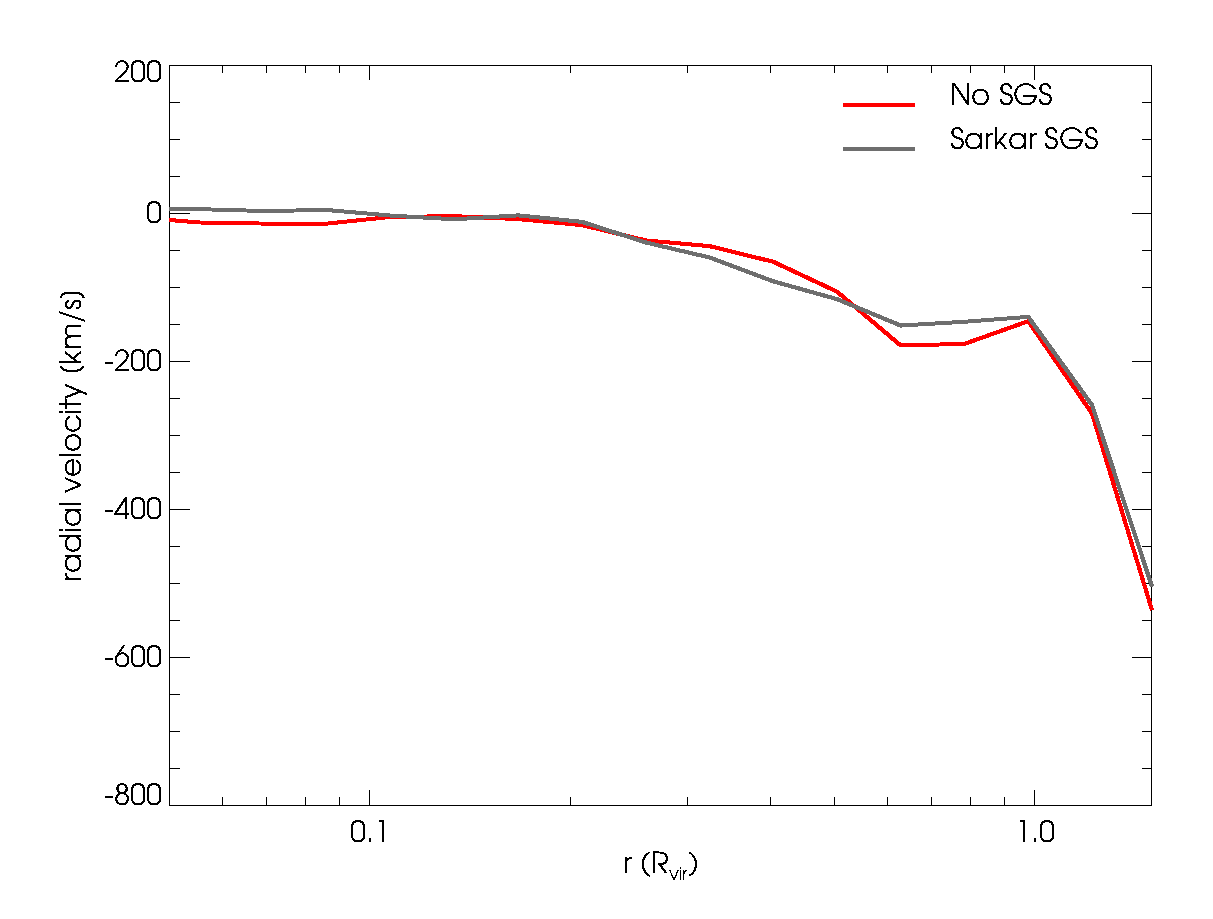
\includegraphics[width=0.45\linewidth]{chapter9/vradlog.eps}
\label{fig:vrad}}
\subfigure[Radial averaged velocity dispersion.]{
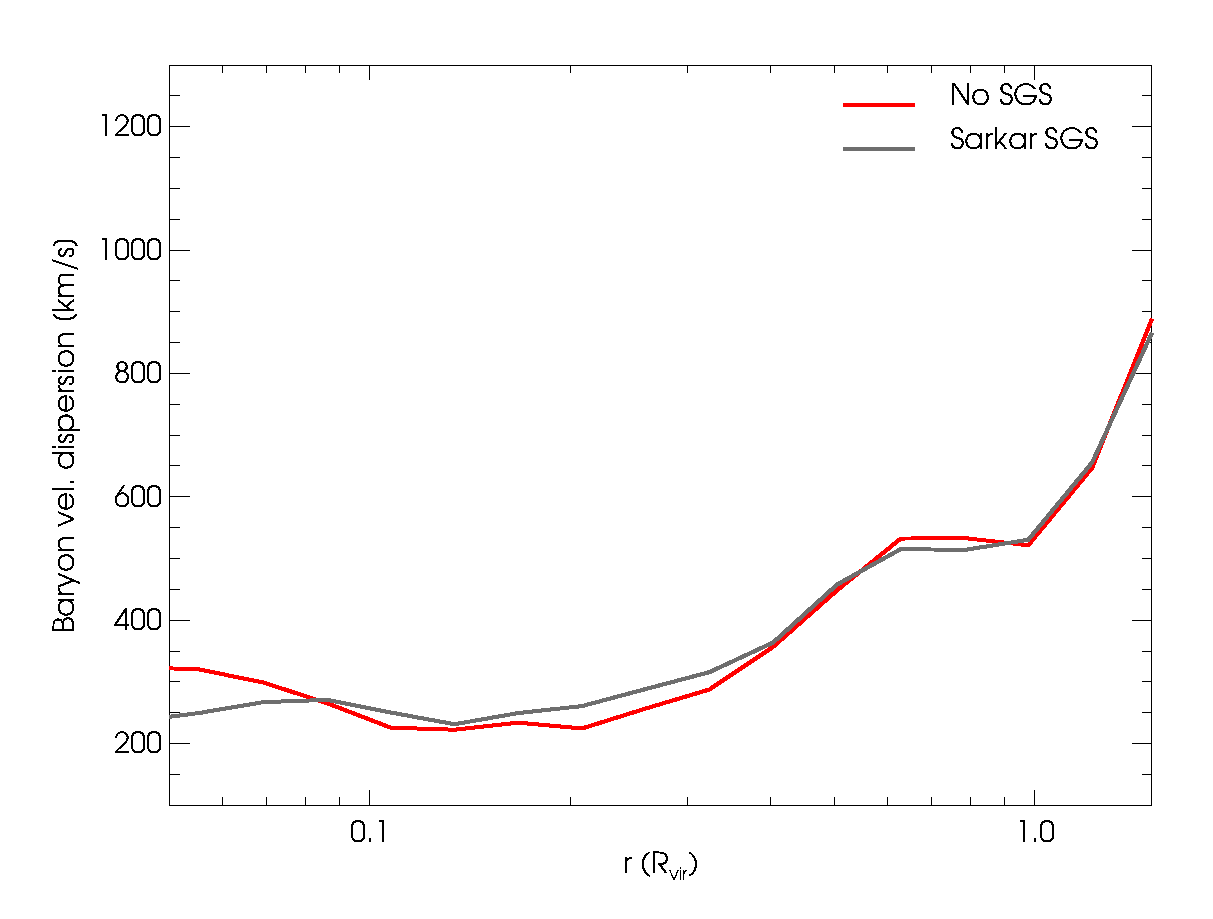
\includegraphics[width=0.45\linewidth]{chapter9/sigma_gaslog.eps}
\label{fig:sigma}}
\subfigure[Scaled turbulent velocity.]{
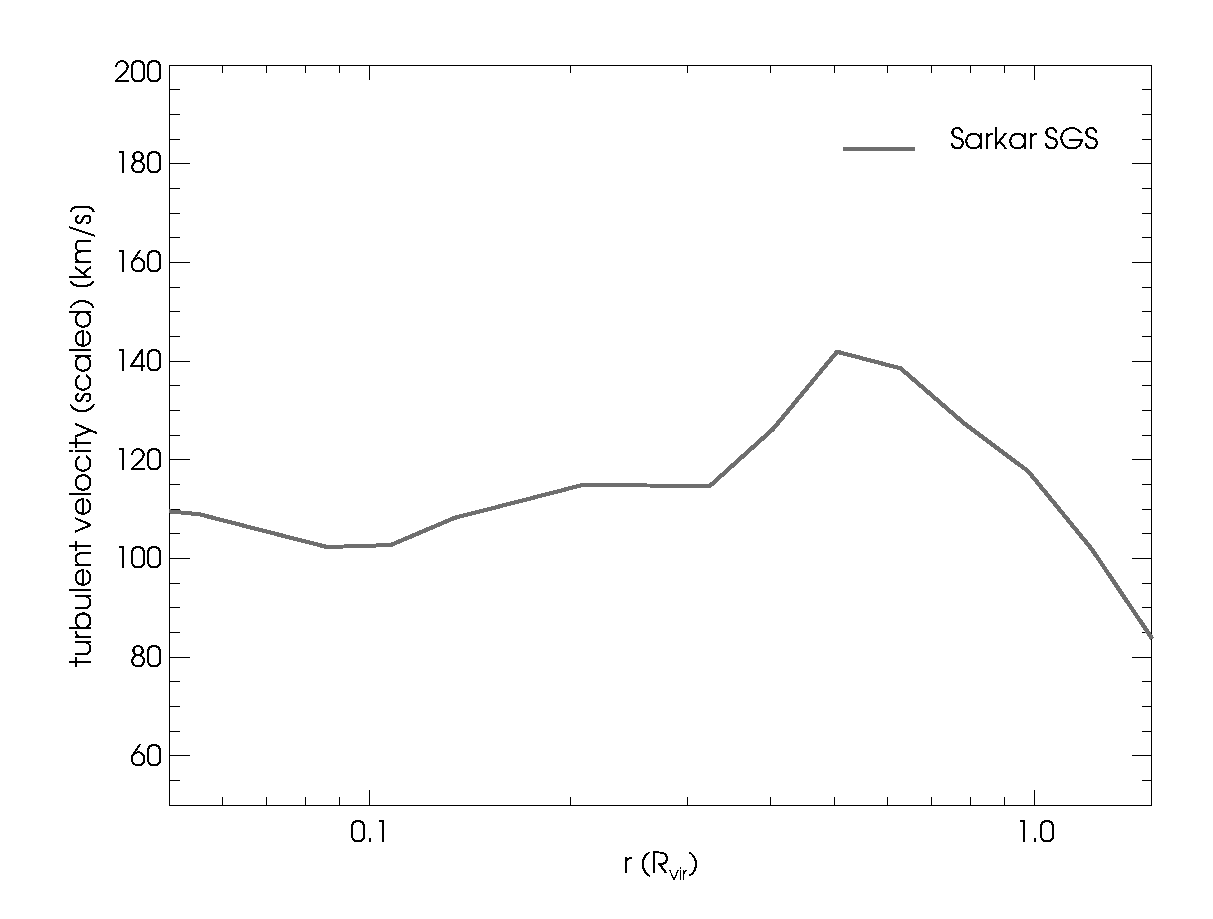
\includegraphics[width=0.7\linewidth]{chapter9/vturblog.eps}
\label{fig:vturb}}
\caption{Radial profiles of several velocity related quantities around the
center of the galaxy cluster. The results for the simulation with and without
Sarkar SGS model are plotted in red and black respectively.}
\end{figure}

The plots show the mass weighted average values at radius $r$ of temperature
$T(r)$ in Kelvin, the density\footnote{The density is not mass weighted
.} $\rho(r)$ in $\unit{M_{\odot}/Mpc^3}$, the scaled turbulent velocity
according to equation \eqref{eq:vturbscaled} $v_t(r)$ in $\unit{km\ s^{-1}}$,
the radial component of the resolved velocity $v_r(r)$ in $\unit{km\ s^{-1}}$,
the entropy $K$ in code units, which is defined as\footnote{This definition of
entropy is often used in literature on galaxy clusters
\citep{Voit2005,Iapichino2008}.}
\begin{align}
K=\frac{T}{\rho^{\gamma-1}}
\end{align}
with $\gamma = 5/3$, the x-ray luminosity $L_X \sim \rho^2 T^{1/2}$ and the
radially averaged velocity dispersion, which is defined as the standard
deviation of the velocity averaged over a spherical shell as
\begin{align}
\sigma(r) = \frac{\sum_i m_i \lra{v_i - \fil{v(r)}}^2}{\sum_i m_i} 
\end{align}
where $\fil{v(r)} = \frac{\sum_i m_i}{\sum_i m_i}$ is the mass weighted mean
value of velocity in the spherical shell at radius $r \pm \delta r$. 

At first it is apparent from these plots that, except for the radial
component of the resolved velocity, the run with SGS model only shows
significant deviations from the run without SGS model in the cluster core at
$r<0.1\ R_{vir}$. However since \texttt{enzo\_anyl} proved not to be
robust for 
$r< 0.07\ R_{vir}$ \citep{Iapichino2008}, one cannot use the values
obtained by these plots for a consistent analysis of the cluster core; this
will be done in the next chapter using a different tool.
Nevertheless the general trend from these plots is, that the SGS model lowers
the entropy in the core, which leads to a higher density and a lower
temperature in the center of the cluster. Since the X-ray luminosity is
proportional to $\rho^2$, it is higher in the cluster core of the simulation
with SGS model. Looking more precisely at the radial profile of entropy
(fig. \ref{fig:entro}), one can also see that in the simulation without the SGS
model, the entropy inside the core of the cluster $r > 0.1\ R_{vir}$ is
basically constant, which suggests that the gas is adiabatic there. With the
SGS model this is not the case; the entropy is falling steadily towards the
center of the core. 

The last observation can be discussed more quantitatively in terms of
polytropic processes. A polytropic process is defined as a process, where
\begin{align}
\frac{T}{\rho^{n-1}} = const.,
\end{align}
where $n$ is called the polytropic index. By reversing that logic we can
compute an effective polytropic $n_{\text{eff}}(r)$ index by demanding that
\begin{align}
\td{r}\lra{\frac{T}{\rho^{n_{\text{eff}}(r)-1}}}=0,
\end{align}
which leads to
\begin{align}
n_{\text{eff}}(r)=\frac{\rho}{T}\frac{\ttd{r}{T}}{\ttd{r}{\rho}}+1
=\ttd{\ln T}{\ln \rho}+1. 
\end{align}
In figure \ref{fig:poly}
we show a plot of the radial dependence of the effective
polytropic index for our two simulations with and without SGS model. 
We see that the polytropic index in the simulation without SGS
model is $n_{\text{eff}} \approx 1.7$, which is near to the adiabatic case
$n_{\text{eff}} \approx 5/3$, as expected. The simulation with SGS model is
clearly not
adiabatic, with $n_{\text{eff}} \approx 1.3 \approx 4/3$ in the center. We
also note that at a radius $r \approx 0.2\ R_{vir}$, the gas behaves
basically
isothermal, which can also be seen in the temperature profile
(figure \ref{fig:temp}). At an even bigger distance from the core 
$r > 0.2\ R_{vir}$, the cluster gas in both simulations behaves similarly,
with a
polytropic index rising from $n \approx 1.3$ to $n \approx 1.4$. 
If we compute an average polytropic index over the region 
$0.05\ R_{vir} < r < 1.0\ R_{vir}$ we get $n_{\text{eff}} = 1.27$
and $n_{\text{eff}} = 1.18$
for the simulation without and with SGS respectively. It is
interesting to compare these values with results from observations. For example 
\citet{Markevitch1998} found that they could fit their measured temperature
profiles with a polytropic index of $n=1.2-1.3$, which would fit reasonably
well to our average values. However, \citet{Pratt2002} claim that 
$n=1.07 \pm 0.1$ is the best fit to their observed temperature profile, and
therefore state, that the whole cluster can be seen as nearly isothermal.
But newer measurements by \citet{Vikhlinin2006} now reveal, that the
temperature profile cannot be fitted by a single polytropic index in agreement
with our analysis. \citet{Vikhlinin2006} also find a broad plateau of
temperature at $r=0.2\ R_{vir}$ in most of their clusters, however all
their
temperature profiles show a decline of temperature towards the center of the
cluster at $r < 0.2\ R_{vir}$, a so-called "cool core". This feature
could
neither be reproduced by the simulation without SGS nor with SGS. It seems like
including turbulence alone in a cluster simulation cannot be a solution to the
"cool core" problem. 

The radial resolved velocity is not changed significantely by
the SGS model, but comparing this plot with the radial profile of the turbulent
velocity the following picture emerges: From a radius $r > R_{vir}$
material is falling onto the cluster, being decelerated strongly at the
virial radius $r = R_{vir}$ (see drop of radial velocity at this point in
figure \ref{fig:vrad}). This deceleration leads to a steady rise in turbulent
energy at $r<R_{vir}$ up to a peak at $r=0.5\ R_{vir}$ followed by a drop of to
a quite stable value of $\sim \unit[110]{km s^{-1}}$ in the region 
$r<0.3\ R_{vir}$. One might want to compare these value to the velocity
dispersion, however these values are not comparable directly. The turbulent
velocity depicted in the plot is computed for the characteristic scale
$\unit[15.7]{kpc\ h^{-1}}$, which is constant with the radius. The velocity
dispersion is the deviation of velocity in a spherical shell at radius $r$, so
the characteristic scale of $\sigma$ is basically the circumference of this
shell
$l=2\pi r$, which is of course not independent of the radius. Therefore we
cannot interpret the value of $\sigma$ in the same local sense as we can do for
the other quantities. We therefore doubt that it is useful to draw conclusions
about the local nature of turbulence from a plot like fig. \ref{fig:sigma}, as
is often done in the literature (e.g. \citep{Norman1999a}). 

\subsection{Spatial distribution of turbulent energy}
To investigate the time development of the spatial distribution of turbulent
energy, we generated slices of density and turbulent energy with the graphical
analysis tool VisIt. 
\begin{figure}[tp]
\centering
\subfigure[$z=0.15$.]{
\includegraphics[width=0.46\linewidth,clip,trim=150 50 50 0]
{chapter9/mergerdens0011.eps}
\label{fig:dens0011}}
\subfigure[$z=0.15$.]{
\includegraphics[width=0.46\linewidth,clip,trim=150 50 50 0]
{chapter9/mergereturb0011.eps}
\label{fig:eturb0011}}
\subfigure[$z=0.1$.]{
\includegraphics[width=0.46\linewidth,clip,trim=150 50 50 0]
{chapter9/mergerdens0012.eps}
\label{fig:dens0012}}
\subfigure[$z=0.1$.]{
\includegraphics[width=0.46\linewidth,clip,trim=150 50 50 0]
{chapter9/mergereturb0012.eps}
\label{fig:eturb0012}}
\caption{Slices of density (left) and turbulent energy at a length scale of
$\unit[15.6] {Mpc\ h^{-1}}$ (right) at varying redshifts $z$. The color coding
shows both quantities in code units using a logarithmic scaling. The overlayed
contours show density and the overlayed vector field depicts the strength and
direction of the baryonic velocity field in code units using a linear scale. The
slices show a 
region of $\unit[6.4 \times 6.4] {Mpc\ h^{-1}}$. }
\end{figure}
\begin{figure}[tp]
\centering
\subfigure[$z=0.05$.]{
\includegraphics[width=0.46\linewidth,clip,trim=150 50 50 0]
{chapter9/mergerdens0013.eps}
\label{fig:dens0013}}
\subfigure[$z=0.05$.]{
\includegraphics[width=0.46\linewidth,clip,trim=150 50 50 0]
{chapter9/mergereturb0013.eps}
\label{fig:eturb0013}}
\subfigure[$z=0$.]{
\includegraphics[width=0.46\linewidth,clip,trim=150 50 50 0]
{chapter9/mergerdens0014.eps}
\label{fig:dens0014}}
\subfigure[$z=0$.]{
\includegraphics[width=0.46\linewidth,clip,trim=150 50 50 0]
{chapter9/mergereturb0014.eps}
\label{fig:eturb0014}}
\caption{Slices of density (left) and turbulent energy at a length scale of
$\unit[15.6] {Mpc\ h^{-1}}$ (right) at varying redshifts $z$. The color coding
shows both quantities in code units using a logarithmic scaling. The overlayed
contours show density and the overlayed vector field depicts the strength and
direction of the baryonic velocity field in code units using a linear scale. The
slices show a region of $\unit[6.4 \times 6.4] {Mpc\ h^{-1}}$. }
\end{figure}
The slices are taken around the place of
formation of our main galaxy cluster and show a region of size 
$\unit[6.4 \times 6.4] {Mpc\ h^{-1}}$. Overlayed onto the slices are density
contour lines and a vector field showing the strength and direction of
the velocity. In the density slice at redshift $z=0.15$
(figure \ref{fig:dens0011}), we can see from the velocity vectors that material
is falling onto the cluster along filament from the lower left and from the
upper right corner. But from the upper right corner we do not have a smooth
inflow of matter, instead two small clumps are approaching. Over the course of
the simulation these two clumps merge with the main cluster
(figure \ref{fig:dens0012}-\ref{fig:dens0012}) and are assimilated completely
at redshift $z=0$. Only the velocity field still shows some disturbance
due to the infalling clumps.  

In the slice of the turbulent energy (figure \ref{fig:eturb0011}) at $z=0.15$,
we see a hot spot of turbulent energy in the center of our cluster, which is due
to a former major merger. The turbulent energy produced due to this merger is
declining (figure \ref{fig:eturb0012}-\ref{fig:eturb0014}) and at redshift
$z=0$ it is presumably dissipated into internal energy completely, so there
is only little turbulent energy left at the center of the cluster. 

However the two approaching clumps will drive turbulence again in the cluster.
Thereby the left clump can be identified in the turbulent energy slice at
$z=0.15$ (figure \ref{fig:eturb0011}) as a ring-like structure, showing that
turbulence is not produced in the center of the infalling clump, but is
presumably produced at the front (behind a 
bow shock) and in the wake of the infalling material. But the right clump only
shows some turbulence production in its wake, which might be due to its smaller
size and smaller velocity. However, on their way towards the main cluster, both
clumps develop a hot spot of turbulent energy (figure
\ref{fig:eturb0012}-\ref{fig:eturb0013}). The hot spot of turbulent energy can
even be identified after the two clumps have merged with the main cluster
(figure \ref{fig:eturb0014}) and are not visible in the density slice (figure
\ref{fig:dens0014}) anymore. In this sense,
the distribution of turbulent energy traces the local merging history of a
galaxy cluster until it is dissipated into heat completely. Also the merging of
the two small clumps with the main cluster drives turbulence only in its
outer rim, showing that smaller mergers might only be able to drive turbulence
in the outer regions ($r > R_{vir}$) of a cluster. But turbulence is
sustained for a longer time in a galaxy cluster than one might expect from just
looking at density development.

\subsection{Cluster core analysis}
As mentioned we couldn't use the \texttt{enzo\_anyl} tool to compute average
values of
thermodynamic quantities of the cluster core. Instead we analyzed the cluster
core using the interactive parallel visualization and graphical analysis tool
VisIt\footnote{Freely available from https://wci.llnl.gov/codes/visit.}. Using
this tool we computed several mass-weighted averaged quantities within a sphere
of radius $R=0.1\ R_{vir}$, centered at the cluster center. The results of this
analysis are summarized in tables
\ref{tab:avg}\subref{tab:avg1}-\ref{tab:avg}\subref{tab:avg3}.
\begin{table}[tp]
\begin{center}
\begin{small}
\subtable[General quantities.]{
\begin{tabular}{lccccc}
\hline
Run & $m_{bar}$ & $\rho$ & $T$ & $K$ & $\sigma$\\
& $[\unit[]{10^{12}\ M_{\odot}}]$
& $[\unit[]{10^{14}\ M_{\odot}\ Mpc^{-3}}]$
& $[\unit[]{10^7\ K}]$
& $[\unit[]{10^5 \times code\ units}]$
& $[\unit[]{km\ s^{-1}}]$\\
\hline
no SGS & 2.73 & 0.996 & 7.88 & 4.40 & 200\\
SGS & 3.37 & 1.29 & 6.99 & 3.38 & 257\\
\hline
\end{tabular}
\label{tab:avg1}
}
\\
\subtable[Resolved and thermal pressure.]{
\begin{tabular}{lccccc}
\hline
Run 
& $p_{th}/\rho$ 
& $p_{res}/\rho$ 
& $\frac{p_{res}}{p_{th}+p_{res}}$\\
& $[\unit[]{10^{16}\ cm^2 s^{-2}}]$
& $[\unit[]{10^{14}\ cm^2 s^{-2}}]$
& $[\unit[]{\%}]$\\
\hline
no SGS & 1.05 & 1.34 & 1.25\\
SGS & 0.936 & 2.20 & 2.30\\
\hline
\end{tabular}
\label{tab:avg2}
}
\\
\subtable[SGS quantities.]{
\begin{tabular}{lccccc}
\hline
Run 
& $p_{turb}/\rho$ 
& $\epsilon$ 
& $\Sigma$\\
& $[\unit[]{10^{14}\ cm^2 s^{-2}}]$
& $[\unit[]{10^{-5}\ cm^2 s^{-3}}]$
& $[\unit[]{10^{-5}\ cm^2 s^{-3}}]$\\
\hline
no SGS & 0.0 & 0.0 & 0.0\\
SGS & 0.380 & 3.06 & 2.92\\
\hline
\end{tabular}
\label{tab:avg3}
}
\end{small}
\end{center}
\caption{Mass weighted values of some quantities, calculated
within a sphere with $R = 0.1\ R_{vir}$ centred at the cluster center at
z=0.}
\label{tab:avg}
\end{table}
The table lists as general quantities of the simulations the baryonic mass
$m_{bar}$ inside the chosen sphere, the density $\rho$, the temperature $T$, the
entropy $K=\frac{T}{\rho^{\gamma-1}}$ with $\gamma=5/3$ and the baryonic
velocity dispersion $\sigma= \frac{\sum_i m_i \lra{v_i -
\fil{v}}^2}{m_{bar}}$ at the length scale 
$l=0.1\ R_{vir}=\unit[133]{kpc\ h^{-1}}$. According to \citet{Voit2005} entropy
is the most important quantity to look at, because it determines
the structure of the intracluster medium and it records the thermodynamic
history of the cluster's gas; the temperature and density are just
manifestations of the entropy.
We find that the ratio of the entropies in the cluster core of the two
simulations (in the 
following 1 is used to subscript quantities of the run without SGS model, 2
subscripts quantities of the simulation with SGS model) is
\begin{align}
\frac{K_1}{K_2}=1.30 = \lra{\frac{\rho_1}{\rho_2}}^{-1}=
\lra{\frac{\sigma_1}{\sigma_2}}^{-1}.
\end{align}
Since $\frac{K_1}{K_2}=
\lra{\frac{T_1}{T_2}}\lra{\frac{\rho_1}{\rho_2}}^{-2/3}$ by definition, this
yields
\begin{align}
\lra{\frac{T_1}{T_2}}=\lra{\frac{\rho_1}{\rho_2}}^{-1/3}=1.09,
\end{align}
which is roughly fulfilled, since from the data directly
we get $T_1/T_2 = 1.13$. So temperature and density are really just
manifestations of entropy, but also the velocity dispersion of the baryonic
gas in the cluster core seems to be directly connected to the entropy.
Because of this, the velocity dispersion at a length scale of $l=0.1\ R_{vir}$
in
the simulation with the SGS model is significantely higher than in the
simulation without SGS model.

In table \ref{tab:avg2} we list the thermodynamic pressure $p_{th}$ and the
resolved pressure, which is defined as
\begin{align}
p_{res}=\frac{1}{3} \rho \sigma^2,
\end{align}
and the ratio between resolved and thermodynamic pressure. We see that, in 
the case of the SGS model simulation, the ratio of resolved to thermal pressure
is nearly twice as high compared to the simulation without SGS model, since
density and velocity dispersion are higher in the core when using the SGS
model.

Listed in table \ref{tab:avg3} is also the turbulent pressure, defined as
\begin{align}
p_{res}=\frac{1}{3} \rho q^2,
\end{align}
where $q^2$ is related to the velocity fluctuations at grid length scale 
$l=\unit[15.7]{kpc\ h^{-1}}$. So directly comparing or adding the resolved
pressure to the turbulent pressure is not useful, since both are related to the
deviations of the velocity on different length scales. However,
the ratio of turbulent production $\Sigma$ to turbulent dissipation $\epsilon$
in the core of the cluster is interesting
\begin{align}
\frac{\Sigma}{\epsilon}=0.95,
\end{align}
showing that we are actually in a regime of near equilibrium of production and
dissipation of turbulent energy, a sign that a turbulent cascade has
established.

\subsection{Influence of SGS parameters on cluster core}
In an attempt to better understand the influence of the SGS model on the
thermodynamic properties of the cluster core, we conducted a series of
simulations with different parameters for the SGS model. Because of our
restricted CPU budget we could not afford to do these simulations with the full
$128^3$ root grid resolution, rather we were only able to do these studies using
a
root grid resolution of $32^3$ grid cells and $32^3$ N-body particles. In
analogy to the high resolution simulation, we also nested a static child grid
inside the root grid, with $32^3$ cells and $32^3$ N-body particles. The mass
of each particle in this grid was $\unit[5.8 \times 10^{11}]{M_{\odot}\
h^{-1}}$,
so the resolution of the gravitational potential due to dark matter was much
lower in these runs. We allowed adaptive grid refinement from level
$l=2$ to $l=8$ in a volume of $\unit[38.4]{Mpc\ h^{-1}}$ inside this grid, so
the effective resolution of the baryonic component and all the other
parameters were equal to the high resolution runs.
The galaxy clusters that formed in these simulations had a virial mass of
roughly $M_{vir}=\unit[6.9 \times 10^{14}]{M_{\odot}\ h^{-1}}$ and a virial
radius
of $R_{vir}=\unit[1.27]{Mpc\ h^{-1}}$.

\begin{figure}[tp]
\centering
\subfigure[Linear scaling.]{
\includegraphics[width=0.45\linewidth]{chapter9/epsfitturb.eps}
\label{fig:epsfit}}
\subfigure[Logarithmic scaling.]{
\includegraphics[width=0.45\linewidth]{chapter9/epsfitturblog.eps}
\label{fig:epsfitlog}}
\caption{Plot of turbulent pressure over density versus turbulent dissipation
in the center of the cluster core for different parameters of the SGS model.}
\end{figure}

As parameters we chose all combination of $C_{\nu} = (0.0, 0.05),
C_{\lambda}=(0.0,-0.2),C_{\mathbb{D}}=(0.0,0.4)$ and $C_p =
(0.0,1.0)$\footnote{Setting $C_p=0.0$ means switching off
the influence of the turbulent pressure in the momentum equation.}, which 
gave use 16 combinations altogether. In complete analogy to the high resolution
runs we analyzed the average values of thermodynamic quantities of the cluster
core. Albeit one interesting preliminary result emerged. By plotting the 
average values of the turbulent pressure over the average value of turbulent
dissipation in the cluster core (figures \ref{fig:epsfit},\ref{fig:epsfitlog}),
we found that they seem to be related as
\begin{align}
\fil{\frac{p_t(l_{min})}{\rho}} = 
C (\fil{\epsilon} R_{vir})^{2/3},\label{eq:turbeos}
\end{align}
where $\fil{}$ means the mass weighted average over the cluster core
$r<0.1\ R_{vir} $, $l_{min}=\unit[15.6]{kpc\ h^{-1}}$ and $R_{vir} =
\unit[1.27]{Mpc\ h^{-1}}$. The constant $C$ can be found
from a linear fit to be $C \approx 1$ (see fit in figures
\ref{fig:epsfit},\ref{fig:epsfitlog}).
If we use again our scaling relation for the
turbulent velocity \eqref{eq:vturbscaled}, we get with
$\fil{\frac{p_t(l_{min})}{\rho}} = \fil{q^2(l_{min})}$ and $C=1$
\begin{align}
\fil{q^2(l)} = \lra{\frac{R_{vir}}{l_{min}}}^{2/3} \fil{\epsilon}^{2/3} l^{2/3}
\end{align}
If we assume, that the value of $\frac{R_{vir}}{l_{min}}^{2/3} = 18.8$ is
universal, we get for cluster core turbulence the relation
\begin{align}
\fil{q^2(l)} = 18.8 \fil{\epsilon}^{2/3} l^{2/3}.
\end{align}
In this sense, we can interpret $C_{k,core}=18.8$ as a Kolmogorov constant for
the cluster core turbulence, which is more than 10 times higher than what is
found for the Kolmogorov constant in simulations of incompressible turbulence.



\chapter{Summary and Conclusions}\label{summ}
Turbulence is often invoked in astrophysics to explain phenomena, which are
not understood. However, studies that quantify the real impact of 
turbulence in astrophysical environments in general, or especially for the
formation of galaxy clusters, are not available. One reason for this is
obviously the lack of an accepted theory of compressible and/or supersonic
and/or
selfgravitating turbulence. A second reason is that the models used to
describe numerically the influence of turbulence (so-called 
large-eddy-simulations) are based on the notion of
filtering the fluid dynamic equations at a specific length scale, which is
incompatible with adaptive grid codes used to study astrophysical phenomena.

The aim of this work was to address the second problem, thereby developing,
implementing, and applying a new numerical scheme for modeling turbulent flows
over a great range of length scales suitable to treat astrophysical flows in
galaxy cluster cores or star forming regions. Because the cosmological fluid
code Enzo uses blockstructured adaptive mesh refinement in combination with
a low dissipative PPM-Solver, it was a natural choice to implement our ideas
into this code.

Still, great technical and numerical difficulties had to be circumvented.
Nevertheless, we could finally show that the
idea of our $\epsilon$-based approach to correct the velocity and energy fields
at grid refinement/derefinement according to local Kolmogorov scaling can
produce consistent results in simulations of driven turbulence. We demonstrated
that energy conservation and the scaling of turbulent energy in our adaptive
simulations is consistent with static grid simulations. 

Motivated by these results, we then attempted to use our new numerical scheme in
 simulations of galaxy cluster formation. Two high resolution runs of galaxy
cluster formation, one with and one without a turbulence model, have been
conducted to explore the influence of
turbulence modeled with our scheme on the formation of galaxy clusters. From
the analysis of these simulations, we conclude the following:
\begin{itemize}
\item Our turbulence model seems to have no significant influence on the mass
fractions of different gas phases of the ICM. 
\item The time development of turbulent energy in the simulation suggests that
basically all gas phases of the intracluster medium had enough time to develop
a turbulent cascade. In fact, we could show that our model seems to be near an
equilibrium of production and dissipation of turbulence, especially in the
cluster core. 
\item The turbulence at a length scale of galaxies 
($\approx \unit[10]{kpc\ h^{-1}}$) is subsonic, and the average
turbulent Mach number at these scale is found to be $0.2$ at redshift $z=0$. 
\item In the beginning of galaxy cluster formation great fluctuations of
turbulent energy can be seen, suggesting that violent merging can produce a
substantial amount of turbulence. 
\item Minor mergers can drive turbulence only at the outer rim 
($r>R_{vir}$) of the galaxy cluster. The spatial distribution of turbulent
energy traces the local merging history of a galaxy cluster until the turbulent
motions are dissipated into heat completely. 
\item From the scaling properties of turbulent energy it seems that energy
is injected at a scale of $\approx \unit[100]{kpc\ h^{-1}}$ cascading down to
smaller scales. From the radial profile of our cluster we found a peak of
turbulent energy at $r=0.5\ R_{vir}$, probably produced by the infall and 
strong deceleration of material, when it hits the virial boundary of the
cluster.
\item From the radial profiles of several thermodynamical quantities of the
galaxy cluster it is evident, that only inside the core ($r<0.1\ R_{vir}$)
can one find a significant influence of our turbulence model. The radial profile
of
the effective adiabatic index shows that the influence of the turbulent model
can be described as a kind of cooling, leading to lower entropy, lower
temperature, and therefore higher gas density and higher velocity dispersion in
the core. "Cooling" due to turbulence does not lead to an overcooling
problem, but it is not strong enough to explain the cool cores of galaxy
clusters.
\end{itemize}

The last result begs the question of how turbulence would influence a
simulation of cluster formation including cooling. If there is no nontrivial
interaction between cooling and the turbulence model, our results indicate that
turbulence would even enhance the overcooling problem in the core. So
suggesting turbulence as a heating mechanism that prevents galaxy cluster
cores from overcooling seems to be problematic. Nevertheless more
simulations of galaxy clusters, including different physics have to
be carried out to confirm our results. 

Interestingly preliminary results from low resolution simulations suggest, that
turbulent velocity in the cluster core obeys a Kolmogorov scaling law with
a Kolmogorov constant more than 10 times higher than in incompressible
simulations. Whether this finding is only a feature of our SGS model
or a universal feature of turbulence in the cluster core should be
investigated in the future.

More attention should also be given to the fact that turbulent energy and
thus unresolved turbulent velocity fluctuations are scale dependent. It is
often claimed in the astrophysical literature that the amount of
turbulence is a certain fraction of thermal energy or kinetic energy, without
specifying the length scale for which this statement was made. In the spirit of
Kolmogorov theory of turbulence, such statements are incomplete. This is
especially apparent in our adaptive grid simulations, where different grid
length scales at the same time are used to describe a flow. However, we have to
note that the idea of scale dependent velocity fluctuations poses
difficult conceptual problems. For example, the mass inside a certain radius $r$
from the equation of hydrostatic equilibrium is, including turbulent pressure,
also scale dependent\footnote{For a derivation see appendix \ref{stat}.}
\begin{align}
M(r,l) &= - \frac{r}{G} 
\lrb{R_s T_g \lra{\ppd{\ln r}{\ln T_g}+\ppd{\ln r}{\ln \rho_g}}
+\frac{q^2(l)}{3}\lra{\ppd{\ln r}{\ln q^2(l)}+\ppd{\ln r}{\ln \rho}}},
\end{align}
a fact, which is often overlooked. Arguing that turbulent pressure might
explain deviation from the mass found by estimates based on the hydrostatic
equilibrium, is therefore not advisable.

Nevertheless, it might also come out, that the ideas of Kolmogorov and scale
dependent velocity fluctuations are not useful in an astrophysical context.
Within
our work, we only showed how the influence of turbulence obeying basically
Kolmogorov scaling can be numerically treated and what kind of results can be
expected. We could not prove that turbulence in an astrophysical environment
really can be described in this way. Theoretically, Kolmogorov derived
his celebrated result assuming a forcing of turbulence restricted to the largest
length scales, so that in the limit of infinite Reynolds numbers an undisturbed
cascade down to smaller scales can develop. However, gravity is a force acting
on
all length scales, in contradiction to the ideas of Kolmogorov and our
turbulence model. A better understanding of selfgravitating turbulence is
therefore extremely important for the future of turbulence research in
general. 
That's why in the future comparisons between direct numerical simulations of
selfgravitating gas and simulations with our subgrid model should be conducted.
If these simulations support our SGS model (which would also show, that
Kolmogorov scaling is more universal than theory suggests), we can be
confident in saying, that with our FEARLESS ansatz we developed a unique tool
for describing turbulence which aside from cluster physics will lead to many
other applications in astrophysics.  



\appendix
\chapter{Dimensional analysis}\label{dimanal}
We want to write down the general equations of fluid dynamics in dimensionless
form. Therefore we introduce the following dimensionless quantities
\begin{align*}
r_i^*=\frac{r_i}{l_0} &\Rightarrow
\pd{r_i}=\pd{r_i^*}\ppd{r_i}{r_i^*}=\frac{1}{l_0}\pd{r_i^*},\\
v_i^*=\frac{v_i}{v_0},\\
t^*=\frac{t}{l_0} &\Rightarrow
\pd{t}=\pd{t^*}\ppd{t}{t^*}=\frac{1}{t_0}\pd{t^*},\\
\rho^*=\frac{\rho}{\rho_0}.
\end{align*}
Inserting these into the continuity equation \eqref{eq:mass} we get
\begin{align*}
\frac{\rho_0}{t_0}\pd{t^*}\rho^* 
+ \frac{v_0 \rho_0}{l_0} \pd{r_j^*}(v_j^*\rho^*) &= 0 \ | 
\cdot \frac{l_0}{\rho_0 v_0},\\
\underbrace{\frac{l_0}{v_0 t_0}}_{Sr}\pd{t^*}\rho^* 
+ \pd{r_j^*}(v_j^*\rho^*) = 0.
\end{align*}
This derivation shows that solutions of the continuity equation
are similar, if the Strouhal number $Sr = \frac{l_0}{v_0 t_0}$ is the
same. Flows with a Strouhal number $Sr=0$ are so called stationary flows.
Nevertheless, the Strouhal number is most often set to one, by assuming
$v_o=\frac{l_0}{t_0}$. 
Using the additional dimensionless quantities
$p^*=\frac{p}{p_0},\sigma_{ij}^*=\frac{\sigma_{ij}}{\sigma_0},
g^*=\frac{g}{g_0 }$
in the momentum equation \eqref{eq:mom} yields
\begin{align*}
\frac{\rho_0 v_0}{t_0}\pd{t^*}(\rho^* v_i^*) 
+ \frac{\rho_0 v_0^2}{l_0}\pd{r_j^*}(v_j^* \rho^* v_i^*) &= 
- \frac{p_0}{l_0}\pd{r_i^*}p^* 
+\frac{\sigma_0}{l_0}\pd{r_j^*}\sigma_{ij}^*
+\rho_0 g_0 \rho^* g_i^*\ | \cdot \frac{l_0}{\rho_0 v_0^2},\\
\underbrace{\frac{l_0}{v_0 t_0}}_{Sr}\pd{t^*}(\rho^* v_i^*) 
+ \pd{r_j^*}(v_j^* \rho^* v_i^*) &= 
-\underbrace{\frac{p_0}{\rho_0 v_0^2}}_{Ma^{-2}_{iso}}\pd{r_i^*}p^* 
+\underbrace{\frac{\sigma_0}{\rho_0 v_0^2}}_{Re^{-1}}\pd{r_j^*}\sigma_{ij}^*
+\underbrace{\frac{\rho_0 g_0 l_0}{\rho_0 v_0^2}}_{Fr^{-1}} \rho^* g_i^*.
\end{align*}
The occurring dimensionless numbers are the isothermal Mach number $Ma_{iso}$,
which is related to the Euler number $Eu$ or the Ruark number $Ru$ like
$Ma^2_{iso}=Eu=Ru^{-1}$, the Froude number $Fr$, which is related to the
Richardson number $Ri$ like $Fr=Ri^{-1}$ and the Reynolds number $Re$.
All these numbers measure the importance of the term they are related to
compared to the nonlinear advection term $\pd{r_j^*}(v_j^* \rho^* v_i^*)$,
e.g. for high Mach numbers, the pressure term $\pd{r_i^*}p^*$ becomes less and
less important compared to the advection term; for high Reynolds numbers the 
stress term $\pd{r_j^*}\sigma_{ij}^*$ becomes less and less important compared
to the advection term, and the equation shows more and more nonlinear behavior.
For a newtonian fluid with
\begin{align}
\sigma_{ij} \simeq \eta \ppd{r_j}{v_i} = 
\frac{\eta_0 v_0}{l_0} \eta^* \ppd{r_j^*}{v_i^*},
\end{align}
where we introduced the dimensionless quantity $\eta^*=\frac{\eta}{\eta_0}$,
we get $\sigma_0= \frac{\eta_0 v_0}{l_0}$ and therefore we can express the
Reynolds number\footnote{We neglected the second viscosity $\zeta$. In 
principle there exists a second Reynolds number $Re_2=\frac{\rho_0 l_0 v_0
}{\zeta_0}$.} like
\begin{align}
Re=\frac{l_0 \rho_0 v_0^2 }{\eta_0 v_0} = \frac{\rho_0 l_0 v_0 }{\eta_0}.
\end{align}
Playing the same game with the equation for the internal energy 
\begin{align}
\pd{t} \rho e_{int} + \pd{r_j} v_j \rho e_{int} = T \lra{\pd{t} \rho s +
\pd{r_j} v_j \rho s} -p \pd{r_j} v_j \label{eq:eint}
\end{align}
using $e_{int}^*=\frac{e_{int}}{u_0}$ we get
\begin{align*}
\underbrace{\frac{l_0}{v_0 t_0}}_{Sr} \pd{t^*}\rho^* e_{int}^* 
+ \pd{r_j^*} v_j^* \rho^* e_{int}^* &= 
-\underbrace{\frac{p_0}{\rho_0 u_0}}_{Ga_1} p^*\pd{r_j^*}v_j^*
+\underbrace{\frac{\sigma_0}{\rho_0 u_0}}_{Ga_2} \sigma_{ij}^* \pd{r_j^*}v_i^*.
\end{align*}
The new dimensionless quantities that occur in the energy equation seem to have
no name in the literature, but we will call them "Gamma1" (Ga1) and "Gamma2"
(Ga2) for now, since they are related to the adiabatic coefficient.
This can be seen by replacing $p_0 p^*$ according to equation
\begin{align}
p_0 p^* = (\gamma-1) \rho_0 u_0 \rho^* e_{int}^*,
\end{align}
which is valid for an an ideal, nonisothermal ($\gamma \neq 1$) gas. Doing this
we get\footnote{We cannot get rid of Ga2 in the same way, since therefore we
would have to assume an equation relating $\sigma_0 \sigma_{ij}^*$ to the
internal energy. But this would only be possible, if we would assume that the
internal energy is a tensorial quantity, which is not the way how
internal energy is defined normally.}
\begin{align*}
 Sr \cdot \pd{t^*}\rho^* e_{int}^* 
+ \pd{r_j^*} v_j^* \rho^* e_{int}^* &= 
-(\gamma-1) \rho^* e_{int}^* \pd{r_j^*}v_j^*
+Ga_2 \cdot \sigma_{ij}^* \pd{r_j^*}v_i^*.
\end{align*}
For a selfgravitating fluid we even have on more dimensionless quantity, which
appears, when we write down the dimesionless form of the Poisson equation of
gravity
\begin{align}
\underbrace{\frac{g_0}{4\pi G \rho_0 l_0}}_{C_G}\ppd{r_i^*}{g_i^*} = \rho^*.
\end{align}
But this quantity $C_G$ also seems to have no name in the literature
\citep[e.g.][]{Durst2007}.


\chapter{Properties of second order tensors}
A second order tensor can be decomposed into a symmetric and an antisymmetric
part in the following way
\begin{align}
T_{ij}=\underbrace{\frac{1}{2}\lra{T_{ij}+T_{ji}}}_{\text{symmetric}}
+\underbrace{\frac{1}{2}\lra{T_{ij}-T_{ji}}}_{\text{antisymmetric}}.
\end{align}
It can also be decomposed into an isotropic and deviatoric part by subtracting
and adding the trace of the tensor like
\begin{align}
T_{ij}=\underbrace{\frac{1}{n}\delta_{ij} T_{kk}}_{\text{isotropic}}
+\underbrace{T_{ij}-\frac{1}{n}\delta_{ij} T_{kk}}_{\text{deviatoric, 
tracefree}}.
\end{align}
Combining these two relations yields the general decomposition
\begin{align}
\begin{split}
T_{ij}=&
\overbrace{\frac{1}{n}\delta_{ij} T_{kk}}^{\text{isotropic}}
+
\overbrace{
\underbrace{\frac{1}{2}\lra{T_{ij}+T_{ji}-\frac{2}{n}\delta_{ij}
T_{kk}}}_{\text{symmetric, tracefree}}
+\frac{1}{2}\lra{T_{ij}-T_{ji}}}^{\text{deviatoric, tracefree}}\\[-1em]
&\underbrace{\hphantom{\frac{1}{n}\delta_{ij}
T_{kk}+\frac{1}{2}\lra{T_{ij}+T_{ji}-\frac{2}{n}\delta_{ij}
T_{kk}}}}_{\text{symmetric}}
\hphantom{+}
\underbrace{\hphantom{\frac{1}{2}\lra{T_{ij}-T_{ji}}}}_{\text{
antisymmetric}}.
\end{split}
\end{align}

An interesting relation can be found when computing the contraction of a
unsymmetric tensor $U_{ij} \neq U_{ji}$ with a  symmetric tensor
$V_{ij}=V_{ji}$
\begin{align}
U_{ij}V_{ij}
= \frac{1}{2} U_{ij}V_{ij} + \frac{1}{2} U_{ji}V_{ji} 
= \frac{1}{2} U_{ij}V_{ij} + \frac{1}{2} U_{ji}V_{ij}
= \frac{1}{2} \lra{U_{ij}+U_{ji}} V_{ij}.
\label{eq:uscontr}
\end{align}
In analogy one finds for the contraction of an unsymmetric tensor $U_{ij}$ with
an
antisymmetric tensor $W_{ij}=-W_{ji}$
\begin{align}
U_{ij}W_{ij} = \frac{1}{2} \lra{U_{ij}-U_{ji}} W_{ij}.
\label{eq:uascontr}
\end{align}

\chapter{Derivation of the stress tensor for a newtonian fluid}\label{stress}
We derive the stress tensor by considering the dissipation of a motionless
fluid seen by a rotating observer. This derivation is different from what
is found in the literature \citep[eg.][]{Greiner1991} and therefore presented
here.

It is generally assumed that friction between fluid elements is proportional
to the area of their surfaces. So in general the frictional or viscous force
on a fluid element can be expressed like
\begin{align}
F_{visc,i}= \oint_A \sigma'_{ij} n_j dA = \int_V \pd{r_j} \sigma'_{ij} dV.
\end{align}
This force leads to an irreversible rise of temperature in the fluid or an
irreversible
decrease of kinetic energy expressed by the equation for the
dissipation\footnote{See \citet{Landau1991}.}
\begin{align}
\pd{t} E_{kin,visc} = - \int_V \sigma'_{ij} \pd{r_j} v_i dV.
\end{align}
For a motionless fluid ($v_i=0$) and for a fluid with constant velocity 
($\ppd{r_j}{v_i} = 0$) this integral is zero. But also a rotating observer
of a motionless fluid should not see a rise in the temperature of a fluid
\footnote{We do not consider here the a rigidly rotating fluid as is often
done in the literature, because a rigidly rotating fluid is unphysical. This is
so, because a rigidly rotating fluid can never fulfill the
boundary condition $v_i=0$. However, for a rotating observer, the boundary
is also rotating, so that the boundary condition for a boundary at distance $R$
is
$v_i=\epsilon_{ijk}\omega_j R_k$ and there is no contradiction to the velocity 
field \eqref{eq:rotfield}.}
that means
\begin{align}
 \int_V \sigma'_{ij} \pd{r_j} v_i dV = 0 .\label{eq:nodiss}
\end{align}
A rotating observer of a motionless fluid sees a velocity field of the form
\begin{align}
v_i=\epsilon_{ijk}\omega_j r_k \label{eq:rotfield}.
\end{align}
where $\omega_j$ is the angular velocity vector and $r_k$ is the position
vector.
It can be shown that for such a velocity field the Jacobian is antisymmetric
\citep{Greiner1991}, that means
\begin{align}
\ppd{r_j}{v_i} = -\ppd{r_i}{v_j}.
\end{align}
Using this and equation \eqref{eq:uascontr} in equation \eqref{eq:nodiss} we get
\begin{align}
\int_V \frac{1}{2}\lra{\sigma'_{ij}-\sigma'_{ji}} \pd{r_j} v_i dV = 0.
\end{align}
This relation can only be fulfilled if the stress tensor $\sigma'_{ij}$
is symmetric
\begin{align}
\sigma'_{ij} = \sigma'_{ji}.
\end{align}
For a newtonian fluid is it assumed that the stress tensor is proportional only
to the first derivatives of the velocity field. Together with the requirement of
symmetry the most general form of such a tensor is
\begin{align}
\sigma'_{ij} = a\lra{\ppd{r_i}{v_j}+\ppd{r_j}{v_i}}+b \delta_{ij}\ppd{r_k}{v_k}.
\end{align}
Usually the trace is split off the first term and added to the second term so
\begin{align}
\sigma'_{ij} = a \lra{\ppd{r_i}{v_j}+\ppd{r_j}{v_i}
-\frac{2}{3}\delta_{ij}\ppd{r_k}{v_k}}+\lra{\frac{2
a}{3}+b}\delta_{ij}\ppd{r_k}{v_k}.
\end{align}
Using the definitions $a = \eta$ and $\frac{2 a}{3}+b=\zeta$ we get the form
most common in literature
\begin{align}
\sigma'_{ij} =  
2\eta\lrb{\frac{1}{2}\lra{\ppd{r_j}{v_i}+\ppd{r_i}{v_j}}
-\frac{1}{3}\delta_{ij}\ppd{r_k}{v_k}}
+\zeta \delta_{ij}\ppd{r_k}{v_k}.
\end{align}

\chapter{Fourier transform and structure functions}
The continuous one-dimensional Fourier transform in $k$-space $F(k)$ of some
function in
$x$-space $f(x)$is defined like
\begin{align}
F(k)&=\ft\iinf f(x) e^{-ikx} dx\ \ \text{(Fourier transform)}.
\end{align}
Using the Fourier transform on a function twice will produce
the original function again, but mirrored at the origin.
That's why one conventionally defines an inverse Fourier
transform\footnote{Nature does not know about the inverse Fourier transform.
If you have some optical device, which produces the Fourier transform
of some image and you use it twice on your image you will get a mirrored
image!},
that will generate the not mirrored original function again, when used on the
Fourier transform of a function
\begin{align}
f(x)&=\ft\iinf F(k) e^{ikx} dx\ \ \text{(inverse Fourier transform)}.
\end{align}
In three dimensions one defines the Fourier transform like
\begin{align}
F(\vec{k})=\ffft\iiiinf f(\vec{x}) e^{-i\vec{k}\vec{x}} dV, \\
f(\vec{x})=\ffft\iiiinf F(\vec{k}) e^{i\vec{k}\vec{x}} dK.
\end{align}
In cartesian coordinates the kernel of the Fourier transform 
$e^{-i\vec{k}\vec{x}}=e^{-i(k_xx+k_yy+k_zz)}$
separates and so the three-dimensional Fourier transform of a function
which separates in cartesian coordinates $f(\vec{x})=a(x)b(y)c(z)$ is 
also separable
\begin{align*}
F(\vec{k})=A(k_x)B(k_y)C(k_z)=
\ffft\iinf a(x) e^{-ik_xx} dx 
\iinf b(y) e^{-ik_yy} dy
\iinf c(z) e^{-ik_zz} dz.
\end{align*}
Thats why we like to use cartesian coordinates when we are using Fourier
transforms.
\section{Fourier transform of a delta function}
An important result can be derived by computing the inverse Fourier
transform of the Fourier transform of a delta function
\begin{align*}
\delta(x-x_0) &= \ft\iinf\ft\iinf \delta(x-x_0) e^{-ikx} dx e^{ikx} dk\\
&=\fft\iinf e^{-ikx_0} e^{ikx} dk = \fft\iinf e^{ik(x-x_0)} dk.
\end{align*}
From this we get that the inverse Fourier transform of a
constant is the delta function
\begin{align*}
\ft\iinf e^{ik(x-x_0)} dk = \sqrt{2\pi} \delta(x-x_0).
\end{align*}
Taking the complex conjugate of this equation and making use of the fact
that $\delta^*(x-x_0) = \delta(x-x_0)$ we get as a definition for the delta
function
\begin{align}
\delta(x-x_0)= \fft\iinf e^{\pm ik(x-x_0)} dk.
\end{align}
Using this we can derive the astonishing result
\begin{align}
\iinf f(x) dx = \sqrt{2\pi} F(0)
\end{align}
as can be seen from
\begin{align*}
\iinf f(x) dx &= \iinf \ft \iinf F(k) e^{ikx} dk dx 
= \ft \iinf F(k) \underbrace{\iinf e^{ikx}}_{2\pi \delta(k)} dx dk\\
&= \sqrt{2\pi} \iinf F(k) \delta(k) dk = \sqrt{2\pi} F(0).
\end{align*}

\section{Convolution theorem}
The Fourier transform of the product of two function in $k$-space is
\begin{align*}
&\ft\iinf F(k) G(k) e^{ikx} dk =\\
&= \ft \iinf \ft \iinf f(x') e^{-ikx'} dx' \ft\iinf g(x'') e^{-ikx''} dx''
e^{ikx} dk\\
&=\ffft \iiiinf f(x') e^{-ikx'} g(x'') e^{-ikx''} e^{ikx} dx' dx'' dk\\
&=\ffft \iiinf f(x') g(x'') 
\underbrace{\iinf e^{-ik(x'+x''-x)} dk}_{2\pi \delta(x''-(x-x'))} dx' dx'' \\
&=\ft\iinf f(x') \iinf g(x'') \delta(x''-(x-x')) dx'' dx' \\
&=\ft \iinf f(x') g(x-x') dx' = h(x).
\end{align*}
The integral $h(x)$ is called convolution of the functions $f(x)$ and $g(x)$.
So the convolution theorem says that
\begin{align}
h(x) = \ft \iinf f(x') g(x-x') dx' = \ft\iinf F(k) G(k) e^{ikx} dk.
\end{align}

\section{Autocorrelation and Wiener-Khinchin Theorem}
The autocorrelation of a function is defined as\footnote{Note that
with our definition of the Fourier transform we cannot define  
the autocorrelation function as $h_{AC}(x) = \ft \iinf f(x') f^*(x+x') dx'$,
because we could then not derive the Wiener-Khinchin theorem.}
\begin{align}
h_{AC}(x) = \ft \iinf f^*(x') f(x+x') dx'.
\end{align}
The Wiener-Khinchin Theorem states that 
\begin{align}
\ft \iinf f^*(x') f(x+x') dx' = \ft \iinf \abs{F(k)}^2 e^{ikx} dk,
\end{align}
which can be proved in analogy to the convolution theorem
\begin{align*}
&\ft \iinf f^*(x') f(x+x') dx' =\\
&=\ft \iinf f^*(x') \iinf f(x'') \delta(x''-(x+x')) dx'' dx'\\
&=\ft \iinf f^*(x') \iinf f(x'') \fft \iinf e^{-ik(x'+x''-x)} dk dx'' dx'\\
&=\ft \iinf \ft \iinf f^*(x') e^{ikx'} dx' \ft \iinf f(x'') e^{-ikx''} dx''
e^{ikx} dk\\
&=\ft \iinf F^*(k) F(k) e^{ikx} dk = \ft \iinf \abs{F(k)}^2 e^{ikx} dk.
\end{align*}
A special case of the Wiener-Khinchin theorem is Parseval's theorem
\begin{align}
\iinf \abs{f(x)}^2 dx = \iinf \abs{F(k)}^2 dk, 
\end{align}
which can be obtained from the Wiener-Khinchin theorem for $x=0$
\begin{align*}
h_{AC}(0)&= \ft \iinf f^*(x') f(x') dx' = \ft \iinf \abs{f(x)}^2 dx \\
&= \ft \iinf \abs{F(k)}^2 e^{ik0} dk = \ft \iinf \abs{F(k)}^2 dk.
\end{align*}

\section{Structure functions} \label{structfunc}
A structure function of order $p$ is defined as\footnote{See
\citet{Pope2000}.}
\begin{align}
S_p(f(x))=\fil{\lrb{f(x+x')-f(x')}^p} = \ft \iinf \lrb{f(x+x')-f(x')}^p
dx'.
\end{align}
The second order structure function is related to the spectrum
$\abs{F(k)}$ of the function $f$ like
\begin{align}
\ft \iinf \lrb{f(x+x')-f(x')}^2 dx' = \frac{2}{\sqrt{2\pi}}\iinf (1-e^{ikx})
\abs{F(k)}^2 dk, \label{eq:structspec}
\end{align}
which can be proved\footnote{A sketch of this prove can also be found in
\citet[Appendix G]{Pope2000}.} by expanding the second order structure function 
\begin{align*}
&S_2(f(x))=\ft \iinf \lrb{f(x+x')-f(x')}^2 dx'\\
&= \ft \lrb{\iinf \abs{f(x+x')}^2 dx' 
- 2 \iinf f^*(x')f(x+x')dx'
+ \iinf \abs{f(x')}^2 dx'}.
\end{align*}
Substituting $x''=x+x'$ in the first term we get
\begin{align*}
S_2(f(x)) &= \ft \lrb{\iinf \abs{f(x'')}^2 dx'' 
- 2\iinf f^*(x')f(x+x')dx'
+\iinf \abs{f(x')}^2 dx'}\\
&= \frac{2}{\sqrt{2\pi}} \lrb{\iinf \abs{f(x')}^2 dx'-\iinf f^*(x')f(x+x')dx'}.
\end{align*}
Using Parseval's and the Wiener-Khinchin theorem we obtain the final result
\begin{align*}
&S_2(f(x))=\frac{2}{\sqrt{2\pi}} \lrb{\iinf \abs{F(k)}^2 dk
-\iinf \abs{F(k)}^2 e^{ikx} dk} \\
&= \frac{2}{\sqrt{2\pi}}\iinf (1-e^{ikx})\abs{F(k)}^2 dk. 
\end{align*}

The structure functions used in the theory of Kolmogorov
are the so called longitudinal structure functions of the velocity, which are
defined as
\begin{align}
S_2(v_{\parallel}(l)) =  
\fil{\lra{\lrb{\vec{v}(\vec{x}+\vec{l})-\vec{v}(\vec{x})}\cdot
\frac{\vec{l}}{l}}^p} =
\fil{\lra{v_{\parallel}(\vec{x}+\vec{l})-v_{\parallel}(\vec{x})}^p}.
\end{align}
They are related to the longitudinal velocity
spectrum\footnote{In the literature this is often called
kinetic energy spectrum, but this is only true for
incompressible flows.} $\abs{V_{\parallel}(k)}^2$ via equation
\eqref{eq:structspec}.
Sometimes also second order transverse structure functions are measured.
These are defined as
\begin{align}
S_2(v_{\perp}(l)) =  
\fil{\lra{\frac{\abs{\lrb{\vec{v}(\vec{x}+\vec{l})-\vec{v}(\vec{x})}\times
\vec{l}}}{l}}^p}.
\end{align}
The behavior of the second order transverse structure functions for
homogeneous turbulence is uniquely determined by the longitudinal structure
function \citep[p. 192, Eqs. (6.28)]{Pope2000}. They also show the
characteristic $2/3$-slope as predicted for the longitudinal structure functions
\citep[p.60]{Frisch1995}.

In general structure functions of vectorial quantities like the velocity are
tensors, e.g. the general second order structure function of the velocity can
be defined as
\begin{align}
S_{ij}(\vec{x},\vec{l}) =  
\fil{\lrb{v_i(\vec{x}+\vec{l})-v_i(\vec{x})}
\lrb{v_j(\vec{x}+\vec{l})-v_j(\vec{x})}}.
\end{align}
But it can be shown that for local isotropy only the longitudinal
structure function $S_2(v_{\parallel}(l))=S_{11}$ and the transversal structure
$S_2(v_{\perp}(l))=S_{22}=S_{33}$ are unequal zero \citep{Pope2000}. Since 
the transverse structure function is determined by the longitudinal structure
function in case of local homogeneity, for homogeneous and isotropic 
turbulence $S_{ij}$ is determined by the single scalar
function $S_{11} = S_2(v_{\parallel}(l))$ \citep{Pope2000}.

The third order structure function used in Kolmogorov theory is
defined as 
\begin{align}
S_{111}(\vec{x},\vec{l}) = \fil{\lrb{v_1(\vec{x}+\vec{l})-v_1(\vec{x})}^3},
\end{align}
which is often simply called $S_3(v(l))$. So the famous four-fifths law of
Kolmogorov is actually true only for one component of the third order
structure function tensor, but again for homogeneous and isotropic turbulence
the third order structure function tensor $S_{ijk}$ is uniquely determined by
the single scalar function $S_{111}=S_3(v(l))$.

\chapter{The divergence equation}\label{diveq}
We start with the momentum equation \eqref{eq:mom}
\begin{align*}
\pd{t}(\rho v_i) + \pd{r_j}(v_j \rho v_i) &= -\pd{r_i}p + \pd{r_j}\sigma'_{ij}
-\rho \pd{r_i} \phi,
\end{align*}
where we assumed $g_i=-\pd{r_i} \phi$. If we make the substitutions 
$\pd{r_i} p \rightarrow \pd{r_j} p \delta_{ij}$ and 
$\pd{r_i} \phi \rightarrow \pd{r_j} \phi \delta_{ij}$ we can write it in the 
form
\begin{align*}
\pd{t}(\rho v_i) + \pd{r_j}(v_j \rho v_i + p \delta_{ij} - \sigma'_{ij}) 
= -\rho \pd{r_j} \phi \delta_{ij}.
\end{align*}
Taking the divergence of this equation we get
\begin{align*}
\pd{t}\lrb{\pd{r_i} (\rho v_i)} 
+ \frac{\partial^2}{\partial r_i \partial r_j}(v_j \rho v_i + p \delta_{ij} -
\sigma'_{ij}) 
= -\pd{r_i}\lra{\rho \pd{r_j} \phi \delta_{ij}},
\end{align*}
where we assumed that $\pd{t}$ and $\pd{r_i}$ commute. Using the continuity 
equation \eqref{eq:mass} we get a interesting form of the fluiddynamic 
equations
\begin{align}
\pdd{t}\rho 
- \frac{\partial^2}{\partial r_i \partial r_j}(v_j \rho v_i + p \delta_{ij} -
\sigma'_{ij}) 
= +\pd{r_i}\lra{\rho \pd{r_j} \phi \delta_{ij}}.\label{eq:divbeauty}
\end{align}
In case of no gravitation, the fluiddynamic equation can be written in a form
showing some similarity to a wave equation
\begin{align*}
\pdd{t}\rho 
- \frac{\partial^2}{\partial r_i \partial r_j}(v_j \rho v_i + p \delta_{ij} -
\sigma'_{ij}) 
= 0.
\end{align*}
But despite its simple form, this equation hides an extreme complexity.

Solving for pressure this equation is written like
\begin{align}
\pdd{r_i} p = \pdd{t}\rho- 
\frac{\partial^2}{\partial r_i \partial r_j}(\rho v_i
v_j-\sigma'_{ij})
\end{align}
and sometimes called the equation for the instantaneous pressure.

\chapter{Vlasov-Poisson Equations}\label{vlaspois}
The number of particles in the six-dimensional phase space element $dV dP$
at time $t$ can be expressed as
\begin{align}
N(t) = \int f(r_i,p_i,t) dV dP,
\end{align}
where $f(r_i,p_i,t)$ is the so called distribution function of particles in
phase space. The particle density can be expressed in terms of the distribution
function as
\begin{align}
\rho(r_i,t)=m n(r_i,t) = m \int f(r_i,p_i,t) dP,
\end{align}
where $n(r_i,t)$ is the number density of all particles and $m$ is the
particle mass. 

Without collisions, the distribution function satisfies the
equation
\begin{align}
\td{t} f(r_i,p_i,t) = 0.
\end{align}
Writing the time derivative explicitely we get the collisionless Boltzmann
equation
\begin{align}
\pd{t}f + \ppd{t}{r_i}\ppd{r_i}{f}+\ppd{t}{p_i}\ppd{f}{p_i} = 0.
\end{align}
With the velocity $v_i=\ppd{t}{r_i}$ and the gravitational force
$F_i=\ppd{t}{p_i}=m g_i$, this equation can be expressed as
\begin{align}
\pd{t}f + v_i \ppd{x_i}{f}+m g_i \ppd{f}{p_i} = 0. \label{eq:vlasov}
\end{align}
Together with the Poisson equation of gravity
\begin{align}
\pd{r_i} g_i = 4 \pi G m \int f(r_i,p_i,t) dP \label{eq:poisson}
\end{align}
equations \ref{eq:vlasov} and \ref{eq:poisson} are often called the
Vlasov-Poisson system of equations \citep{Peebles1980}. This system is used in
astrophysics to describe the evolution of collisionless matter interacting only
by gravity.

However in cosmological N-Body simulations it is not the Vlasov-Poisson system
of equations that is solved. In fact, one assumes that the solution of the
trajectories of $N$ particles determined by Newtons laws
\begin{align}
\ppd{t}{p_{i,j}} &= m_j g_{i,j},\\
g_{i,j} &= G \sum_{l=1}^N m_l \frac{r_{i,j}-r_{i,l}}{(r_{i,j}-r_{i,l})^3},
\end{align}
where $m_j,m_l$ and $r_{i,j},r_{i,l}$ are the position of the $j$th and
 $l$th particle respectively, can be 
interpreted as Monte-Carlo-Approximation of the Vlasov-Poisson system
\citep{Steinmetz1999}. So every particle in a cosmological N-Body simulation
can in fact represent a huge number of particles, which is a major
conceptual
difference to N-body simulations used to model planetary systems or stars in
star clusters, where each particle intends to mimic an actual physical body.

\chapter{Hydrostatic equilibrium}\label{stat}
\section{Standard derivation}
The equations of hydrostatic equilibrium can be obtained from the equations of
fluid dynamics \eqref{eq:mass}-\eqref{eq:etot} assuming $v_i =
0$\footnote{Actually this assumption is a little bit to stringent. For a
spherical symmetric system it is enough, that the average radial component of
velocity $\fil{v_r}=0$.}. This yields
\begin{align}
\pd{t}\rho &= 0,\\
\ppd{r_i}{p} &= \rho g_i. 
\end{align}
The gravitational force for a sphere with a mass profile $M(r)$ is 
\begin{align}
g_i=-\ppd{r_i}{\Phi} = -G \frac{M(r)}{r^2}, 
\end{align}
so the equation of hydrostatic equilibrium for such a configuration is
\begin{align}
\frac{1}{\rho}\ppd{r}{p} &=-G \frac{M(r)}{r^2}.\label{eq:static}
\end{align}
Substituting the ideal gas equation $p= \rho R_s T$ on the left hand side leads
to
\begin{align}
\frac{1}{\rho}\ppd{r}{p} = 
\frac{R_s}{\rho}\lra{\rho\ppd{r}{T}+T\ppd{r}{\rho}}=
R_s T \lra{\frac{1}{T}\ppd{r}{T}+\frac{1}{\rho}\ppd{r}{\rho}}=
R_s T \lra{\ppd{r}{\ln T}+\ppd{r}{\ln \rho}}.
\end{align}
Plugging the last result into the equation for hydrostatic equilibrium
\eqref{eq:static}, and solving for $M(r)$ gives an useful form of the
hydrostatic equilibrium equation
\begin{align}
M(r) &= - \frac{R_s T r}{G} \lra{r \ppd{r}{\ln T}+r \ppd{r}{\ln \rho}}
= - \frac{R_s T r}{G} \lra{\ppd{\ln r}{\ln T}+\ppd{\ln r}{\ln \rho}}.
\end{align}
\section{Derivation including turbulent pressure}
If we add a turbulent pressure $p_t$ to the ideal gas equation we get for the
total pressure
\begin{align}
p =p_{th}+p_t(l)=\rho R_s T+\frac{1}{3}\rho q^2(l).
\end{align}
If we substitute this into the equation for hydrostatic equilibrium
\eqref{eq:static}, we get an additional term due to the turbulent pressure
\begin{align}
\ppd{r}{p_t(l)} = \frac{1}{3}\rho q^2(l) 
\lra{\ppd{r}{\ln q^2(l)}+\ppd{r}{\ln \rho}}.
\end{align}
Therefore the total gravitational mass within the radius
$r$ assuming hydrostatic equilibrium including a turbulent pressure associated
with a length scale $l$ is
\begin{align}
M(r,l) &= - \frac{r}{G} 
\lrb{R_s T_g \lra{\ppd{\ln r}{\ln T_g}+\ppd{\ln r}{\ln \rho_g}}
+\frac{q^2(l)}{3}\lra{\ppd{\ln r}{\ln q^2(l)}+\ppd{\ln r}{\ln \rho}}}.
\end{align}

\chapter{Fluid dynamics in comoving coordinates}
\section{Introduction}
On large scales ($>$ 100Mpc) the distribution of matter 
in the universe is isotropic (it looks the same in all directions) 
and homogeneous (it is isotropic at each point). But only the space 
is assumed to be isotropic and homogenous. The observed expansion of 
the universe singles out a special direction in time.\footnote{In other
words: The universe is not a maximally symmetric 4-dimensional manifold, but can
be depicted as maximally symmetric 3-dimensional spacelike sheets 
in a 4-dimensional spacetime. The metric on such a manifold is the 
Robertson-Walker-metric.}

The physical distance on large scales\footnote{This is a very important 
point. If the space would also
expand on small scales we couldn't measure the expansion, because everything 
including our distance measurement device would expand. But on small scales
the universe is not homogenous. On small scales the metric of the universe is 
not a Robertson-Walker metric, but more like a Schwarzschild metric, which
is isotropic, but not homogenous.} 
between two points in such an expanding universe varies with time like
\begin{align}
r_i=a(t) x_i.
\end{align}
The factor $a$ is a dimensionless scale factor greater than zero, which must 
be the same for each component of the distance vector because of the assumed
isotropy.
The scale factor can only depend on the time $t$ and not on the position
$x_i$ because of the assumed homogeneity of space. 

The change of the distance with time in an expanding universe is then
\begin{align}
\dot{r}_i = \dot{a} x_i + a \dot{x}_i.  
\end{align}
The global velocity of a particle $v_i = \dot{r}_i$ which does not move 
relative to the expanding space ($\dot{x}_i = 0$) is
\begin{align}
\dot{v}_i = \dot{a} x_i = \fh r_i = H(t) r_i 
\end{align}
where $H$ is the so called Hubble parameter. Is a particle moving relative to
the expanding space ($\dot{x}_i \neq 0$) then we measure the additional 
local (also called proper) velocity $u_i = a \dot{x}_i$ of the particle. This
local
velocity can, according to special relativity, be never greater than the speed
of light
$c$. Nevertheless, the global velocity (e.g. the measured escape velocities of
galaxies at 
great distances) can be greater than $c$ \citep{Davis2004}. Generally the
physical velocity 
of a particle is the sum of global and local velocity
\begin{align}
v_i = \dot{a} x_i + u_i (x_i,t).
\end{align}

\section{Useful transformations}
From the definition of the distance $r_i$ and the velocity $v_i$ in comoving
coordinates we get 
\begin{align}
\pd{r_i}&=\fa\pd{x_i},\\
\pd{r_i}v_i&=\fa\pd{x_i}u_i+3\fh,\label{eq:cotrans4}\\
\pd{r_i}v_j&=\fa\pd{x_i}u_j + \fh\delta_{ij}, \label{eq:cotrans5}\\
\lra{\frac{\partial A}{\partial t}}_r+v_j \frac{\partial A}{\partial r_j} &= 
\lra{\frac{\partial A}{\partial t}}_x+\fa u_j \frac{\partial A}{\partial
x_j},\\
A(r_i,v_i,t) &\neq A(x_i,u_i,t).
\end{align}

With the help of transformation (\ref{eq:cotrans4}) and (\ref{eq:cotrans5}) we
can transform the stress tensor for a newtonian fluid in cartesian coordinates
\begin{align}
\sigma'_{ij}= 2\eta\lrb{\frac{1}{2}\lra{\pd{r_j}v_i+\pd{r_i}v_j}
-\frac{1}{n}\delta_{ij}\pd{r_k}v_k}+\zeta\delta_{ij}\pd{r_k}v_k
\end{align}
into the stress tensor for a newtonian fluid in comoving coordinates
\begin{align}
\sigma'_{ij}=& 
2\eta\lrb{\frac{1}{2} 
\lra{\fa\pd{x_j}u_i+\fh\delta_{ij}+\fa\pd{x_i}u_j+\fh\delta_{ji}} 
-\frac{1}{n}\delta_{ij}\lra{\fa\pd{x_k}u_k+n\fh}}\\
&+\zeta\delta_{ij}\lra{\fa\pd{x_k}u_k+n\fh}\\
=&2\eta\lrb{\frac{1}{2 a} 
\lra{\pd{x_j}u_i+\pd{x_i}u_j}+\fh\delta_{ij}-\frac{n}{n}\fh\delta_{ij}
-\frac{1}{n a}\delta_{ij}\pd{x_k}u_k}\\
&+\zeta\delta_{ij}\lra{\fa\pd{x_k}u_k+n\fh}\\
=&\fa\lrc{2\eta\lrb{\frac{1}{2} 
\lra{\pd{x_j}u_i+\pd{x_i}u_j}-\frac{1}{n}\delta_{ij}\pd{x_k}u_k}
+\zeta\delta_{ij}\lra{\pd{x_k}u_k+n\dot{a}}}.
\end{align}

\section{Equations in comoving coordinates}\label{UEcomoving}
With the help of the relations described in the last section, we can write
down the fluid dynamic equations in explicit comoving form
\begin{align}
\pd{t}\rho + \fa\pd{x_j}(u_j \rho) =& -3\fh\rho , \label{eq:commass}\\
\pd{t}(\rho u_i) + \fa\pd{x_j}(u_j \rho u_i) =& 
-\fa\pd{x_i}p + \fa\pd{x_j}\sigma'_{ij} +\rho g^*_i -4\fh \rho u_i,
\label{eq:commom}
\\
\begin{split}
\pd{t}(\rho e) + \fa\pd{x_j}(u_j \rho e) =& 
-\fa\pd{x_j}(u_j p) + \fa\pd{x_j}(u_i \sigma'_{ij}) + \fa u_i \rho g^*_i \\ 
&- 3 \fh(\rho e +\frac{1}{3}\rho u^2_i+p),\label{eq:cometot}
\end{split}
\end{align}
with Newtonian Gravity in comoving coordinates (Poisson Equation)
\begin{align}
\fa\pd{x_i}g^*_i=4\pi G,
\end{align}
where 
$g_i^*=-\fa\frac{\partial \varphi}{\partial x_i}$ and the gauge transformed
newtonian potential $\varphi=\phi+\frac{1}{2}a\ddot{a}x_i^2$.

The energy equation is the sum of the equation for the kinetic energy and the
internal energy
\begin{align}
\pd{t}(\rho e_k)+\fa\pd{x_j}(u_j \rho e_k) &= -\fa u_i \pd{x_i}p
+\fa u_i \pd{x_j}\sigma'_{ij}+\fa\rho u_i g^*_i-5\fh\rho e_k,\\
\pd{t}(\rho e_{int})+\fa\pd{x_j}(u_j \rho e_{int})&=
-\fa p \pd{x_j}u_j -\fa \sigma'_{ij}\pd{x_j}u_i- 3\fh(\rho e_{int} +p).
\end{align}

A even simpler form of the equations of fluid dynamics in comoving coordinates
can be found by expressing density and pressure in comoving coordinates.
The connection between the density in physical coordinates
$r_i=a(t) \cdot x_i$ and the comoving coordinates $x_i$ is given by
\begin{align}
\rho(r_i)=\frac{dM}{dV}=\frac{dM}{dr_1 dr_2 dr_3}
=\frac{1}{a(t)^3}\frac{dM}{dx_1 dx_2 dx_3}=\frac{1}{a(t)^3}
\rho(x_i)=\frac{1}{a(t)^3}\tilde{\rho}
\end{align}
and in analogy for the pressure
\begin{align}
p(r_i)=\frac{1}{a(t)^3} p(x_i)= \frac{1}{a(t)^3}\tilde{p}.
\end{align}
Because
\begin{align}
\pd{t}\rho = \pd{t}\frac{1}{a(t)^3}\tilde{\rho} =
\frac{1}{a(t)^3}\pd{t}\tilde{\rho} - 3 \fh\rho 
\end{align}
the source term on the right hand side of the momentum equation
\eqref{eq:commom} and energy conservation equation \eqref{eq:cometot} is reduced
and even vanishes in the mass conservation equation \eqref{eq:commass}, so that
we can write the system of equations for fluid dynamic in comoving coordinates
like
\begin{align}
\pd{t}\tilde{\rho} + \fa\pd{x_j}(u_j \tilde{\rho}) =& 0, \label{eq:commass2}\\
\pd{t}(\tilde{\rho} u_i) + \fa\pd{x_j}(u_j \tilde{\rho} u_i) =& 
-\fa\pd{x_i}\tilde{p}+ \fa\pd{x_j}\sigma'_{ij} 
+\tilde{\rho} g^*_i - \fh \tilde{\rho} u_i,
\label{eq:commom2}
\\
\begin{split}
\pd{t}(\tilde{\rho} e) + \fa\pd{x_j}(u_j \tilde{\rho} e) =& 
-\fa\pd{x_j}(u_j \tilde{p}) + \fa\pd{x_j}(u_i \sigma'_{ij}) 
+ \fa u_i \tilde{\rho} g^*_i \\ 
&- \fh(\tilde{\rho} e 
+\frac{1}{3}\tilde{\rho}u^2_i+\tilde{p}).\label{eq:cometot2}
\end{split}
\end{align}

\chapter{Color fields}\label{color}
There are two possibilities to implement a color field $c$ in a fluid code. One
can treat color like the density, i.e. the color variable obeys a conservation
law like the density
\begin{align}
\pd{t} c + \pd{r_j}(v_j c) &= 0.
\end{align}
In this case $c$ will exactly behave like density, if density and color have
the same initial value.

On the other hand one can treat it like a specific quantity obeying a
conservation law like
\begin{align}
\pd{t} \rho c + \pd{r_j}(v_j \rho c) &= 0.
\end{align}
In this case we see that if $c$ is spatially constant at a time $t_0$, i.e. 
$c(t_0)=c_0$, $\ppd{r_j}{c(t_0)}=0$, it will stay constant forever
\begin{align*}
\pd{t} \rho c + \pd{r_j}(v_j \rho c) &= 0 \\
\Leftrightarrow \ppd{t}{c} + v_j \ppd{r_j}{c} &= 0 \\
\Leftrightarrow \td{t} c &=0\\
\Rightarrow c &= const. = c_0
\end{align*}



% try plainnat, abbrvnat, unsrtnat, apalike, aa, astroads

\bibliographystyle{apalike}
\bibliography{promotion}

\chapter*{Acknowledgment}
First of all, I want to thank my advisor Prof. Dr. Jens Niemeyer for offering
me the opportunity to join the 
International Research Training Group "Theoretical Astrophysics and Particle
Physics" and to work on the forefront of turbulence research in astrophysics.
His supervision and amazing intuition for physics always brought me back on
track when my work came to a standstill.

I'm indebted to Dr. Wolfram Schmidt, for patiently answering a
plethora of questions about his subgrid model and turbulence modeling in
general. This work would have been impossible without his contributions.
Also many thanks go to Dr. Luigi Iapichino for introducing me into the physics
of galaxy clusters. Furthermore he had the astonishing talent of always finding
the most interesting literature related to my work.

Many people contributed to the cosmological fluid code Enzo, which I used for
this work: Dr. Wolfram Schmidt integrated the routines for random forcing;
without them, driven turbulence simulation wouldn't been possible.
Christoph Federrath implemented most of the routines for the statistics tool,
which I heavily used for this work. Significant bug fixes and code contributions
came from Dr. Luigi Iapichino and Markus Hupp. Also, important help was 
provided by the original developers of Enzo from the other side of the ocean,
namely Alexei Kritsuk, Brian O'Shea, Robert Harkness, and David Collins. 
I thank all these people for their support. 

Special thanks go to Greg Harper for proof-reading my thesis. I greatly
appreciate his help. 

I'm very much obliged to my parents, who patiently supported me
during the entire duration of my study. But most of all I have to thank my
girlfriend Olga, who never stopped encouraging me and sweetened this
stressful time of life. 
 




  

\pagestyle{plain}
\chapter*{Zusammenfassung}
Galaxienhaufen sind die größten, gravitativ gebundenen Strukturen im Universum.
Nach dem hierarchischen Modell der Strukturentstehung, wonach größere,
gravitativ gebundene Systeme aus kleineren Systemen entstehen, sind sie damit
auch die jüngsten Strukturen im Universum. Daher kann die genaue Verfolgung
ihrer Entwicklung, z.B. anhand ihrer Anzahldichte abhängig von der Zeit, zur
Messung wichtiger kosmologischer Parameter verwendet werden. 

Viele Eigenschaften von Galaxienhaufen können mit optischen Beobachtungen
bestimmt werden, die derzeit verlässlichsten Daten erhält man jedoch durch
Beobachtungen mit Röntgensatelliten wie z.B. CHANDRA und XMM-Newton. Aus diesen
Daten ergeben sich Korrelationen z.B. zwischen Leuchtkraft und Temperatur oder 
zwischen Masse und Temperatur für Galaxienhaufen. Nimmt man an, dass alleine 
Gravitation eine Rolle bei der Entstehung von Galaxienhaufen spielt, sollten
diese selbstähnlich sein, jedoch stimmen die experimentell gefundenen
Relationen nicht mit dieser Annahme überein. Eine physikalische Erklärung,
warum die Selbstähnlichkeit verletzt ist, kann die Existenz von turbulenten
Strömungen in Galaxienhaufen sein.

Die bisherigen Untersuchungen von Turbulenz in Galaxienhaufen waren jedoch
darauf beschränkt, alleine passiv nach Eigenschaften der Strömung in
Galaxienhaufen zu suchen, die auf Turbulenz hinweisen. Die aktive Rolle der
Turbulenz, d.h. den möglichen Einfluss von klein und kleinstskaligen
Geschwindigkeitsfluktuationen auf die Strukturentstehung, zu modellieren war
bisher nicht möglich. Ein Grund dafür ist, das die akzeptierte
Kolmogorov-Theorie der Turbulenz nur für inkompressible, homogene und isotrope
Strömungen angewendet werden kann, Strömungen in der Astrophysik jedoch meist
kompressibel, selbstgravitierend und anisotrop sind. Ein zweiter Grund ist,
dass die derzeitigen Modelle zur numerischen
Beschreibung von Turbulenz (sog. Grobstruktursimulationen) auf der Filterung der
fluiddynamischen Gleichungen bei einer bestimmten charakteristischen Längenskala
beruhen, was im offenen Widerspruch zu numerischen Methoden der
Astrophysik steht, welche mit adaptiven Gittern arbeiten, um die vielen
Phänomene auf unterschiedlichsten Längenskalen in astrophysikalischen
Umgebungen darzustellen.

Ziel dieser Arbeit war es daher, ein neues numerisches Modell zu
entwickeln, welches es ermöglicht Grobstruktursimulationen auch mit adaptiven
Gittercodes auszuführen, um Turbulenz über große Längenskalenbereiche konsistent
zu simulieren. Da das frei verfügbare Programm Enzo zur Simulation
kosmologischer Strömungen adaptive, in Blöcken organisierte Gitter und den
wenig-dissipativen PPM-Lösungsalgorithmus benutzt, sollte unser neues Modell in
diesen Code implementiert werden. 

Um Grobstruktursimulationen mit Enzo zu ermöglichen, implementierten wir eine
neue Erhaltungsgleichung für die turbulente Energie in das Programm und
koppelten sie an die bereits vorhandenen Erhaltungsgleichungen von Impuls,
kinetischer und interner Energie. Wichtigster Punkt und zentrale Idee um
Grobstruktursimulationen mit adaptiven Gittern zu ermöglichen, war jedoch   
die Modifikation der Algorithmen zur Interpolation von turbulenter und
kinetischer Energie bei der Erzeugung von Gittern, damit die turbulente
Dissipation lokal auf verschiedenen Längenskalen erhalten bleibt. 
 
Nach der Lösung sehr vieler numerischer und technischer Probleme, die uns der
schlecht gewartete Enzo-Code leider aufzwang, ist es uns im Rahmen dieser
Arbeit gelungen zu zeigen, dass die Annahme lokaler Erhaltung der turbulenten 
Dissipation zu einem konsistenten Skalierungsverhalten der turbulenten Energie
in adaptiven Gittercodes führen kann. Wir konnten auch zeigen, dass unsere
Modifikation nicht zu einer Verletzung der Energieerhaltung führt.

Motiviert von diesen Ergebnissen verwendeten wir unser neues numerisches
Modell zur Simulation von Galaxienhaufen. Im Rahmen dieser Arbeit wurden dazu
eine hochaufgelöste Simulation mit und eine ohne Turbulenzmodell
durchgeführt, um den Einfluss unseres Turbulenzmodells auf die Entstehung eines
Galaxienhaufens zu untersuchen. Die Auswertung der Simulationen ergab folgendes
Bild:
\begin{itemize}
\item Unser Turbulenzmodell hat keinen signifikanten Einfluss auf Massenanteile
der unterschiedlichen Gasphasen im interstellaren Medium.
\item Die zeitlichen Entwicklung der turbulenten Energie lässt darauf 
schließen, dass alle Gasphasen  auf der Längenskala einer Galaxie genug Zeit
hatten, um im heutigen Universum eine turbulente Kaskade auszubilden. Wir
konnten auch zeigen, dass die Produktion und Dissipation turbulenter Energie 
im heutigen Universum praktisch im Gleichgewicht zu sein scheint.
\item Die Turbulenz auf der Längenskala einer Galaxie ist Unterschallturbulenz,
die mittlere turbulente Machzahl bei einer Rotverschiebung $z=0$ beträgt etwa
$0.2$.
\item Große Fluktuationen der turbulenten Energie bei beginnender
Galaxienhaufenbildung deuten darauf hin, dass \glqq gewaltsames\grqq
Verschmelzen
kleinerer zu großen Strukturen zu turbulenten Strömungen führt.
\item Turbulenz in Galaxienhaufen wird durch die Akkretion kleinerer
Strukturen nur am äußeren Rand ($r>R_{vir}$) getrieben. Dabei
lässt sich aus der räumlichen Verteilung der turbulenten Energie auf die
Akkretionsgeschichte des Galaxienhaufens zurückschließen, zumindest solange,
bis die turbulenten Geschwindigkeitsfluktuationen in thermische Energie
umgewandelt sind.
\item Aus dem Skalierungsverhalten der turbulenten Energie lässt sich ableiten,
dass Kräfte auf einer Längenskala von  $\approx \unit[100]{kpc\ h^{-1}}$
Energie in das System einkoppeln und sich zu kleineren Längenskalen hin eine
turbulente Kaskade ausbildet. In den Radialprofilen des Galaxienhaufens findet
man den Maximalwert der turbulenten Energie bei $r=0.5\ R_{vir}$,
wahrscheinlich verursacht durch die starke Abbremsung und damit verbundenen
Verwirbelung von Material, wenn es auf den Rand des Galaxienhaufen 
$r=R_{vir}$ trifft.  
\item Aus den Radialprofilen folgt auch, dass nur im Zentrum ein
signifikanter Einfluss unseres Turbulenzmodells auf die thermodynamischen
Eigenschaften des Galaxienhaufens besteht. Aus dem effektiven adiabatischen
Index ergibt sich, dass mit unserem Turbulenzmodell das interstellare Medium im
Zentrum des Galaxienhaufens kühlt, d.h. die Entropie und die Temperatur sind
niedriger, die Dichte und Geschwindigkeitsdispersion höher als ohne
Turbulenzmodell.
\end{itemize}

Ausgehend vom letztgenannten Punkt kann man auch vermuten, dass Turbulenz als
Mechanismus zur Lösung des \glqq Überkühlungsproblems\grqq\ nicht in Frage
kommt. Desweiteren führten vorläufige, niedrigaufgelöste Simulationen von
Galaxienhaufen zu dem interessanten Resultat, dass die Kolmogorovkonstante im
Skalierungsgesetz der turbulenten Geschwindigkeitsfluktuationen im
Galaxienhaufenzentrum eine
Größenordnung höher als in inkompressibler Turbulenz zu sein scheint.

Ein wichtiger Punkt bei der Quantifizierung von Turbulenz, der speziell in
unserer Arbeit offensichtlich wurde, ist die Skalenabhängigkeit der turbulenten
Energie und damit auch des turbulenten Druckes. Oft wird dies in der
astrophysikalische Literatur nicht berücksichtigt, was viele Aussagen
hinsichtlich der Stärke von Turbulenz unvollständig macht.
Die Frage jedoch, ob mit einer skalenabhängigen turbulenten Energie, wie sie
sich aus der Kolmogorov-Theorie und in unserem Turbulenzmodell ergibt,
wirklich Turbulenz in selbstgravitierenden Strömungen korrekt beschrieben
werden kann, können wir nicht beantworten. Ein besseres Verständnis
selbstgravitierender, turbulenter Strömungen scheint daher unerlässlich und
extrem wichtig für die weitere Erforschung von Turbulenz in der Astrophysik.



\iflatexml
%% nothing
\else
\chapter*{Lebenslauf}

\begin{tabular}{lcl}
Name:&&Andreas Maier\\
Geburtsdatum:&& 07.\,06.\,1978\\
Geburtsort:&&Coburg\\
Staatsangehörigkeit:&&deutsch\\
\\
Schulbildung:& 1984 -- 1988 & Grundschule Weitramsdorf/Scheuerfeld\\
&1988 -- 1997 & Gymnasium Ernestinum in Coburg\\
&&Abschluss: \emph{Allgemeine Hochschulreife}\\
\\
Wehrdienst:&1997 -- 1998& Stabsdienst in der Infanterieschule \\
&&Hammelburg\\
\\
Studium:&1998 -- 2001& Physikstudium an der Julius--Maximilians--\\
&&Universität in Würzburg\\
&2001 -- 2002 & Auslandsstudium der Physik als Graduate \\
&& Student an der Rutgers State University of\\
&& New Jersey, USA\\
&&Abschluss: \emph{Master of Science}\\
&&Masterthesis: \emph{Hermite Multi-Level Neighbor}\\
&&\phantom{Masterthesis:\;} \emph{Scheme}\\
&2002 -- 2005 & Fortsetzung des Physikstudiums an der \\
&&Julius--Maximilians--Universität in Würzburg\\
&&Abschluss: \emph{Diplom--Physiker}\\
&&Diplomarbeit: \emph{Detonationsfronten in teilweise} \\
&&\phantom{Diplomarbeit:\;} \emph{verbranntem Sternmaterial}\\
\\
Promotion:&seit 2005&Promotion bei Prof. Niemeyer am Astro-\\
&& physikalischen Institut der Universität\\
&& Würzburg als Stipendiat des \\
&&\emph{Graduiertenkollegs "Theoretische Astrophysik}\\
&&\emph{und Teilchenphysik"} der DFG\\
&& Dissertation: \emph{Adaptively Refined Large-Eddy}\\
&&\phantom{Dissertation:\;} \emph{Simulations of Galaxy Clusters}
\end{tabular}


\chapter*{Erklärung}
Ich erkläre, dass das Thema dieser Arbeit nicht identisch ist mit dem Thema
einer von mir bereits für ein anderes Examen eingereichten Arbeit. Ich erkläre
weiterhin, dass ich die Arbeit nicht bereits an einer anderen Hochschule zur
Erlangung eines akademischen Grades eingereicht habe.

Ich versichere, dass ich diese Arbeit selbstständig verfasst und keine
anderen Hilfsmittel als die angegebenen Quellen benutzt habe.

\vspace{3cm}
\setlength{\parindent}{0pt}
\selectlanguage{ngerman}
Würzburg, \today
\fi

\end{document}

